\renewcommand\chapterillustration{abertura-log.jpg}

%Imagem da Wikimedia Commons - https://commons.wikimedia.org/wiki/File:Pedra_Azul_Milky_Way.jpg
\renewcommand\chapterwhat{Conceito de logaritmo.
Propriedades operacionais dos logaritmos. Função logarítmica.
Gráfico da função logarítmica  e sua relação com a função exponencial. Gráficos em escalas logarítmicas.}
\renewcommand\chapterbecause{Os logaritmos estão presentes em problemas de natureza exponencial sempre que a incógnita aparece no expoente. Esse tipo de questão é relevante em muitos problemas práticos como,  por exemplo, para calcular em quanto tempo uma dívida no cartão de crédito dobrará seu valor.

Os logaritmos também estão presentes em questões técnicas de muitas áreas do conhecimento, por exemplo na escala Richter, nas definições de decibel e de PH, no decaimento radioativo, na datação por carbono 14, na farmacologia e na homeopatia.

Os logaritmos são também úteis sempre que dados de magnitudes muito distintas estão representadas em um mesmo gráfico ou quando crescimentos relativos são mais importantes do que os valores absolutos. Gráficos nessa escala são muito utilizados para avaliar a evolução de ações da bolsa de valores e em processos que cresçam exponencialmente, como na pandemia de Covid-19.}
\chapter{Logaritmos e a Função Logarítmica}

\mbox{}\thispagestyle{empty}\clearpage

\thispagestyle{empty}

\begin{center}
Projeto: LIVRO ABERTO DE MATEMÁTICA

\noindent \begin{tabular}{lcccr}

\includegraphics[scale=.15]{impa}& \quad\quad& 
\includegraphics[width=3cm]{logo} & \quad\quad& 
\includegraphics[scale=.24]{obmep} 
\end{tabular}
\end{center}

\vspace*{.3cm}

Cadastre-se como colaborador no site do projeto: \url{umlivroaberto.org}

Versão digital do capítulo:

\url{https://www.umlivroaberto.org/BookCloud/Volume_1/master/view/AF107.html}


\begin{tabular}{p{.15\textwidth}p{.7\textwidth}}
Título: & Logaritmos\\
\\
Ano/ Versão: & 2020 / versão 1.0 de 20 de agosto de 2020\\
\\
Editora & Instituto Nacional de Matem\'atica Pura e Aplicada (IMPA-OS)\\
\\
Realização:& Olimp\'iada Brasileira de Matem\'atica das Escolas P\'ublicas (OBMEP)\\
\\
Produção:& Livro Aberto\\
\\
Coordenação:& Fabio Simas e Augusto Teixeira (livroaberto@impa.br)\\
\\
  Autores: & Márcio Rostirolla Adames (UTFPR)\\
             & Rose Elizangela Martins Pedrosa (SEED - PR)\\
\\
Revisores: & Wanderley Rezende (UFF) \\ & Cydara Cavedon Ripoll (UFRGS) \\
                
\\
Design: & Andreza Moreira (Tangentes Design)\\
\\
  Ilustrações: & Márcio Rostirolla Adames \\ 
\\
Gráficos: & Beatriz Cabral e Tarso Caldas (Licenciandos da UNIRIO)\\
\\
Capa: & (adaptado da) Foto "Pedra Azul Milky Way"\, de EduardoMSNeves, na Wikimedia Commons  \\

\end{tabular}
\vspace{.5cm}



\begin{figure}[b]
\begin{minipage}[l]{5cm}
\centering

{\large Licença:}

  
\includegraphics[width=3.5cm]{cc-by-nc-sa}
\end{minipage}\hfill
\begin{minipage}[c]{5cm}
\centering
{\large Desenvolvido por}


\includegraphics[width=2.5cm]{logo-associacao.jpg}
\end{minipage}
\begin{minipage}[r]{5cm}
\centering

{\large Patrocínio:}
  \vspace{1em}
  
\includegraphics[width=3.5cm]{itau}
\end{minipage}
\end{figure}

\mainmatter


\explore{logaritmos}\label{expoente_incog}

Na seção sobre a função exponencial, você observou diversas situações em que uma quantidade cresce exponencialmente. Esse é o caso, por exemplo, de juros compostos, no qual o montante (ou a dívida) é multiplicado por $1+i$ a cada período. Desse modo um capital de R\$ $1.000{,}00$ cresceria, a uma taxa de $5\%$ ao mês de acordo com a progressão a seguir.

\begin{figure}[!htb]
\centering
\begin{tikzpicture}[scale=0.48]
\node[black] at (-2,2) {mês};
\node[black] at (-2,-0.5) {montante};
\node[black] at (2,-0.3) {1000};
\node[black] at (2.3,2) {0};
\draw[black, thick, ->] (3.5,2) .. controls (5.2,2) .. (6.5,2);
\draw[black, thick, ->] (3.5,-0.3) .. controls (5.2,0.3) .. (6.5,-0.3);
\node[black] at (5,0.5) {$\times1,05$};

\node[black] at (8,-0.3) {1050};
\node[black] at (8.3,2) {1};
\draw[black, thick, ->] (9.5,2) .. controls (11.2,2) .. (12.5,2);
\draw[black, thick, ->] (9.5,-0.3) .. controls (11.2,0.3) .. (12.5,-0.3);
\node[black] at (11,0.5) {$\times1,05$};

\node[black] at (14,-0.3) {1102,5};
\node[black] at (14.3,2) {2};
\draw[black, thick, ->] (15.5,2) .. controls (17.2,2) .. (18.5,2);
\draw[black, thick, ->] (15.5,-0.3) .. controls (17.2,0.3) .. (18.5,-0.3);
\node[black] at (17,0.5) {$\times1,05$};

\node[black] at (20,-0.3) {1157,62};
\node[black] at (20.3,2) {3};
\draw[black, thick, ->] (21.5,2) .. controls (23.2,2) .. (24.5,2);
\draw[black, thick, ->] (21.5,-0.3) .. controls (23.2,0.3) .. (24.5,-0.3);
\node[black] at (23,0.5) {$\times1,05$};

\node[black] at (26,-0.3) {$\cdots$};
\node[black] at (26.3,2) {$\cdots$};

\draw (28.7,3.2) -- (28.7,-2) -- (-4.5,-2) -- (-4.5,3.2) -- (28.7,3.2);
\end{tikzpicture}
\caption{O crescimento com juros compostos.}
\end{figure}
  
Muitas vezes estamos interessados em saber quanto tempo, ou quantos períodos são necessários para que determinada quantia seja atingida. Na situação acima, por exemplo, quantos meses seriam necessários para atingirmos R\$ $1.102{,}5$? Vemos na sequência de montantes, que seriam necessários dois meses para isso.

\begin{reflection}
Para atingirmos $R\$1.150{,}00$ precisaríamos de quanto tempo? Por que não obtemos exatamente esse valor em 3 meses?
\end{reflection}

Utilize a tabela a seguir para resolver as atividades propostas:

\begin{table}[H]
\centering

\begin{tabu} to \textwidth{|c|*{11}{l|}}
\hline
\tmcol{12}{|c|}{Expoentes} \\
\hline
\thead
Bases & 0 & 1 & 2 & 3 & 4 & 5 & 6 & 7 & 8 & 9 & 10 \\
\hline
\tcolor{1,01} & 1                         & 1,01                      & 1,0201                    & 1,030 & 1,040               & 1,051             & 1,061 & 1,072 & 1,082         & 1,093         & 1,104          \\
\hline
\tcolor{1,1}  & 1                         & 1,1                       & 1,21                      & 1,331                     & 1,464                   & 1,610                   & 1,771                & 1,948                 & 2,143                & 2,357              & 2,593               \\
\hline
\tcolor{2}    & 1                         & 2                         & 4                         & 8                         & 16                        & 32                        & 64                        & 128                       & 256                       & 512                       & 1024                       \\
\hline
\tcolor{3}    & 1                         & 3                         & 9                         & 27                        & 81                        & 243                       & 729                       & 2187                      & 6561                      & 19683                     & 59049                      \\

\hline
\end{tabu}
\end{table}


\begin{task}{Dívida no cartão}\label{divida_cartao}
Um pessoa tem uma dívida de R\$ $10.000{,}00$ no cartão de crédito, que cobra juros de 10\% ao mês. Se essa dívida não for amortizada, em quantos meses ela ultrapassará R\$ $15.000{,}00$? E $R\$ 20.000{,}00$? E $R\$ 25.000{,}00$?
\end{task}

\begin{task}{Bactérias no leite}
Uma população de uma determinada bactéria contamina um copo de leite à temperatura ambiente. Suponha que o leite seja considerado impróprio para o consumo se a população do copo for maior ou igual a 16.200 indivíduos. A população de bactérias tem, inicialmente, 200 indivíduos e sua população triplica a cada hora até atingir 40.000 indivíduos. Em quanto tempo a população atingirá 16.200 indivíduos?
\end{task}



\begin{task}{Economizando para uma viagem}
Rebeca recebeu de sua avó paterna uma herança em dinheiro no valor de $R\$ 40.000{,}00$. Ela pretende utilizar esse dinheiro para conhecer a Inglaterra e o pacote de viagens que ela deseja custa $R\$ 44.000{,}00$. Aplicando o valor da herança a juro de $1\%$ ao mês, quantos meses levará Rebeca para conseguir o valor desejado e realizar seu sonho?
\end{task}

\arrange{logaritmos}
\label{organizando-as-ideias-logaritmos}

Problemas que envolvem a busca de expoentes, como os calculados nas atividades acima, aparecem com frequência em diversos contextos da matemática e suas aplicações. A esses expoentes damos o nome de logaritmos.


Por exemplo, 3 é o expoente ao qual precisamos elevar a base 2 para obter 8. Dizemos assim que o \textit{o logaritmo de 8 em base 2} é 3 e escrevemos $\log_2 8 = 3$. De modo geral definimos:


\begin{description}
\item[Definição]
Para dois números reais $a$ e $b$ positivos, o \textit{logaritmo de a em base b}, que denotamos $\log_b a$, é o expoente ao qual a base $b$ deve ser elevada para obtermos $a$. Assim $c=\log_b a$ se, e somente se, $b^c=a$.
\end{description}

\begin{observation}{}
Quando escrevemos $c = \log_b a$, utilizamos os seguintes \textit{nomes} para os números $a,\,b$ e $c$.
\begin{center}
\begin{minipage}{0.3\linewidth}
\begin{flushleft}
- \textcolor{penlaranja}{$a$} é o \textcolor{penlaranja}{\textit{logaritmando}}.

- \textcolor{penaqua}{$b$} é a \textcolor{penaqua}{\textit{base}}.

- \textcolor{penazul}{$c$} é o \textcolor{penazul}{\textit{logaritmo}}.

\end{flushleft}
\end{minipage}
\begin{minipage}{0.3\linewidth}

\Huge $\log$\textcolor{penaqua}{$_b$} \textcolor{penlaranja}{$a$} = \textcolor{penazul}{$c$}

\end{minipage}
\end{center}
\end{observation}


Nas atividades anteriores, estávamos interessados nos expoentes em que precisávamos elevar determinadas bases para encontrar alguns valores, ou seja, estávamos procurando determinados logaritmos. Você consegue identificar os logaritmos buscados nessas atividades e os valores encontrados?  

\begin{example}{Identificando os logaritmos}
Na atividade "Dívida no cartão"\, temos os logaritmandos $a=15000/10000=1,5$, $20000/10000=2$ e $25000/10000=2,5$, a base é sempre $b= 1,1$ e as aproximações encontradas na tabela para os logaritmos são $c= 5$, 8 e 10, respectivamente:
\begin{align*}
\log_{1,1} 1,5 &\approx 5,\\ 
\log_{1,1} 2 &\approx 8,\\
\log_{1,1} 2,5 &\approx 10.
\end{align*}
\end{example}

\begin{observation}{}
Assim o logaritmo $c = \log_b a$ é o expoente em que a base precisa ser elevada para obtermos o logaritmando, ou seja $b^{\log_b a}=a$.
\end{observation}


\begin{task}{Escrevendo os logaritmos}
Identifique nas atividades "Bactérias no leite"\, e "Economizando para uma viagem"\, os logaritmandos, as bases e as aproximações de logaritmos encontradas na tabela como respostas e escreva-os utilizando a notação simbólica $\log_b a \approx c$.
\end{task}


\begin{observation}{}
Cuidado!!! $\log_b a$ é um número, mas $\log_b$ não é. No entanto, para a base 10, existe a convenção de omitirmos a base. Desse modo que $\log 100$ significa $\log_{10} 100$ (que é igual a 2). De modo geral $\log a =\log_{10} a$.
\end{observation}


\begin{task}{Lei de Moore}
Na computação, a Lei de Moore estima como os computadores progridem. Ela prevê que a capacidade computacional dobra a cada 1,5 ano. Para simplificar nossos cálculos, vamos aproximá-la\footnote{Em 5 anos há $3,\overline{3}$ períodos de $1,5$ anos, então o crescimento seria de $2^{3,\overline{3}} = 10,07$, com duas casas decimais.} por um crescimento de 10 vezes a cada 5 anos. Supondo que as previsões de Moore estejam corretas, utilize a notação de logaritmo para representar quantos quinquênios serão necessários para:
\begin{enumerate}
\item a capacidade computacional aumentar 100 vezes,
\item a capacidade computacional aumentar 1000 vezes.
\end{enumerate}
Qual seria a sua estimativa para a quantidade de quinquênios necessários para a que capacidade computacional aumente 1100 vezes?
\end{task}

\begin{observation}{Nem toda base faz sentido}
Logaritmos de base 1 não fazem sentido! Qual seria $\log_1 3$? Seria o expoente ao qual devemos elevar 1 para obter 3, mas $1^x = 1$ para qualquer número real $x$. Isso nos levará a excluir a base 1 quando enunciarmos os teoremas. Bases negativas também não fazem sentido, pois exponenciais de bases negativas não fazem sentido, como estudado na seção sobre a função exponencial.
\end{observation}

\begin{example}{Estimando logaritmos}
Nem sempre conseguimos calcular um logaritmo exatamente e precisamos aproximá-lo. Por exemplo sabemos que $\log_5 25 = 2$ e $\log_5 125 = 3$, porque $5^2=25$ e $5^3 = 125$. Mas qual seria o valor de $\log_5 100$? Ou seja, qual o expoente que devemos elevar $5$ para obtermos $100$? Do nosso estudo das funções exponenciais, sabemos que $5^x$ é crescente (pois a base é maior do que 1). Como $25 < 100$, o expoente em que precisamos elevar $5$ para obtermos $100$ é maior do que $2$, ou seja $\log_5 100 >2$. De modo análogo, como $125 > 100$, temos $\log_5 100<3$. Assim sabemos que $2<\log_5 100<3$.

\begin{figure}[H]
\centering

\begin{tikzpicture}[scale=1.5]
\draw[black] (1,0) -- (6,0);
\draw[black] (2,-0.1) -- (2,0.1);
\draw[black] (5,-0.1) -- (5,0.1);
\draw[black] (3.5,-0.1) -- (3.5,0.1);
\node[black] at (2,-0.5) {$2$};
\node[black] at (3.5,-0.5) {$2{,}5$};
\node[black] at (5,-0.5) {$3$};
\draw[penaqua] (4.58,0) -- (4.58,0.2);
\node[penaqua] at (4.58,0.5) {$\log_5 100$};
\end{tikzpicture}
\end{figure}

Assim a distância do $\log_5 100$ para $2$ ou para $3$ é menor do que $1$ e poderíamos aproximá-lo por $2$ ou $3$ com erro menor do que $1$. Poderíamos, também, aproximar $\log_5 100$ por $2{,}5$ com erro menor do que $0{,}5$. 
\end{example}

\practice{logaritmos}


\begin{task}{cálculos sem a calculadora}

Calcule exatamente ou encontre um número natural que aproxime, com erro menor do que 1, os seguintes logaritmos (justificando as suas respostas):
\begin{multicols}{2}
\begin{enumerate}
\item $\log_2 8$;
\item $\log_{1/2} 32$;
\item $\log 1000$;
\item $\log_2 10$;
\item $\log 113$;
\item $\log_3 30 $.
\end{enumerate}
\end{multicols}
\end{task}

Calcular logaritmos manualmente pode ser muito laborioso, por isso utiliza-se, preferencialmente, ferramentas digitais. Utilize o applet do geogebra\footnote{Pode ser necessário utilizar o celular deitado para que apareçam os controles deslizantes.} acessível em \url{https://www.geogebra.org/classic/ug8fmvtc} ou no QR code abaixo, para realizar os cálculos abaixo.
\begin{figure}[H]
\centering
\noindent\fbox{\includegraphics[height=25mm]{{AelevadoB}.png}}\hspace{15mm}
\includegraphics[height=30mm]{QRcode_AelevadoB.png}
\caption{Ilustração do applet e QR code.}
\end{figure}

\begin{task}{cálculos com ferramentas computacionais}

No applet do geogebra, mova os controles deslizantes das variáveis “a” e “b” e encontre um valor aproximado (com até duas casas decimais) para:
\begin{multicols}{2}
\begin{enumerate}
\item $\log_{1,41} 4$;
\item $\log_{2,71} 4$;
\item $\log_2 5$;
\item $\log_4 7$;
\item $\log_{2,71} 9$;
\item $\log_3 7$.
\end{enumerate}
\end{multicols}
\end{task}


Se não tiver acesso ao applet, as atividades podem ser resolvidas utilizando a tabela\footnote{Utilizamos as bases 1,41 pois elas aproximam $\sqrt{2} \approx 1,41$ e $e \approx 2,71$, que podem ser interessantes em outros problemas.} abaixo.


\begin{table}[H]
\centering

\begin{tabu} to \textwidth{|l|*{10}{l|}}
\hline
\tmcol{11}{|c|}{Logaritmando} \\
\hline
\thead
Base & $\bm{1}$ & $\bm{2}$ & $\bm{3}$ & $\bm{4}$ & $\bm{5}$ & $\bm{6}$ & $\bm{7}$ & $\bm{8}$ & $\bm{9}$ & $\bm{10}$ \\
\hline
\tcolor{$\bm{1{,}41}$} & $0$ & $2{,}02$ & $3{,}2$ & $4{,}03$ & $4{,}68$ & $5{,}21$ & $5{,}66$ & $6{,}05$ & $6{,}34$ & $6{,}7$ \\
\hline
\tcolor{$\bm{2}$} & $0$ & $1$ & $1{,}58$ & $2$ & $2{,}32$ & $2{,}58$ & $2{,}81$ & $3$ & $3{,}17$ & $3{,}32$\\
\hline
\tcolor{$\bm{2{,}71}$} & $0$ & $0{,}7$ & $1{,}1$ & $1{,}39$ & $1{,}61$ & $1{,}8$ & $1{,}95$ & $2{,}09$ & $2{,}2$ & $2{,}31$ \\
\hline
\tcolor{$\bm{3}$} & $0$ & $0{,}63$ & $1$ & $1{,}26$ & $1{,}46$ & $1{,}63$ & $1{,}77$ & $1{,}89$ & $2$ & $2{,}1$ \\
\hline
\tcolor{$\bm{4}$} & $0$ & $0{,}5$ & $0{,}79$ & $1$ & $1{,}16$ & $1{,}29$ & $1{,}4$ & $1{,}5$ & $1{,}58$ & $1{,}66$ \\
\hline
\end{tabu}
\caption{Logaritmos nas bases $1{,}41$; $2$; $2{,}71$; $3$ e $4$}
\label{tabela_logs}
\end{table}

\exercise


\begin{enumerate}

\item {}\label{calcule}

Calcule, usando a definição, os seguintes logaritmos:
\begin{enumerate}
\item $log_2 64$;
\item $log_3 27$;
\item $log_3 81$;
\item $log_{1/5} 625$;
\item $log 0,0001$;
\item $log_{27} 243$;
\item $log_{1/4} 32$.
\end{enumerate}

\item{}\label{identifique}

Identifique, em cada caso, se $x$ é a base, o logaritmo  ou o logaritmando e utilize o applet do geogebra ou a Tabela \ref{tabela_logs} para encontrar o valor de $x$:
\begin{enumerate}
\item $\log_{x} 10 = 2{,}31$;
\item $\log_{2{,}71} x = 2{,}09$;
\item $\log_x 8 = 6{,}05$;
\item $\log_3 5 =x$;
\item $\log_{2{,}71} 1= x$;
\item $\log_{2} x= 2{,}58$.
\end{enumerate}
\end{enumerate}


Se não tiver acesso ao applet, as atividades seguintes podem ser resolvidas utilizando a tabela seguinte.

\begin{table}[H]
\centering

\begin{tabu} to \textwidth{|*{10}{l|}}
\hline
\tmcol{10}{|c|}{Expoentes} \\
\hline
\thead
$\bm{1}$ & $\bm{2}$ & $\bm{3}$ & $\bm{4}$ & $\bm{5}$ & $\bm{6}$ & $\bm{7}$ & $\bm{8}$ & $\bm{9}$ & $\bm{10}$ \\
\hline
$1{,}0035$ & $1{,}007$ & $1{,}0105$ & $1{,}014$ & $1{,}0176$ & $1{,}0211$ & $1{,}0247$ & $1{,}0283$ & $1{,}0319$ & $1{,}035$ \\
\hline
$1{,}03$ & $1{,}06$ & $1{,}092$ & $1{,}125$ & $1{,}159$ & $1{,}194$ & $1{,}229$ & $1{,}266$ & $1{,}304$ & $1{,}343$\\
\hline
$1{,}14$ & $1{,}299$ & $1{,}481$ & $1{,}688$ & $1{,}925$ & $2{,}194$ & $2{,}502$ & $2{,}852$ & $3{,}251$ & $3{,}707$ \\
\hline
\end{tabu}
\caption{Potências de  $1{,}0035$; $1{,}03$ e $1{,}14$}
\end{table}

\begin{enumerate}
\setcounter{enumi}{2}
\item {}\label{poupancaBrasil}

A poupança é o tipo de investimento mais popular no Brasil. Esse tipo de aplicação tem baixo rendimento, contudo não oferece riscos. Em 2019 o rendimento da poupança atingiu a média de $0{,}35\%$ ao mês. Um investidor que aplicou R$\$ 5000{,}00$ na poupança, à taxa de juros compostos de $0{,}35\%$ ao mês, obteve um montante de R$\$ 5141{,}72$. Por quanto tempo esse dinheiro esteve investido?


\item {} \label{cartaoCredito}

A taxa média de juros do rotativo do cartão no Brasil é de $352,76\%$ ao ano, que é aproximadamente de $14\%$ ao mês, uma das taxas mais elevadas no mundo, segundo levantamento da Proteste para o ano de 2018. Para se ter um comparativo, ainda de acordo com a Proteste, o percentual de juros do crédito anual na Argentina é de $47,40\%$, que é aproximadamente $3\%$ ao mês.\\
Uma pessoa que devia R$\$ 1.200,00$ no cartão de crédito, com uma taxa de $14\%$ ao mês, ficou impossibilitada de pagar sua fatura até o valor da dívida ficar em R$\$ 2.310,50$. Quanto tempo ela ficou sem pagar a fatura? Se a dívida tivesse a taxa média da Argentina, de $3\%$ ao mês, a que valor ela chegaria no mesmo período?

\end{enumerate}


\explore{Logaritmo do produto}\label{prod_logaritmo}

Existem algumas propriedades que auxiliam na resolução de problemas envolvendo logaritmos. Uma dessas propriedades é chamada de logaritmo do produto e estudaremos ela a seguir.  Vamos explorar os valores dos logaritmos e buscar relações entre eles.%Veremos que essas propriedades estão relacionadas com o surgimento dos logaritmos e sua aplicação inicial: facilitar cálculos de multiplicação.


Iniciamos utilizando a tabela de potências racionais de 2 a seguir para buscar padrões nos logaritmos de base 2. Os expoentes são aproximações dos logaritmos dos naturais na coluna ao lado, com erro menor do que $0,01$.

\begin{table}[H]
\centering
\setlength\tabulinesep{1.5pt}
\begin{tabu} to \textwidth{|>{$}l<{$}|>{$}c<{$}|}
\hline
\rowfont{\color{white}}\rowcolor{\currentcolor!80}
\bm{2^{\log_2n}} & \bm{n} \tabularnewline
\hline
2^0 & 1 \tabularnewline
\hline
2^1 & 2 \tabularnewline
\hline
2^{1{,}58} & 3 \tabularnewline
\hline
2^{2} & 4 \tabularnewline
\hline
2^{2{,}32} & 5 \tabularnewline
\hline
2^{2{,}58} & 6 \tabularnewline
\hline
2^{2{,}81} & 7 \tabularnewline
\hline
2^{3} & 8 \tabularnewline
\hline
2^{3{,}16} & 9 \tabularnewline
\hline
2^{3{,}32} & 10 \tabularnewline
\hline
\end{tabu}\hspace{2em}
\begin{tabu} to \textwidth{|>{$}l<{$}|>{$}c<{$}|}
\hline
\rowfont{\color{white}}\rowcolor{\currentcolor!80}
\bm{2^{\log_2n}} & \bm{n} \tabularnewline
\hline
2^{3{,}46} & 11 \tabularnewline
\hline
2^{3{,}58} & 12 \tabularnewline
\hline
2^{3{,}7} & 13 \tabularnewline
\hline
2^{3{,}81} & 14 \tabularnewline
\hline
2^{3{,}9} & 15 \tabularnewline
\hline
2^{4} & 16 \tabularnewline
\hline
2^{4{,}08} & 17 \tabularnewline
\hline
2^{4{,}16} & 18 \tabularnewline
\hline
2^{4{,}24} & 19 \tabularnewline
\hline
2^{4{,}32} & 20 \tabularnewline
\hline
\end{tabu}\hspace{2em}
\begin{tabu} to \textwidth{|>{$}l<{$}|>{$}c<{$}|}
\hline
\rowfont{\color{white}}\rowcolor{\currentcolor!80}
\bm{2^{\log_2n}} & \bm{n} \tabularnewline
\hline
2^{4{,}39} & 21 \tabularnewline
\hline
2^{4{,}46} & 22 \tabularnewline
\hline
2^{4{,}52} & 23 \tabularnewline
\hline
2^{4{,}58}& 24 \tabularnewline
\hline
2^{4{,}64} & 25 \tabularnewline
\hline
2^{4{,}7} & 26 \tabularnewline
\hline
2^{4{,}75} & 27 \tabularnewline
\hline
2^{4{,}81} & 28 \tabularnewline
\hline
2^{4{,}85} & 29 \tabularnewline
\hline
2^{4{,}9} & 30 \tabularnewline
\hline
\end{tabu}

\caption{Expoentes de $2$ aproximando os naturais de $1$ à $30$}\label{potencias2_log}
\end{table}


\begin{task}{Relações entre os logaritmos}
Utilize a Tabela \ref{potencias2_log} para encontrar os valores (aproximados) dos seguintes logaritmos em seu caderno:
\begin{enumerate}
\item $\log_2 2$, $\log_2 4$, $\log_2 8$ e $\log_2 16$.
\item $\log_2 3$, $\log_2 6$, $\log_2 12$ e $\log_2 24$.
\item $\log_2 3$, $\log_2 9$ e $\log_2 27$.
\item $\log_2 3$, $\log_2 5$ e $\log_2 15$.
\end{enumerate}
\end{task}

\begin{reflection}
No item a), podemos observar que $\log_2 8 = 3 = 1 + 2 = \log_2 2 + \log_2 4$. Você percebe algum padrão nos valores encontrados nos outros itens da atividade \textit{Relações entre os logaritmos}? Observando os valores da tabela para os logaritmos de $a$ e $b$ e o valor do logaritmo de $a \times b$, encontramos alguma relação entre eles? Vamos buscar exemplos na tabela que justifiquem a resposta.
\end{reflection}



\begin{task}{Desenvolvimento bacteriano}
Uma espécie de bactéria dobra a população a cada dia e uma cultura tem 100 indivíduos inicialmente. Sabendo que $2^5=32$ e $2^6=64$, vamos estimar quantos dias levará para que a população: 
\begin{enumerate}
\item Chegue a 3200?
\item Chegue a 6400?
\item Chegue a 204800?
\item Chegue a 6553600?
\end{enumerate}
\end{task}

\arrange{Logaritmo do produto}\label{explore_log_prod}


Observamos nas atividades anteriores, que se conhecemos os logaritmos de dois números e queremos calcular o logaritmo do produto deles, basta somar os logaritmos dos dois primeiros números e teremos o logaritmo do produto deles, ou seja:


\begin{description}
\item[Teorema]\label{teo_log_prod}
[do logaritmo do produto] Dados números reais positivos $a,b$ e $c$, com $a \neq 1$, temos que
$$
\log_a(bc) = \log_a b + \log_a c.
$$
\end{description}
\begin{proof}
O logaritmo de $bc$ em base $a$ é, por definição, o expoente ao qual devemos elevar $a$ para obter $bc$. Assim, basta mostrarmos que $a^{\log_a b + \log_a c} =bc$, o que pode calculado lembrando que $a^{\log_a b}=b$ e $a^{\log_a c}=c$:
\begin{align*}
a^{\log_a b + \log_a c} = a^{\log_a b} \times a^{\log_a c} =bc,
\end{align*}
onde utilizamos a propriedade da exponencial que $a^{x+y} = a^{x} \times a^{y}$.
\end{proof}

\begin{observation}{}
Cuidado!!! Um erro comum envolvendo logaritmos é assumir uma espécie de distributividade para eles, que não existe. Ressaltamos que, em geral,
$$
\log_a b + \log_a c \neq \log_a (b +c),
$$
e a propriedade correta é 
$$
\log_a b + \log_a c = \log_a (bc).
$$
Essa equação também mostra que, em geral,
$$
\log_a (bc) \neq \log_a b \log_a c.
$$
\end{observation}


\begin{description}
\item[Teorema]\label{teo_log_div}
[do logaritmo do quociente] Dados números reais positivos $a,b$ e $c$, com $a \neq 1$, temos que
$$
\log_a(b/c) = \log_a b - \log_a c.
$$
\end{description}
\begin{proof}
O logaritmo de $b/c$ em base $a$ é, por definição, o expoente ao qual devemos elevar $a$ para obter $b/c$. Assim, basta mostrarmos que $a^{\log_a b - \log_a c} =b/c$, o que pode calculado lembrando que $a^{\log_a b}=b$ e $a^{\log_a c}=c$:
\begin{align*}
a^{\log_a b - \log_a c} = a^{\log_a b} \times a^{-\log_a c} = a^{\log_a b} \times 1/ a^{\log_a c}  =b/c,
\end{align*}
onde utilizamos a propriedade da exponencial que $a^{x-y} = a^{x} \times a^{-y}$ e o fato que $a^{-y}=1/a^y$.
\end{proof}


\begin{observation}{}
Cuidado!!! Um erro comum envolvendo logaritmos é assumir uma espécie de distributividade para eles, que não existe. Ressaltamos que, em geral,
$$
\log_a b - \log_a c \neq \log_a (b - c),
$$
e a propriedade correta é 
$$
\log_a b - \log_a c = \log_a (b/c).
$$
Essa equação também mostra que, em geral,
$$
\log_a (b/c) \neq \log_a b/\log_a c.
$$
\end{observation}


\begin{example}{Valores além da tabela}
Qualquer tabela será limitada, mas podemos utilizar as propriedades dos logaritmos de valores que estão além da tabela. Por exemplo, utilizando a Tabela \ref{potencias2_log}, podemos calcular (aproximações) de logaritmos de números maiores que os tabelados:
$$
\log_2 300 = \log_2 15 \times 20 = \log_2 15 +\log_2 20 \approx 3{,}9 + 4{,}32 = 8{,}22;
$$
ou números fracionários:
$$
\log_2 3{,}5 = \log_2 (7/2) = \log_2 7 -\log_2 2 \approx 2{,}81 -1 = 1{,}81.
$$
\end{example}


\begin{task}{Além da tabela}
Utilize a Tabela \ref{potencias2_log} para encontrar os valores dos seguintes logaritmos:
\begin{enumerate}
\item $\log_2 64$;
\item $\log_2 48$;
\item $\log_2 60$;
\item $\log_2 (3/2)$;
\item $\log_2 (600/1024)$.
\end{enumerate}
\end{task}


\begin{reflection}
Utilizando a propriedade do logaritmo do produto, você consegue inferir alguma fórmula para calcular o valor de $\log_a b^n$, para $n \in \mathbb{N}$? Vamos buscar um padrão calculando alguns exemplos, como $\log 100$, $\log 100^2$ e $\log 100^3$?
\end{reflection}

\begin{observation}{}
Não apenas para a base $10$, mas para qualquer base $a>0$, $a \neq 1$, logaritmando $b>0$ e $n \in \mathbb{N}$, temos:
$$
\log_a b^n = \underbrace{\log_a b + \log_a b + \cdots + \log_a b}_{n \mbox{ vezes }} = n\log_a b.
$$
\end{observation}


\begin{example}{Casas decimais}
Vemos imediatamente, com a propriedade, que $\log 10^n =n$ e podemos usar isso para estimar logaritmos em base 10 com erro menor do que 1 facilmente. Para estimar $\log 378$ podemos perceber que $10^2=100<378<1000=10^3$ e, como a função exponencial de base $10$ é crescente, temos
\begin{align*}
2 < \log 378 < 3,
\end{align*}
e podemos dizer que a parte inteira do $\log 378$ é dois, ou seja $\log 378 = 2{,}\ldots$
\end{example}

\begin{task}{Ordens de grandeza}
Encontre potências de $10$ consecutivas que limitem os logaritmandos abaixo superiormente e inferiormente e use-as para encontrar a parte inteira de:
\begin{enumerate}
\item $\log 6{,}7$;
\item $\log 23$;
\item $\log 179{,}28$;
\item $\log 8341$.
\end{enumerate}
\end{task}


\begin{knowledge}
A \textbf{ordem de grandeza} de um determinado valor é o expoente de dez na notação científica daquele valor e pode ser calculada pela parte inteira do logaritmo daquele número em base $10$. Por exemplo o Mol, na química, é o número de átomos contidos em $0{,}012$ quilograma de carbono-$12$ e seu valor é
$$
6{,}02214076 \times 10^{23},
$$
assim a ordem de grandeza do Mol é $23$, que é a parte inteira de 

$$\log 602214076000000000000000 \approx 23{,}7798$$,

com $4$ casas decimais de precisão.
\end{knowledge}

Na atividade \textit{"Ordens de grandeza"}, utilizamos a propriedade do logaritmo de uma potência inteira, mas é possível observarmos que essa propriedade vale para expoentes reais quaisquer, e isso será fundamental nas aplicações:

 

\begin{description}
\item[Teorema]\label{teo_log_pot}
[do logaritmo da potência] Dados números reais positivos $a,b$, com $a \neq 1$, e um número real qualquer $t$, temos que
$$
\log_a b^t = t\log_a b.
$$
\end{description}
\begin{proof}
O logaritmo de $b^t$ em base $a$ é, por definição, o expoente ao qual devemos elevar $a$ para obter $b^t$. Assim, basta mostrarmos que $a^{t\log_a b} =b^t$, o que pode calculado lembrando que $a^{\log_a b}=b$:
\begin{align*}
a^{t\log_a b} = (a^{\log_a b})^t = b^t,
\end{align*}
onde utilizamos a propriedade da exponencial que $a^{tx} = (a^{x})^t$.
\end{proof}

\begin{observation}{}
A propriedade do logaritmo da potência é muito utilizada na resolução de problemas envolvendo logaritmos. Podemos aplicar o logaritmo dos dois lados de uma equação para obter uma equação linear em $t$, que pode ser facilmente resolvida. Por exemplo, para encontrar $t$ na equação
\begin{align*}
3^t=20,
\end{align*}
podemos calcular algum logaritmo, por exemplo em base $10$, para obter
\begin{align*}
&t\log 3=\log 20\\
\Longrightarrow &t = \frac{\log 20}{\log 3} \approx 2{,}7268,
\end{align*}
onde utilizamos a aproximação fornecida pela calculadora.
\end{observation}

\begin{example}{Crescimento populacional}
Em uma determinada cidade a taxa de crescimento populacional é de $7\%$ ao ano, aproximadamente. Vamos utilizar as aproximações com duas casas decimais de precisão $\log 2 = 0{,}30$; $\log 1{,}07 =0{,}03$ para determinar em quanto tempo a população da cidade dobrará. Denotamos:

População do ano-base: $P_0$.

População após um ano: $P_1=P_0 \times (1{,}02).$

População após dois anos: $P_2= P_0 \times (1{,}02)^2$.

População após $t$ anos $P_t =  P_0 \times (1{,}02)^t$.

E utilizamos o teorema do logaritmo da potência para descobrir para que valor $t$ obtemos o dobro da população:
\begin{align*}
P_t &= P_0 \times (1{,}07)^t = 2 P_0\\
&\Longrightarrow (1{,}07)^t = 2\\
&\Longrightarrow \log((1{,}07)^t) = \log 2\\
&\Longrightarrow t\log(1{,}07) = \log 2\\
&\Longrightarrow t = \frac{\log 2}{\log(1{,}07)}\approx\frac{0,3}{0,03}=10.
\end{align*}
Então a cidade levaria aproximadamente $10$ anos para dobrar a população.
\end{example}

\exercise


\begin{enumerate}

\item {}\label{CalculeProp}

Dados $\log 2 = 0{,}301$ e $\log 3 = 0{,}477$, use as propriedades operatórias dos logaritmos para determinar:

\begin{minipage}{0.45\linewidth}
\begin{enumerate}
\item $\log 6$;
\item $\log 12$;
\item $\log 18$;
\item $\log 30$;
\item $\log 1{,}5$;
\end{enumerate}
\end{minipage}
\begin{minipage}{0.45\linewidth}
\begin{enumerate}
\item[\textit{f)}] $\log (2/3)$;
\item[\textit{g)}] $\log 3{,}2$;
\item[\textit{h)}] $\log 0{,}81$;
\item[\textit{i)}] $\log 0{,}002$.
\end{enumerate}
\end{minipage}

\item {}\label{IMED2015}

(IMED/2015) Em um experimento no laboratório de pesquisa, observou-se que o número de bactérias de uma determinada cultura, sob certas condições, evolui conforme a função $B(t)= 10\times 3^{t-1}$, em que $B(t)$ expressa a quantidade de bactérias e $t$ representa o tempo em horas\footnote{A expressão faz sentido apenas para os valores naturais $10\times 3^{t-1}$ e deve ser entendida como uma aproximação para o número de indivíduos.}. Para atingir uma cultura de 810 bactérias, após o início do experimento, o tempo decorrido, em horas, corresponde a:
\begin{enumerate}
\item 1.
\item 2.	
\item 3.	
\item 4.
\item 5.
\end{enumerate}

\item {}\label{UFSM2013}

(UFSM/2013) Segundo a Organização Mundial do Turismo (OMT), o Ecoturismo cresce a uma taxa de $5\%$ ao ano. No Brasil, em 2011, o Ecoturismo foi responsável pela movimentação de $6{,}75$ bilhões de dólares. Supondo que o percentual de crescimento incida sobre a movimentação do ano anterior, pode-se expressar o valor movimentado V (em bilhões de dólares), em função do tempo $t$ (em anos), por $V = 6{,}75\times (1,05)^{t-1}$ com $t = 1$ correspondendo a 2011, $t = 2$, a 2012 e assim por diante. Em que ano o valor movimentado será igual a $13{,}5$ bilhões de dólares? Dados: $\log 2 = 0{,}3$ e $\log 1{,}05 = 0,02$.


\item{}\label{UERJ2003}

(UERJ-2003) Jorge quer vender seu carro por $R\$ 40.000{,}00$. Pedro, para comprá-lo, dispõe de $R\$ 5.000{,}00$, e aplica esse valor em um investimento que rende juros compostos a uma taxa de $28\%$ a cada dois anos. Considere que a desvalorização do carro de Jorge seja de $19\%$ a cada dois anos, calculada sobre o valor do carro no período de dois anos imediatamente anterior. Calcule o tempo mínimo em que Pedro terá dinheiro suficiente para comprar o carro de Jorge. Utilize, em seus cálculos, $\log 2 = 0{,}30$ e $\log 3 = 0{,}48$. Devemos calcular o montante utilizando a valorização do dinheiro aplicado e a desvalorização do carro. Devemos descobrir quanto tempo levará para que os montantes sejam iguais; para isso, façamos então o cálculo de cada montante.

Dinheiro aplicado
$$
Md=5000(1+0,28)^{t/2}
$$

Desvalorização do carro
$$
Mc=40000(1-0,19)^{t/2}
$$

\item{} \label{medicamento}

Quando um paciente ingere um medicamento, a droga entra na corrente sanguínea e, ao passar pelo fígado e pelos rins, é metabolizada e eliminada a uma taxa que é proporcional à quantidade presente no corpo. Suponha uma superdose de determinado medicamento é de $750 mg$. A quantidade $Q$ desse princípio ativo que continua presente no organismo $t$ horas após a ingestão é dada pela expressão $Q(t) = 750 \times (0,6)^t$ . Usando $\log 2 = 0{,}3$ e $\log 3 = 0{,}48$, é possível obter o tempo necessário para que a quantidade dessa droga presente no corpo do paciente seja menor que $150 mg$.

\item{} \label{matemfinan}

(Matemática financeira - Acessibilidade) O Governo Federal através do MEC criou o "Programa Escola Acessível", que disponibiliza recursos financeiros para escolas selecionadas com o objetivo de promover condições de acessibilidade ao ambiente físico, aos recursos didáticos e pedagógicos e à comunicação e informação nas escolas públicas de ensino regular. O Programa disponibiliza recursos, por meio do Programa Dinheiro Direto na Escola (PDDE), às escolas contempladas pelo Programa Implantação de Salas de Recursos Multifuncionais. No âmbito deste programa são financiáveis as seguintes ações: (a) adequação arquitetônica: rampas, sanitários, vias de acesso, instalação de corrimão e de sinalização visual, tátil e sonora; (b) aquisição de cadeiras de rodas, recursos de tecnologia assistiva, bebedouros e mobiliários acessíveis. No ano de 2014 uma escola contemplada por esse programa recebeu uma verba de 10 mil reais. Um orçamento feito pela direção da escola constatou que para fazer todas as adaptações necessárias para garantir a acessibilidade na escola seria necessário um valor aproximado de $12500$ reais. Considerando que essa verba está aplicada a juros compostos de $1\%$ ao mês, quantos meses, no mínimo, seriam necessários para que o montante da aplicação atingisse o valor necessário para a reforma? Dados $\log 5 = 0{,}7$ e $\log 101 = 2{,}004$.

\item{} \label{UFRGS2009} 

(UFRGS/2009) Após tomar dois cálices de vinho, um motorista verificou que o índice de álcool\footnote{Possivelmente vendo em uma tabela que leva em conta seu peso e idade.} em seu sangue era de $0{,}5g/l$. Ele foi informado que esse índice decresceria de acordo com a seguinte igualdade: $l(t) = K\times 2^{-t}$  (onde $K =$  índice constatado quando foi feita a medida; $t$ = tempo, medido em horas, a partir do momento dessa medida.) Sabendo que o limite do índice permitido pela lei seca é de $0{,}2g/l$, para dirigir mantendo-se dentro da lei, o motorista deverá esperar, pelo menos, (use $0{,}3$ para $\log 2$)
\begin{enumerate}
\item 50 min;
\item 1 h;	
\item 1 h 20 min;	
\item 1h 30 min;
\item 2h.
\end{enumerate}
\end{enumerate}

\explore{Mudança de base}





Funções exponenciais modelam diversas situações que podem influenciar na vida de todos nós. Por exemplo, é bem conhecido na medicina que, muitas vezes, o número de infectados, $I(t)$, por uma nova doença infecciosa cresce exponencialmente em seus estágios iniciais\footnote{Ressaltamos que esse modelo não é adequado quando o número de infectados é parte significativa da população.}, como pode ser observado nos dados da Covid-19 para o Brasil:

\begin{figure}[H]
\centering
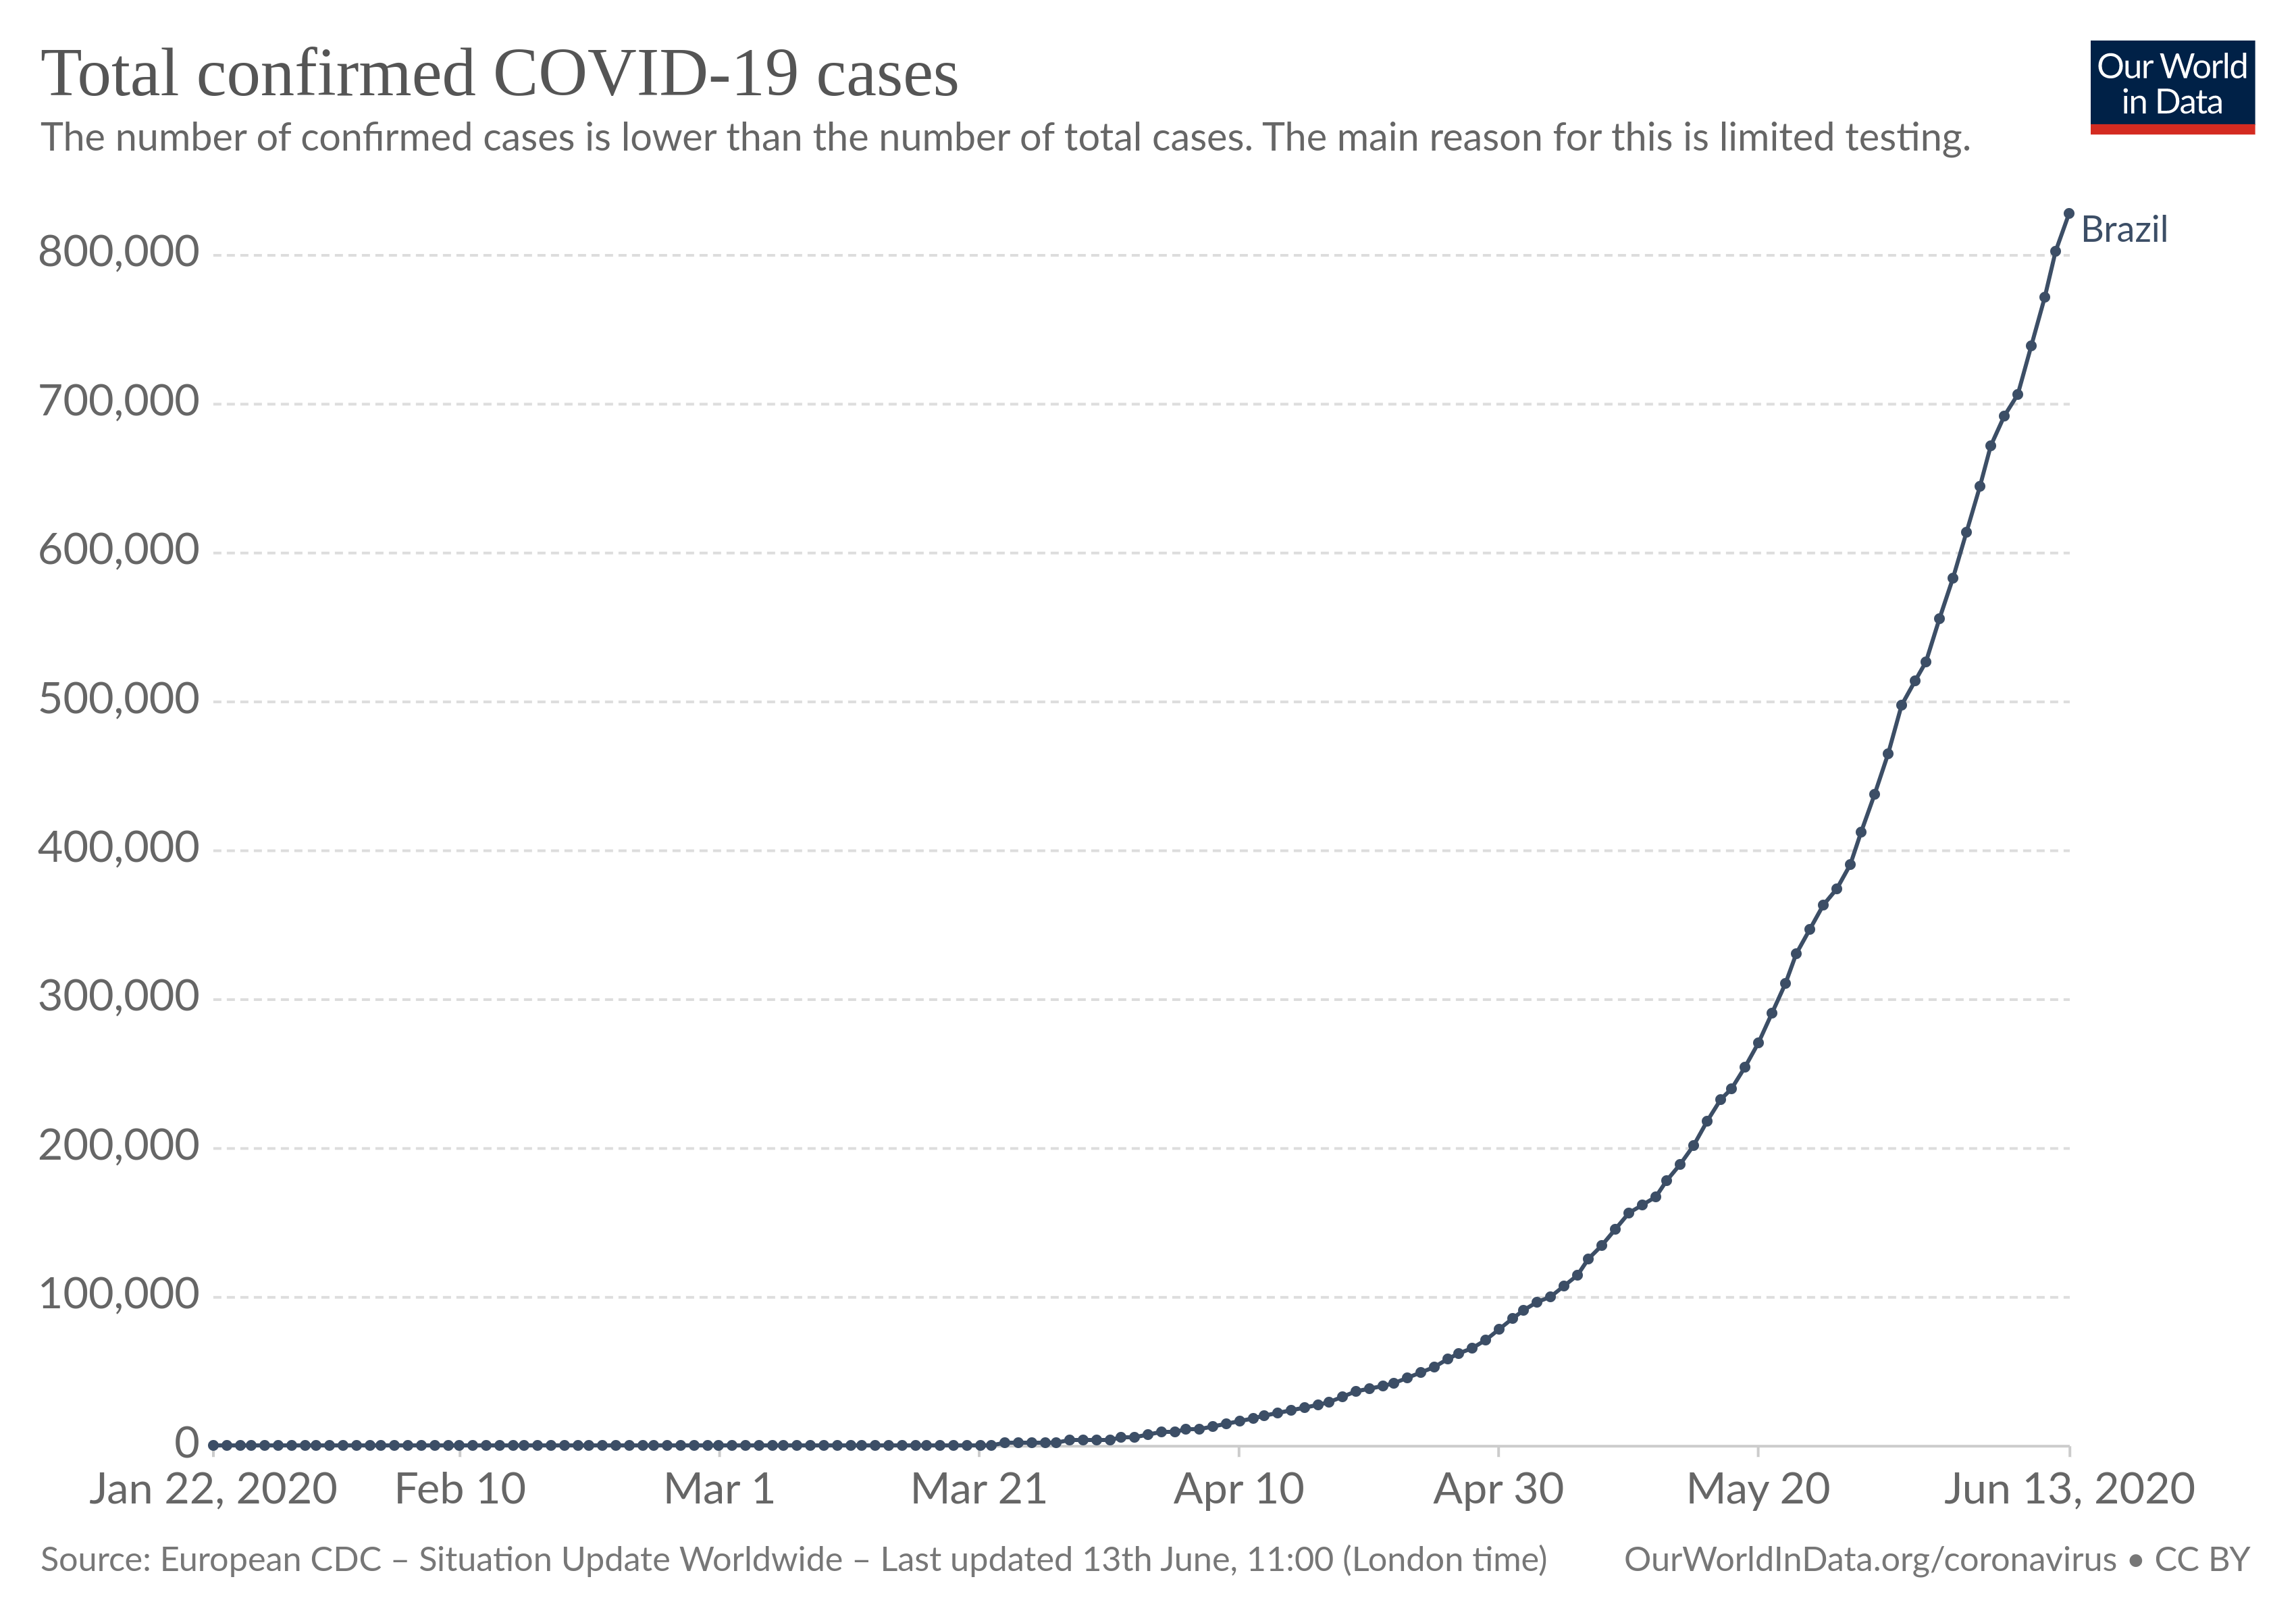
\includegraphics[width=0.7\linewidth]{Figuras/totalcasescovid19.png}

\caption{Número total de casos confirmados \\ Fonte: \textit{Our World in Data} (\url{ourworldindata.org})}
\end{figure}

O crescimento exponencial pode ser modelado pela equação:
$$
I(t) = a\times (1+b)^t,
$$
onde a constante $a$ representa a quantidade de doentes no momento em que se inicia o acompanhamento. A constante $b$ é a taxa de crescimento por unidade de tempo e depende de vários fatores.

Aplicar o logaritmo nos dois lados de uma equação nos permite resolver diversos problemas envolvendo equações exponenciais, transformando-as em equações lineares graças à propriedade do logaritmo da potência. Contudo, podemos escolher a base do logaritmo, o que nos leva ao mesmo resultado de maneiras distintas. Vamos observar isso no exemplo a seguir.

\begin{example}{Uma doença infecciosa}
Vamos supor que um grupo de $10$ pessoas tenha chegado à cidade de São Paulo portando uma nova doença extremamente infecciosa. Suponha que a taxa de crescimento da doença é de $50\%$ ao dia sem que nenhuma medida contenção seja aplicada. Vamos calcular quantos dias levará para que a doença ultrapasse $2000$ pessoas utilizando logaritmos em bases distintas:

Calculando com base $10$:
\begin{align*} &10 \times 1{,}5^t = 2000\\
\Longrightarrow& t\log 1{,}5 = \log 200\\
\Longrightarrow& t = \frac{\log 200}{\log 1{,}5} = \frac{2{,}301029995664}{0{,}17609125905568} \approx 13{,}0672584658868,
\end{align*}
onde utilizamos como aproximação os valores apresentados por uma calculadora científica.

Calculando com base $1,5$:
\begin{align*} &10 \times 1{,}5^t = 2000\\
\Longrightarrow& t\log_{1{,}5} 1{,}5 = \log_{1{,}5} 200\\
\Longrightarrow& t = \log_{1{,}5} 200 \approx 13{,}067258465887,
\end{align*}
onde utilizamos como aproximação os valores apresentados pela calculadora.

Assim apenas no $14^o$ dia, mais de $2000$ pessoas estariam doentes. 

As duas maneiras de resolver estão corretas e a calculadora mostrou o mesmo resultado para $t$ (o último algarismo está diferente, por que estamos trabalhando com aproximações e não com os números exatos). Não poderia ser diferente, pois estamos encontrando o mesmo $t$. Isso nos indica que
$$
\log_{1{,}5} 200 = \frac{\log 200}{\log 1{,}5}.
$$
\end{example}



\begin{task}{Resolvendo com bases distintas}
Vamos supor que um grupo de $10$ pessoas tenha chegado à cidade de São Paulo portando uma nova variedade de uma doença extremamente infecciosa. Suponha que a taxa de crescimento da doença é de $100\%$ ao dia sem que nenhuma medida contenção seja aplicada. Vamos calcular quantos dias levará para que a doença ultrapasse $2000$ pessoas utilizando logaritmos em base $10$ e em base $2$. Utilize as aproximações $\log 2 = 0{,}3$ e $\log_2 10 = 3{,}33$.
\end{task}


\begin{reflection}
Com base no exemplo e na atividade acima, você conseguiria imaginar (fazer uma hipótese) algum modo de calcular $\log_2 200$ utilizando apenas logaritmos em base $10$?
\end{reflection}


Os cálculos realizados nas atividades acima indicam uma propriedade que é valida em um contexto mais geral: a mudança de base (para logaritmos).

\arrange{Mudança de base}\label{secao_mud_base}


\begin{description}
\item[Teorema]\label{teo_mud_base}
[da mudança de base] Dados números reais positivos $a,b$ e $c$, com $a \neq 1$, temos que
$$
\log_c b = \frac{\log_a b}{\log_a c}.
$$
\end{description}
\begin{proof}
O logaritmo de $b$ em base $c$ é, por definição, o expoente ao qual devemos elevar $c$ para obter $b$. Assim, basta mostrarmos que $c^{\log_a b/\log_a c} =b$, o que pode calculado lembrando que $a^{\log_a c}=c$:
\begin{align*}
c^{\log_a b/\log_a c} = (a^{\log_a c})^{\log_a b/\log_a c} =a^{\log_a c\log_a b/\log_a c} =  a^{\log_a b} = b,
\end{align*}
onde utilizamos a propriedade da exponencial que $(a^x)^{y/x} = a^{xy/x}$.
\end{proof}



\begin{task}{Logaritmos com mudança de base}
Determine o valor dos logaritmos abaixo, sabendo que $\log 2 = 0{,}301$, $\log 3 = 0{,}477$ e $\log 7 = 0{,}845$:
\begin{enumerate}
\item $\log_3 7$;
\item $\log_7 21$;
\item $\log_9 16$.
\end{enumerate}
\end{task}


\begin{observation}{Com a calculadora}
A propriedade da mudança de base é fundamental para calcularmos logaritmos efetivamente, pois a grande maioria das calculadoras e softwares \textbf{não calcula logaritmos em qualquer base}, mas somente em base $10$ ou base $e$ (que estudaremos posteriormente). Assim, para calcular logaritmos de outras bases com a calculadora, precisamos utilizar o teorema da mudança de base, por exemplo:
$$
\log_3 25 = \frac{\log 25}{\log 3} \approx \frac{1{,}397940008672}{0{,}4771212547197} \approx 2{,}9299470414356
$$
\end{observation}


\begin{task}{Com a calculadora}
Utilize uma calculadora ou aplicativo de celular para calcular:
\begin{enumerate}
\item $\log_2 375$;
\item $\log_7 698$;
\item $\log_{2{,}71} 166$.
\end{enumerate}
\end{task}


\exercise


Assim o proprietário ficou com o veículo por dois anos.

\begin{enumerate}

\item {}\label{fuvest}

\textbf{(Fuvest)} Se $x = \log_4 7$ e $y = \log_{16} 49$, então $x - y$ é igual a:

\item {}\label{calculemudbase}

Utilizando as aproximações $\log_{10} 2 =0{,}301$  e $\log_{10} 3=0{,}477$, calcule o valor de $\log_9 128$.

\item {}\label{montanteaplicado}

Um montante de R$\$ 3.359{,}79$ foi obtido de uma aplicação de R$\$ 2.500{,}00$, que foi aplicada por um determinado número (inteiro) de meses, a uma taxa de juros compostos de $3\%$ ao mês. Não foram efetuados outros depósitos no período. Escreva, usando logaritmos, uma formula que permite calcular o tempo em que esse capital ficou aplicado, em seguida, calcule esse tempo utilizando uma calculadora.

\item {}\label{veiculodeprec}

Um veículo que foi adquirido por R$\$ 40.000{,}00$ sofre taxa de depreciação de $20\%$ ao ano. Depois de um determinado tempo o dono quis vender o carro e verificou que depois desse tempo o veículo tinha um valor de R$\$25.600,00$. Escreva, usando logaritmos, a fórmula que permite calcular depois de quanto tempo o carro estava sendo vendido, em seguida, calcule esse tempo.
\end{enumerate}

\explore{Função logarítmica}



A audição é o sentido que nos faz perceber ondas de pressão no ar, chamadas de ondas acústicas. A intensidade sonora dessas ondas mede quanta energia a onda é capaz de transmitir e a unidade frequentemente utilizada é o \textit{watt por metro quadrado} $W/m^2$. Quanto maior a potência, mais alto percebemos o som; mas a nossa percepção do aumento do som depende do som já presente no ambiente. Por exemplo uma pessoa falando em uma sala quieta pode parecer bastante alto, enquanto a mesma pessoa falando em um show de rock não faz diferença alguma.


Para lidarmos com o modo como percebemos o som e a potência das ondas sonoras, utilizamos uma unidade chamada de \textbf{decibel (dB)} que mede o \textit{nível sonoro} dos sons em relação a o limiar da audição humana. Observe a Tabela \ref{tab_decibeis} com diferentes sons, seus níveis sonoros em decibéis, suas intensidades sonoras em $W/m^2$ e percepções ao ouvido humano

\begin{table}[H]
\centering

\begin{tabu} to \textwidth{|l|c|l|l|}
\hline
\thead
Fonte do som & \makecell{Nível \\ (dB)} & \makecell{Intensidade \\($\bm{W/m^2}$)} & Percepção\\
\hline
Arma de fogo próxima ao ouvido & $130$ & $10$ & Dor\\
\hline
Avião decolando & $120$ & $1$ & Desconforto\\
\hline
Perfuratriz pneumática & $110$ & $10^{-1}$ & Muito alto\\
\hline
Sirene & $100$ & $10^{-2}$ & \\
\hline
Buzina alta & $90$ & $10^{-3}$ & Alto\\
\hline
Porta batendo & $80$ & $10^{-4}$ & \\
\hline
Rua com tráfego pesado & $70$ & $10^{-5}$ & Barulhento\\
\hline
Conversa animada & $60$ & $10^{-6}$ & \\
\hline
Conversa normal & $50$ & $10^{-6}$ & Moderado\\
\hline
Rádio volume baixo & $40$ & $10^{-8}$ & Quieto\\
\hline
Noite tranquila no campo & $30$ & $10^{-9}$ & \\
\hline
Sala quieta & $20$ & $10^{-10}$ & Muito quieto\\
\hline
Sussurrar da folhas & $10$ & $10^{-11}$ & \\
\hline
Limiar da audição & $0$ & $10^{-12}$ & \\
\hline
\end{tabu}

\captionsetup{justification=Centering}
\caption{Níveis sonoros e intensidades sonoras \\ Fonte: Adaptado de um artigo de \url{EEWeb.com} por Andrew Carter} \label{tab_decibeis}
\end{table}


\begin{reflection}
A percepção da altura de um som é subjetiva e depende da distância da fonte emissora, que não está escrita na tabela. Levando isso em consideração, você concorda com as percepções da coluna da direita?\\
Notamos que o nível sonoro (em dB) aumenta de 10 em 10 para os valores tabelados. E a intensidade sonora, como ela varia entre os diferentes níveis? 
\end{reflection}

A intensidade sonora é multiplicada por $10$ quando soma-se $10$ ao nível sonoro. Isso quer dizer que o decibel mede quantas ordens de magnitude a intensidade do som está em relação ao limiar da audição humana e multiplica o número de ordens de magnitude por $10$. Isso apreende o fato de ser necessária uma mudança drástica na intensidade para \textit{percebermos}  uma mudança no nível do som. Por exemplo uma pessoa falando à altura de $50db$ em um show de rock à altura $110db$ não muda a percepção de barulho.

\begin{observation}{O decibel (dB)}
O \textbf{decibel (dB)} é uma unidade logarítmica utilizada para medir o nível sonoro. Toma-se como referência o menor som audível ao ouvido humano $I_0$ (que é considerado com intensidade sonora de $10^{-12}\, watts/m^2$) e o decibel indica quantas ordens de grandeza uma onda sonora tem em relação à onda de referência através da expressão:
$$
I_{dB} = 10 \log_{10} \left(\frac{I}{I_0}\right),
$$
onde $I$ é a intensidade acústica, medida em watts por metro quadrado. Utilizando a propriedade do logaritmo do quociente vemos que o nível sonoro pode ser calculado, equivalentemente, por
$$
I_{dB} = 120 + 10 \log_{10} I.
$$
\end{observation}


\begin{task}{Fogos de Artifício}
Algumas cidades brasileiras estão limitando o nível sonoro dos fogos de artifício utilizados em celebrações, permitindo apenas fogos de até $100dB$ a 100 metros de distância. A classificação do som como forte ou fraco está relacionada à intensidade sonora, medida em watts por metro quadrado $W/m^2$. A menor intensidade sonora audível ou limiar de audibilidade possui intensidade $I_0 = 10^{-12} W/m^2$. O nível sonoro pode ser calculado a partir da intensidade da onda pela expressão $I_{dB} = 10 \times log(I/I_0)$, onde $I_0$ é o limiar de audibilidade. Um técnico mede a intensidade sonora de um foguete como sendo de $3{,}7 W/m^2$ a 100 metros de distância. Esse foguete poderia ser utilizado de acordo com a norma determinada por essas cidades?
\end{task}


\arrange{Função logarítmica}

Os sons na natureza podem ter os mais diversos valores, e não estarem definidos apenas para intensidades $I = 10^n$, para algum valor $n \in \mathbb{Z}$, como na Tabela \ref{tab_decibeis}. Assim o nível sonoro, em decibéis, é uma \textit{função} da intensidade sonora ($I$) do som:
$$
I_{dB}(I) = 10 \log_{10} \left(\frac{I}{10^{-12}}\right).
$$

Esse é um exemplo de uma função logarítmica!

\begin{description}
\item[Definição]\label{teo_mud_base}
Dado um número real positivo $a$, $a \neq 1$, chama-se \textbf{função logarítmica de base} $a$ à função $f: \mathbb{R}_+^* \to \mathbb{R}$ definida pela lei
$$
f(x) = \log_a x.
$$
\end{description}

\begin{observation}{A função calcula o logaritmo dos números reais positivos}
Ou seja, a função logarítmica de base $a$ é aquela que associa a cada número real positivo o logaritmo daquele número.
\end{observation}


\begin{task}{Gráficos dos logaritmos}
Utilize as aproximações abaixo, com dois dígitos de precisão, dos logaritmos em base $2$ para esboçar o gráfico de $f(x) = \log_{2} x$ no espaço quadriculado abaixo.
\begin{align*}
& \log_{2} 1/8 = -3; \,\, \log_{2} 1/4 = -2; \,\, \log_{2} 1/2 = -1; \,\, \log_{2} 1 = 0; \,\, \log_{2} 2  = 1; \,\, \log_{2} 3  =  1{,}58; \,\,\\
& \log_{2} 4  = 2; \,\, \log_{2} 5 = 2{,}32; \,\, \log_{10} 1 = 0; \,\, \log_{2} 6 = 2{,}58; \,\, \log_{2} 7  = 2{,}8; \,\, \log_{2} 8  = 3; \,\,\\
& \log_{2} 9  = 3{,}16; \,\, \log_{2} 10  = 3{,}32.
\end{align*}
Após esboçar esse gráfico, converse com seus colegas e com o professor como utilizar esses valores para esboçar o gráfico $g(x) = \log_{1/2} x$ e tente traçá-lo.
\end{task}


\begin{figure}[H]
\centering

\resizebox{\linewidth}{!}{
\begin{tikzpicture}
\foreach \i in {0,...,100}{% 10 (instead of 9) is used here to make sure the last line is drawn.
            \draw[lightgray] (0.1*\i,0) -- (0.1*\i,10);
            \draw[lightgray] (0,0.1*\i) -- (10,0.1*\i);}
\foreach \n in {0,...,10}{% 10 (instead of 9) is used here to make sure the last line is drawn.
            \draw[gray] (\n,0) -- (\n,10);
            \draw[gray] (0,\n) -- (10,\n);
            \node at (\n-0.2, 3.7) {\n};}
\foreach \n in {-4,...,6}{\node at (-0.2, \n+3.7) {\n};}
\draw[black,->] (0,-0.3) -- (0,10.3);
\node[black] at (-0.2,10.3) {y};
\draw[black,->] (-0.3,4.0) -- (10.3,4.0);
\node[black] at (10.3,3.7) {x};
\end{tikzpicture}}
\end{figure}

\begin{observation}{Invertendo a base}
A atividade \textit{Gráficos dos logaritmos} pode ser realizada se percebermos que $\log_{1/2} x = -\log_{2} x$. Essa propriedade é uma consequência do teorema da mudança de base:
$$
\log_{1/a} x = \frac{\log_a x}{\log_a {1/a}} = \frac{\log_a x}{-1} = -\log_a x. 
$$
\end{observation}


\begin{reflection}{O domínio contém apenas o semieixo positivo!}
Por que calculamos apenas os logaritmos de números reais positivos? Qual seria o problema para calcular $\log_2 (-4)$?
\end{reflection}


\begin{task}{Comparando funções conhecidas}
As curvas na figura representam as funções $f(x) = 2x-3$, $g(x)=2x^2-1$, $h(x)=1{,}5^x$ e $l(x)=\log_2 x$. Identifique que curva representa cada função. Calcular o valor da função para alguns valores de $x$ pode auxiliar na identificação.

\begin{figure}[H]
\centering

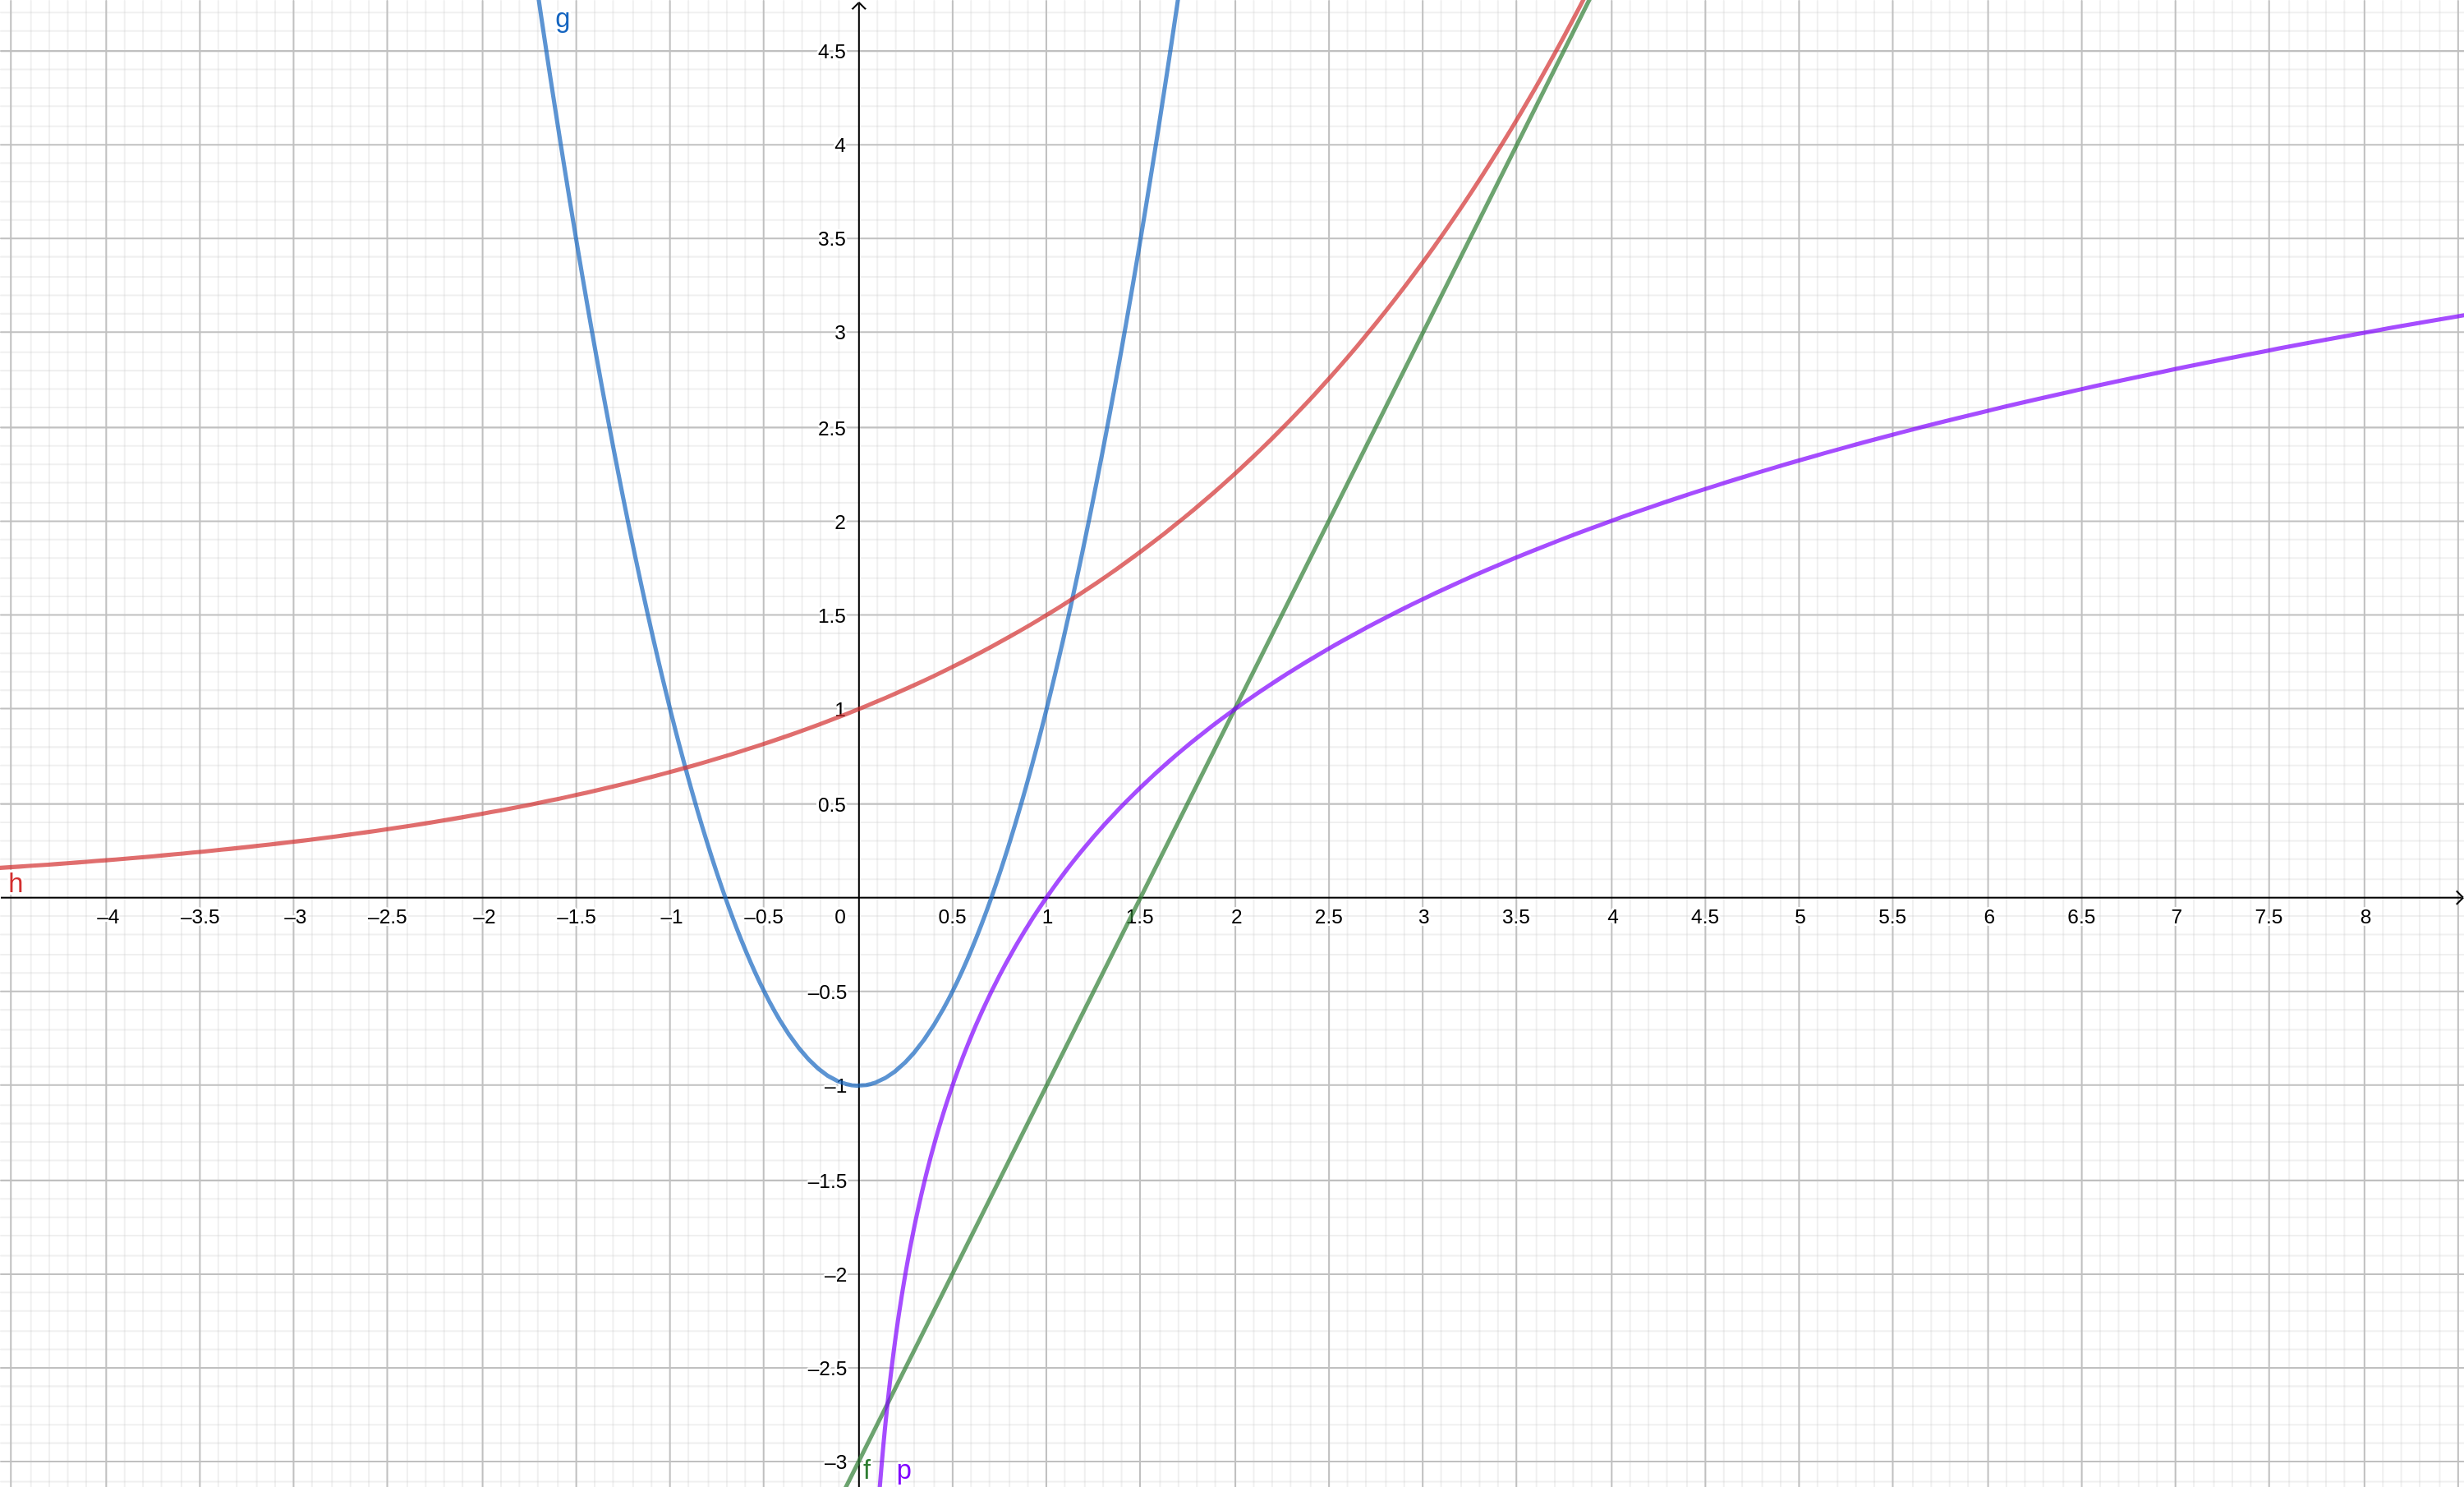
\includegraphics[width=0.8\linewidth]{Figuras/graficos_varias_funcoes}
\end{figure}

\end{task}


\begin{example}{Crescimento logarítmico e exponencial}
A figura abaixo mostra o total de mortes confirmadas causadas pela Covid-19 na França a cada dia, entre 15 de fevereiro e 13 de junho. Observamos no gráfico uma mudança no padrão da curva por volta da data de 7 de abril. No período inicial a curva é melhor aproximada por uma exponencial e depois é melhor aproximada por uma função logarítmica.

\begin{figure}[H]
\centering

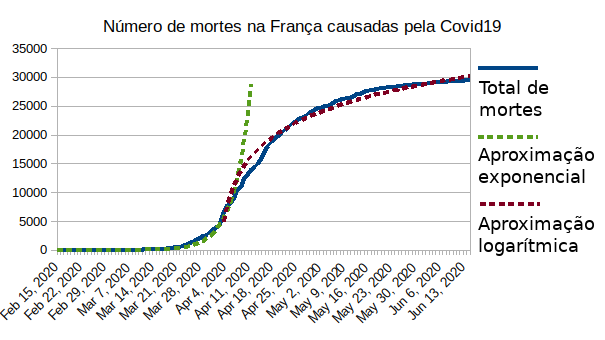
\includegraphics[width=0.95\linewidth]{Figuras/mortes_franca}
\caption{Fonte: Dados do site \textit{Our World in Data} (\url{ourworldindata.org})}
\end{figure}


Buscar uma função que melhor aproxime os dados de um determinado experimento ou acontecimento da vida real é um procedimento, chamado \textit{ajuste de curvas}, muito utilizado em todas as áreas da ciência. Os ajustes de curvas podem ser utilizados para prever tendências em dados futuros e permitir que sejam tomadas medidas preventivas.

A curva exponencial sugere que haveria um crescimento muito rápido no número de mortes. Contudo a redução posterior mostra um número muito menor, que pode ter sido causada pelas medidas adotadas pelo governo Francês (entre outras possibilidades).
\end{example}



\begin{task}{Brasil e Reino Unido na Pandemia}
Observando o gráfico abaixo, em que data (aproximadamente) o crescimento mudou de exponencial para logarítmico no Reino Unido? E no Brasil? Apesar do número ser parecido na data final do gráfico, você acredita que o número total de mortos manteve-se próximo? Que fatores sociais, econômicos e demográficos podem ter influenciado o desenvolvimento da pandemia nesses países? 

\begin{figure}[H]
\centering
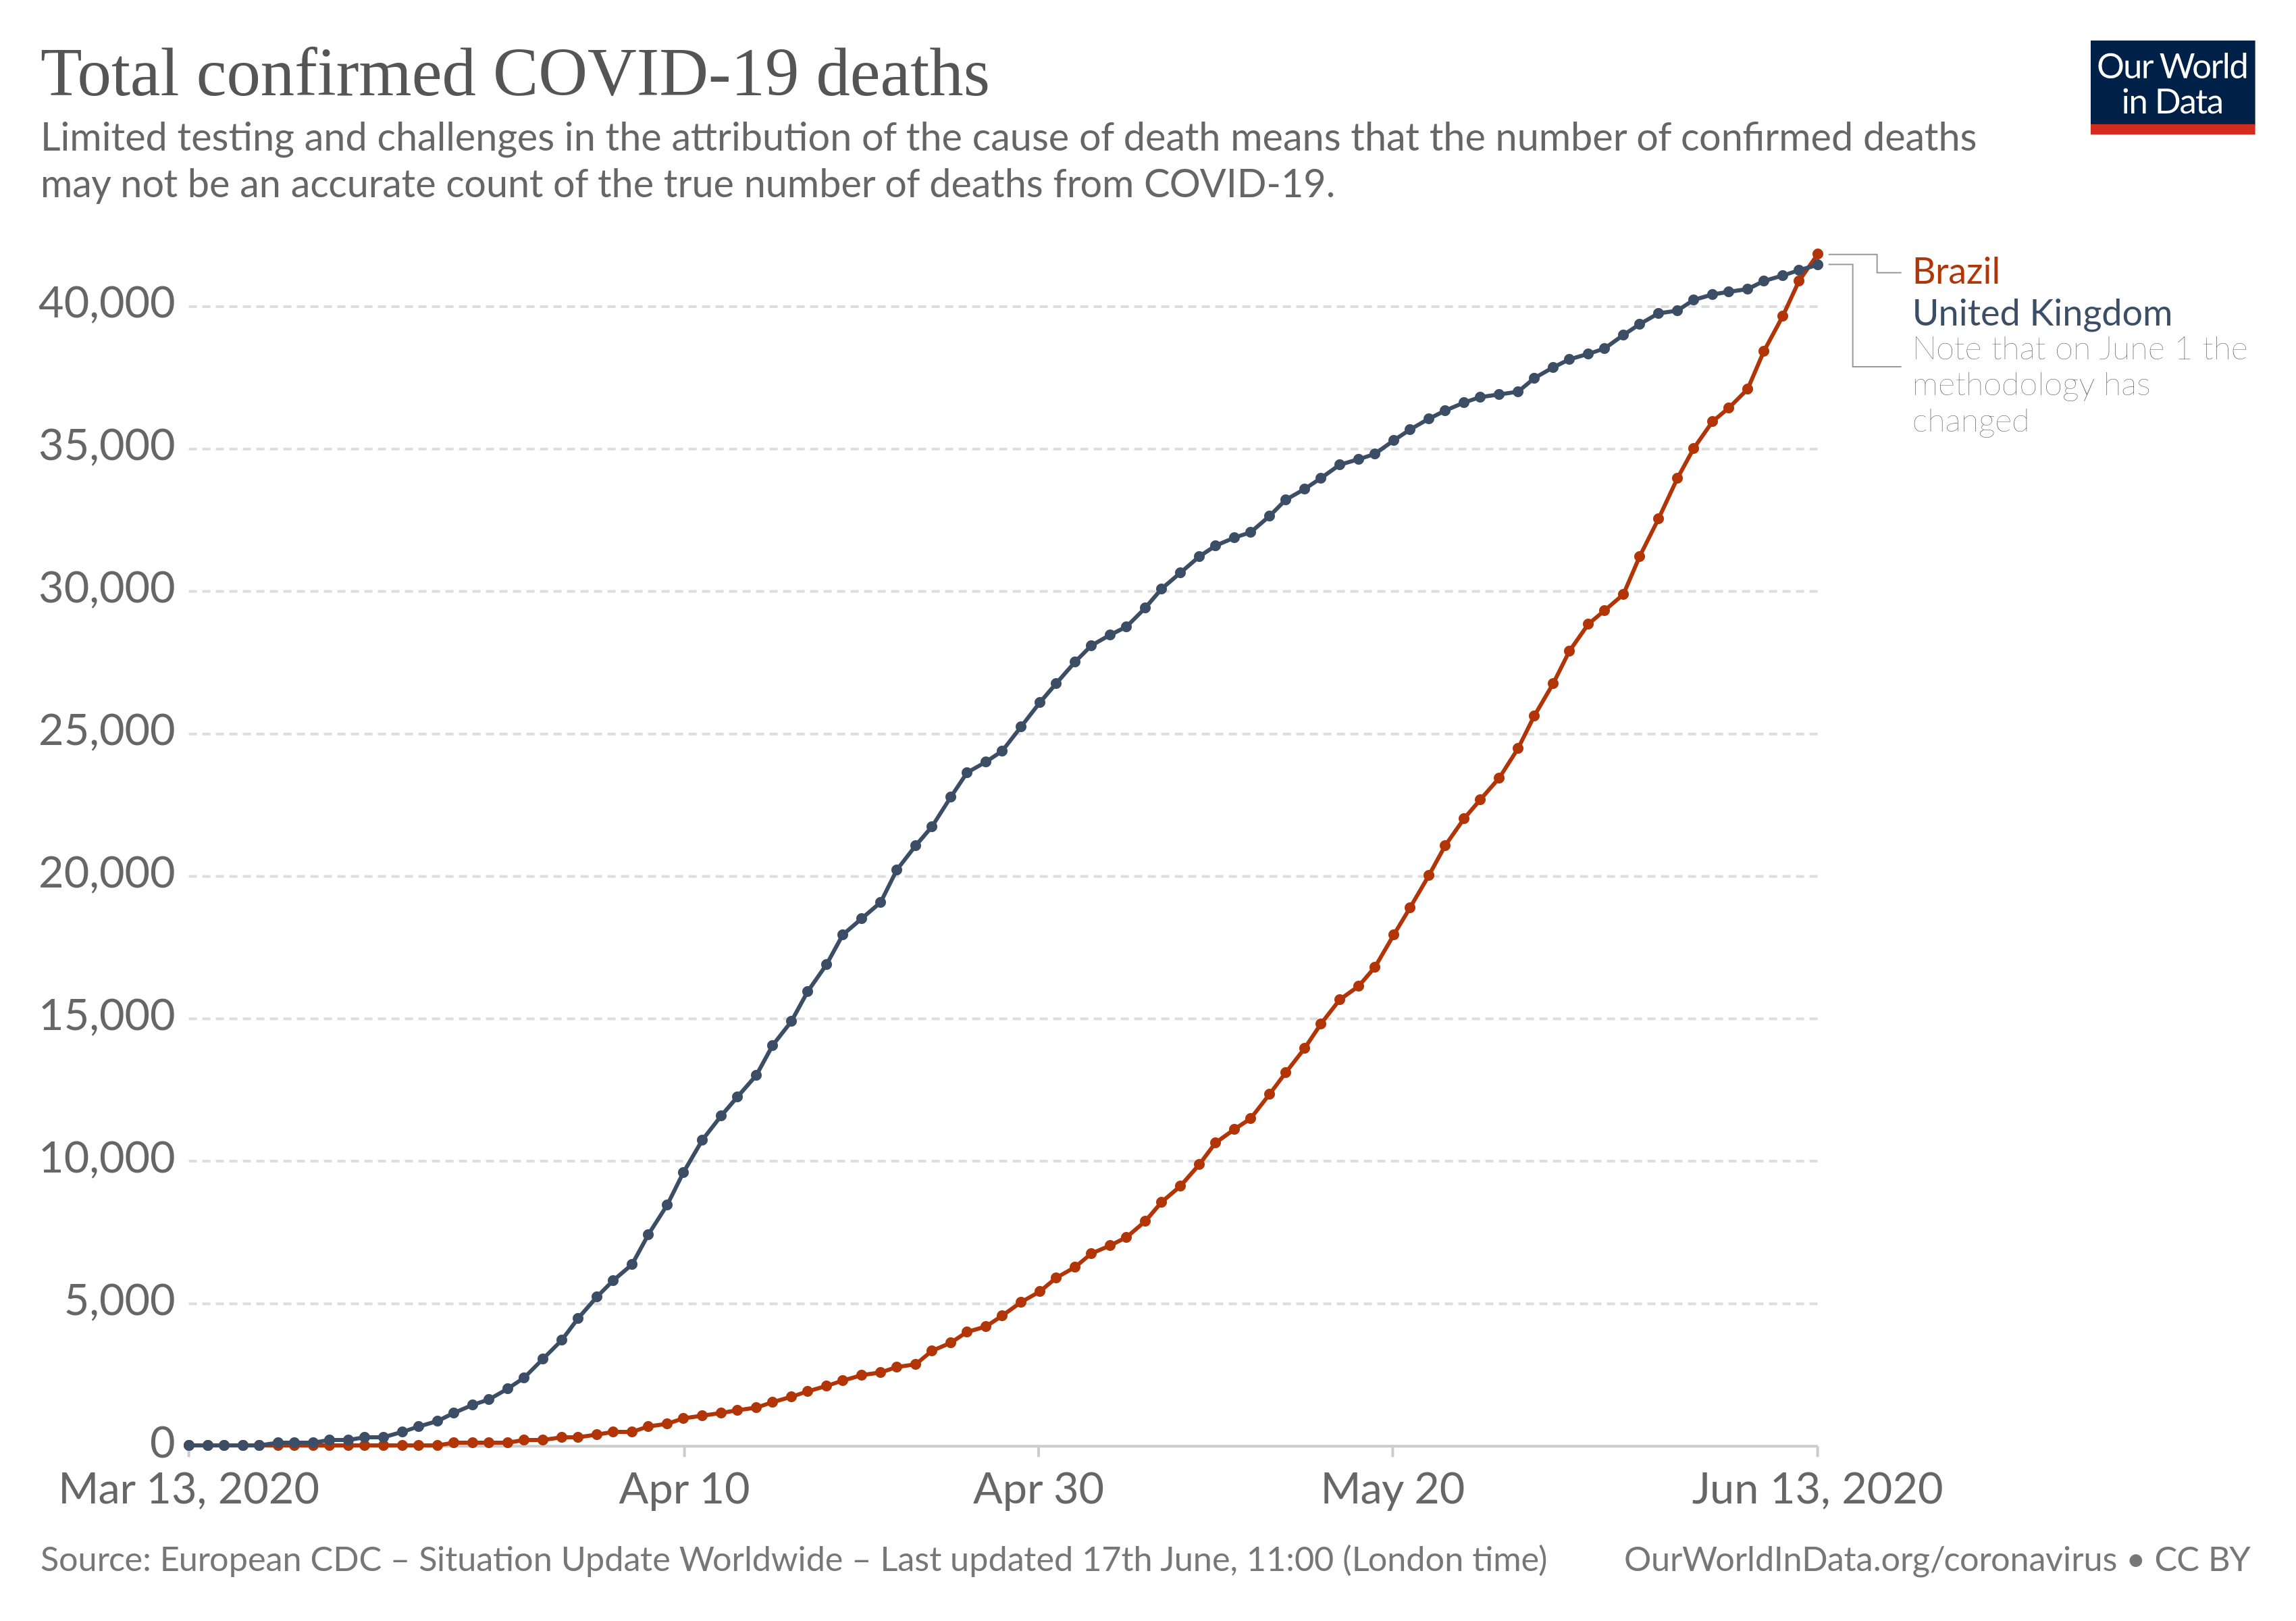
\includegraphics[width=0.8\linewidth]{Figuras/Brasil_Inglaterra_mortes.png}

\caption{Mortes confirmadas Covid-19 no Brasil e no Reino Unido. \\ Fonte: \textit{Our World in Data} (\url{ourworldindata.org}}
\end{figure}
\end{task}


\explore{Funções logarítmicas e exponenciais}



O gráfico abaixo ilustra as funções $f(x)=2^x$ (verde), $g(x)=\log_2 x$ (azul) e a função $h(x)=x$

\begin{figure}[H]
\centering

\includegraphics[width=0.8\linewidth]{Figuras/Fun_Exp_Log.png}
\caption{Funções exponencial e logarítmica de mesma base.}

\end{figure}

Para qualquer base $a>0$, $a \neq 1$, temos que $f(x)=a^x$ e $g(x)=\log_a x$ são simétricas em relação à função $h(x)=x$. Podemos utilizar um computador ou celular para acessar a atividade do GeoGebra abaixo e verificar, utilizando o controle deslizante, que essa simetria verifica-se para as mais diversas bases.

\begin{figure}[H]
\centering

\includegraphics[width=.3\linewidth]{Figuras/QRcode_exp_log.png}

\url{https://www.geogebra.org/calculator/wx7fkdk7}
\end{figure}


\begin{research}
Utilize o applet do geogebra para investigar o que ocorre com os gráficos de $f(x)=a^x$ e $g(x)=\log_a x$ quando $a=1$. Por que você acha que isso ocorre?
\end{research}


\begin{observation}{O logaritmo e a exponencial são inversas}
Se um ponto $(x,y)$ está no gráfico da função exponencial de base $a$, então $y= a^x$. Agora, se calcularmos $\log_a y$ obtemos $x$ (pois $x$ é o expoente ao qual devemos elevar $a$ para obter $y$), de modo que o ponto $(y,x)$ está no gráfico da função logarítmica de base $a$. Essa simetria traduz, então, o fato das funções logarítmicas e exponenciais serem inversas: dada uma base real $a>0$, $a \neq 1$, e números reais $x>0$ e $y$ qualquer, temos
\begin{align*}
& a^{\log_a x}=x,\\
& \log_a (a^y) = y.
\end{align*}
\end{observation}


\begin{task}{Funções inversas na prática}
Complete a tabela abaixo calculando a exponencial do logaritmo e o logaritmo da exponencial.

\begin{table}[H]
\centering

\begin{tabu} to \textwidth{|c|c|c|}
\hline
\thead
$\bm{x}$ & $\bm{y=2^x}$ & $\bm{{\log_2 x}}$ \\
\hline
$1$ & & \\
\hline
$2$ & & \\
\hline
$3$ & & \\
\hline
$4$ & & \\
\hline
\end{tabu}
\hspace{2em}
\begin{tabu} to \textwidth{|c|c|c|}
\hline
\thead
$\bm{y}$ & $\bm{x=3^y}$ & $\bm{{\log_3 x}}$ \tabularnewline
\hline
$-1$ & & \\
\hline
$1$ & & \\
\hline
$0$ & & \\
\hline
$2$ & & \\
\hline
\end{tabu}

\end{table}
\end{task}


\begin{reflection}
Você consegue explicar por que $a^{\log_a x}=x$ e $\log_a (a^y) = y$? Tente discutir com seus colegas por que essas igualdades valem.
\end{reflection}


Uma consequência do fato de que as funções logarítmicas e exponenciais são inversas, é que funções logarítmicas de bases distintas são muito parecidas. É possível multiplicar uma delas por uma constante para obter a outra.


\begin{task}{Funções logarítmicas distintas}
No \textit{applet} do GeoGebra, disponível através do atalho abaixo, podemos mover a barra com o valor $a$, alterando o gráfico da função $h(x) = a \log_2 x$. Qual o valor de $a$ para que o gráfico de $h(x)$ coincida com o gráfico de $f(x) = \log_{1{,}2} x$?


\begin{figure}[H]
\centering


\includegraphics[width=.3\linewidth]{Figuras/QRcode_mult_constante.png}

\url{https://www.geogebra.org/calculator/qyuzhbmp}
\end{figure}

\textbf{Desafio:} aplique o Teorema da mudança de base em $g(x)= \log_2 x$, utilizando a base $1{,}2$ para encontrar algebricamente o valor de $a$.
\end{task}


\begin{observation}{Funções logarítmicas de bases distintas}
Podemos utilizar o fato das funções exponenciais e logarítmicas serem inversas para trocar as bases de funções logarítmicas:
\begin{align*}
&\log_a x = \log_a b^{\log_b x} =\log_a b\log_b x.
\end{align*}
Ou seja a função $\log_a x$ é igual à função $\log_b x$ multiplicada pela constante $\log_a b$. Essa constante pode ser negativa se $a<b$.
\end{observation}

A figura abaixo ilustra os gráficos de funções logarítmicas de bases distintas (base maior do que 1 na cor laranja e menor do que 1 na cor verde).

\begin{figure}[!htb]
\centering
\includegraphics[width=0.8\linewidth]{Figuras/Graficos_logs.png}
\caption{Funções logarítmicas de bases distintas.}
\end{figure}


\begin{observation}{Funções logarítmicas crescentes e decrescentes}
Observamos na figura, imediatamente, que as funções logarítmicas de base maior do que 1 são crescentes. Isso ocorre porque as exponenciais de base $a>1$ são funções estritamente crescentes:
$$
x > y \Longleftrightarrow a^x > a^y,
$$
ou seja, para $x=\log_a c$ e $y=\log_a d$, temos
$$
\log_a c > \log_a d \Longleftrightarrow c > d.
$$
Também observamos que as funções logarítmicas de base menor do que 1 são decrescentes. Isso ocorre porque as exponenciais de base $b<1$ são funções estritamente decrescentes:
$$
x > y \Longleftrightarrow b^x < b^y,
$$
ou seja, para $x=\log_b c$ e $y=\log_b d$, temos
$$
\log_b c > \log_b d \Longleftrightarrow c < d.
$$


\end{observation}


\exercise


\begin{enumerate}
\item {} \label{EstimaGraf}

É possível verificar rapidamente, utilizando gráficos, o tempo que uma aplicação demora para dobrar, triplicar, quadruplicar, ... o valor aplicado. O gráfico abaixo, da função $f(m)=\log_{1{,}01}(m/100)$, representa o tempo, em meses, para que determinado montante seja atingido a partir de um capital de $R\$ 100{,}00$, aplicado a uma taxa mensal de $1\%$.  Observando o gráfico, estime com erro menor do que $10$ o número de meses necessário para o capital inicial:
\begin{enumerate}
\item dobrar;
\item triplicar;
\item quadruplicar.
\end{enumerate}

\begin{figure}[H]
\centering

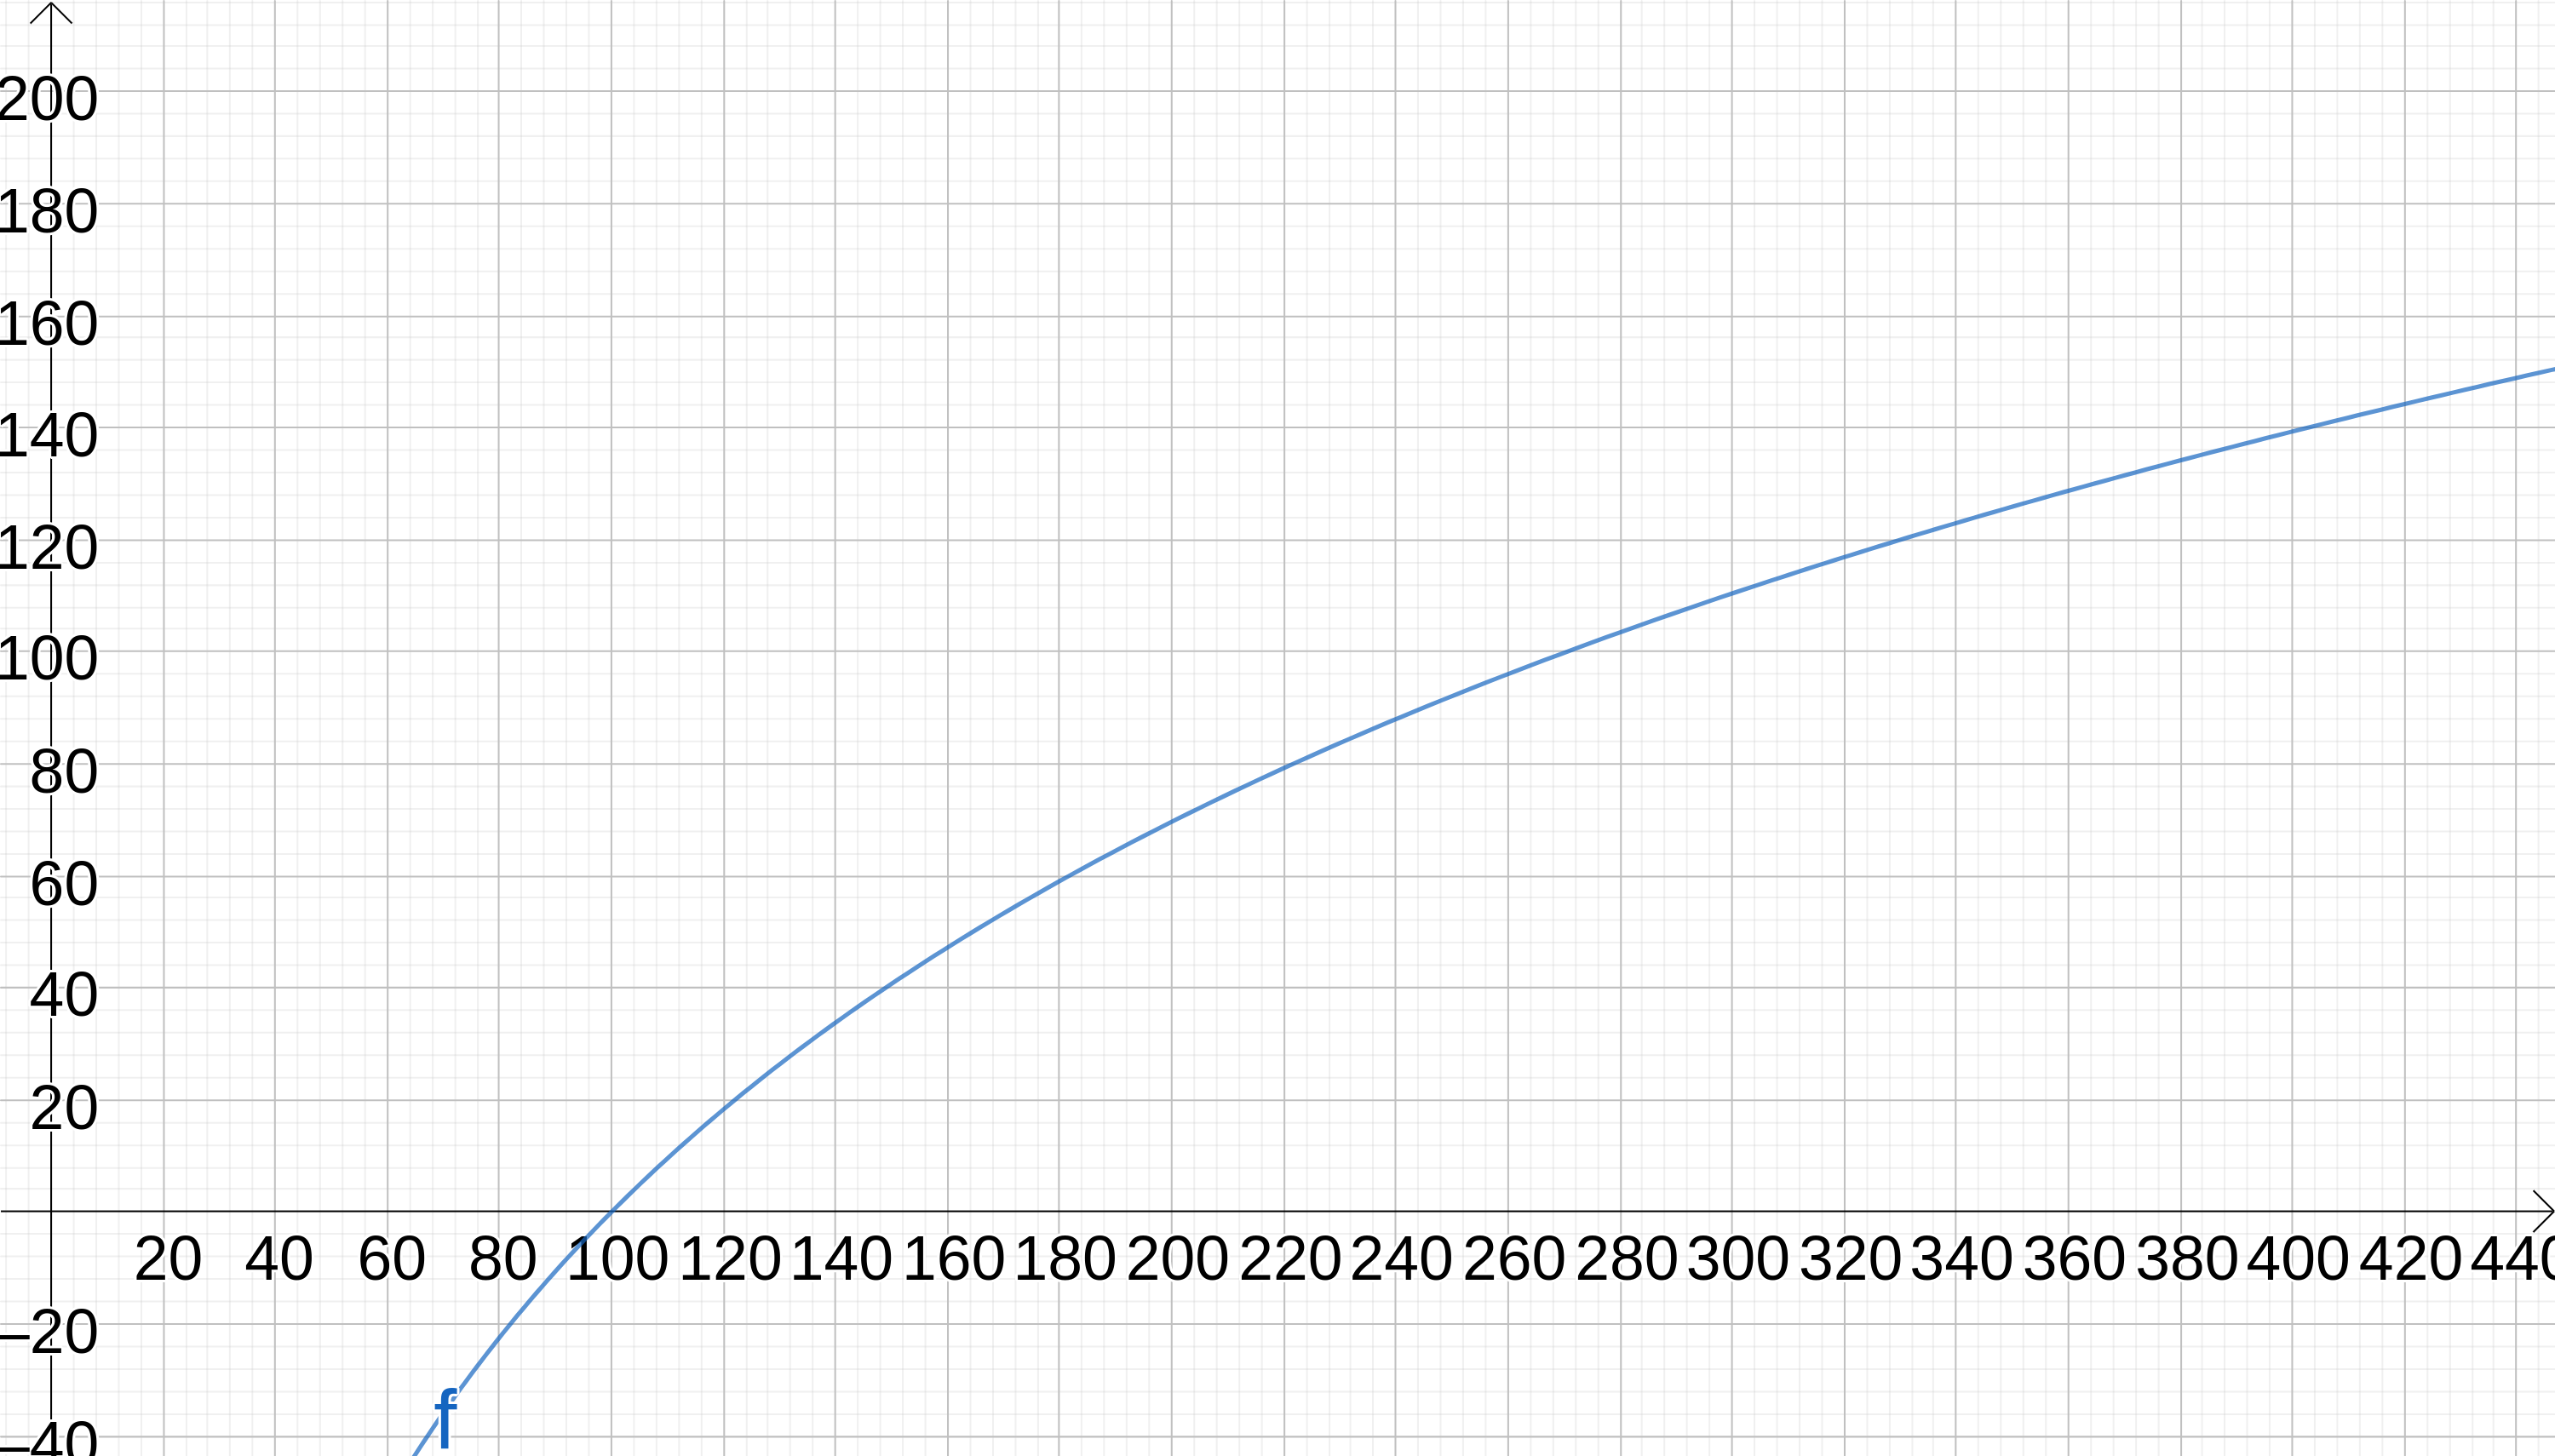
\includegraphics[width=0.8\linewidth]{Figuras/Tempo_montante.png}
\caption{Gráfico da função $f(m)=\log_{1{,}01} (m/100)$.}
\end{figure}



\item {}\label{poluicaoSonora}

\textbf{(Poluição sonora em sala de aula)} Um teste feito com um decibelímetro em uma escola, em São Carlos (SP), 
constatou que o nível de ruído emitido pelas crianças dentro de sala de aula está acima do recomendado pela Organização 
Mundial de Saúde  (OMS) e a Associação Brasileira de Normas Técnicas. A exposição a esses ruídos podem prejudicar o 
aprendizado e causar danos ao aparelho auditivo, de acordo com especialistas.
Segundo a OMS, o nível seguro de ruído em uma sala de aula não pode ultrapassar os 35 decibéis. Já para a Associação Brasileira de Normas Técnicas, o limite é de 50 decibéis.

A reportagem do Jornal da EPTV utilizou um decibelímetro para fazer a medição e o resultado em uma sala de aula chegou a 74 decibéis. O sinal da escola também ficou acima do recomendado, registrando o mesmo número. Em ambientes abertos, como o pátio, os especialistas afirmam que a tolerância é um pouco maior e os sons de até 85 decibéis não trazem riscos. “Acima de 85 decibéis e oito horas de exposição já causa lesão ao aparelho auditivo”, alerta 
o médico da Universidade de São Carlos (UFSCar), Bernardino Alves Souto.

Ainda de acordo com Souto, nível acima de 75 decibéis já se pode causar alguns sintomas. "Irritabilidade, 
insônia, 
ansiedade e dificuldade de concentração, dependendo do tempo de exposição ao barulho. Em uma sala de aula com 
aproximadamente 80 decibéis de intensidade de som, a capacidade de aprendizado e concentração da criança pode reduzir de 
20{\%} a 80{\%}”, explicou 
Souto.\footnote{Fonte:\url{
http://g1.globo.com/sp/sao-carlos-regiao/noticia/2014/01/nivel-de-ruido-em-escola-esta-acima-do-recomendado-em-sao-carlo
s-sp.html}. Acesso em: 25 set. 2017.}

 O nível sonoro (NS), medido em decibel (dB), pode ser calculado usando a fórmula $NS=10\cdot log(\frac{I}{I_0})$ onde I 
é a intensidade do som considerado e $I_0$ é a menor intensidade sonara audível, sendo  $I_0=10^{-12}$ $W/m^2$. 
Considerando 35 decibéis o nível sonoro ideal em uma sala de aula, determine a intensidade do som nesse ambiente.


\item {}\label{UFC2001}

(UFC-2001) Suponha que o nível sonoro $\beta$ e a intensidade I de um som estejam relacionados pela equação logarítmica 
$\beta = 120 + 10\cdot log_{10} I$, em que b é medido em decibéis e I, em watts por metro quadrado. Sejam $I_1$ a 
intensidade correspondente ao nível sonoro de 80 decibéis de um cruzamento de duas avenidas movimentadas e $I_2$ a 
intensidade correspondente ao nível sonoro de 60 decibéis do interior de um automóvel com ar-condicionado. A razão 
$I_1/I_2$ é igual a:
 \begin{enumerate}
     \item 1/10
     \item 1
     \item 10 
     \item 100
     \item 1 000
 \end{enumerate}


\item {}\label{Unesp2006}

(Unesp-2006) O nível sonoro N, medido em decibéis (dB) e a intensidade I de um som, medida em watt por metro quadrado 
($W/m_2$), estão relacionados pela equação $N=120+10\cdot \log_{10} (I)$. Suponha que foram medidos, em certo local, os 
níveis sonoros, $N_1$ e $N_2$, de dois ruídos com Intensidades $I_1$ e $I_2$, respectivamente. Sendo $N_1 - N_2 = 20 dB$, 
a razão $I_1/I_2$ é:
\begin{enumerate}
    \item $10^{-2}$
    \item $10^{-1}$
     \item $10$
     \item $10^{2}$
     \item $10^{3}$
\end{enumerate}


\item {} \label{Unicamp2008}

(Unicamp-2008) A escala de um aparelho para medir ruídos é definida da seguinte forma: $R = 12 + log_{10}(I)$, em que R 
é a medida do ruído, em bels, e I é a intensidade sonora, em W/m2. No Brasil, a unidade utilizada é o decibel (1/10 do 
bel). Por exemplo, o ruído dos motores de um avião a jato é de 160 decibéis, enquanto o ruído do tráfego em uma esquina 
movimentada de uma grande cidade é de 80 decibéis, sendo este o limite a partir do qual o ruído passa a ser nocivo ao 
ouvido humano. Com base nessas informações, julgue os itens que se seguem.

(1) A intensidade sonora de um ruído de zero decibel é de $10^{-12} w/m^2$. 

(2) A intensidade sonora dos motores de um avião a jato é o dobro da intensidade sonora do tráfego em uma esquina movimentada de uma grande cidade.

(3) Uma intensidade sonora maior que $10^{-4} w/m^2$ produz um ruído que é nocivo ao ouvido humano. 




\item {}\label{UCSSRS}

(UCS-RS) O nível $\beta$, em decibel, de um som que tem intensidade I é dado pela fórmula $\beta = 10 \cdot log 
(I/I_0)$, em que $I_0 = 10^{-12}$. Se a intensidade I for multiplicada por 100, em quantos decibel aumenta $\beta$?

\begin{enumerate}
    \item 2
    \item 20
    \item 100
    \item 120
    \item 140
\end{enumerate}
\end{enumerate}

\explore{Escala logarítmica}


Às vezes, em situações concretas, podemos ter magnitudes muito diferentes dentro de um conjunto de valores. Na figura abaixo, por exemplo, as circunferências têm raios proporcionais aos raios do Sol (amarelo) e dos 8 planetas do sistema solar: Mercúrio (cinza, muito pequeno para ver), Vênus (rosa), Terra (azul pálido), Marte (vermelho), Júpiter (amarelo queimado), Saturno (laranja), Urano (azul claro) e Netuno (azul).


\begin{figure}[H]
\centering


\resizebox{.7\textwidth}{!}{
\begin{tikzpicture}[background rectangle/.style={fill=black}, show background rectangle]
\draw[fill=yellow] (0,0) circle [radius=6.963];
\draw[fill=gray] (7.2,0) circle [radius=0.024];
\draw[fill=pink] (7.5,0) circle [radius=0.0605];
\draw[fill=blue!60!white] (7.8,0) circle [radius=0.0637];
\draw[fill=red] (8.1,0) circle [radius=0.034];
\draw[fill=olive!40!orange] (9,0) circle [radius=0.69911];
\draw[fill=olive!20!orange] (10.4,0) circle [radius=0.58232];
\draw[fill=blue!30!white] (11.4,0) circle [radius=0.253];
\draw[fill=blue] (12,0) circle [radius=0.246];
\draw[color=white](-7.2,1)--(-7.5,1)node[color=white,left,font=\large]{100};  
\draw[color=white](-7.2,5)--(-7.5,5)node[color=white,left,font=\large]{500};     
\draw[color=white](-7.2,0)--(-7.5,0)node[color=white,left,font=\large]{0};
\draw[color=white](-7.2,0)--(-7.2,7);
\end{tikzpicture}}

\caption{O sol e os planetas em escala linear (em milhares de quilômetros).}\label{log_planetas}
\end{figure}


É muito difícil ver os planetas menores na figura. Para lidar com dados de magnitudes muito distintas, com frequência, utiliza-se uma escala logarítmica (a mesma da régua de cálculo). Na figura abaixo observamos os mesmos objetos em uma escala logarítmica (branca).


\begin{figure}[H]
\centering

\resizebox{.7\textwidth}{!}{
\begin{tikzpicture}[background rectangle/.style={fill=black}, show background rectangle]
\draw[fill=yellow] (0,0) circle [radius=(ln(696.3)/ln(10))];
\draw[fill=gray] (3.4,0) circle [radius=(ln(2.4)/ln(10))];
\draw[fill=pink] (4.8,0) circle [radius=(ln(6.05)/ln(10))];
\draw[fill=blue!60!white] (6.6,0) circle [radius=(ln(6.38)/ln(10))];
\draw[fill=red] (8.1,0) circle [radius=(ln(3.4)/ln(10))];
\draw[fill=olive!40!orange] (10.7,0) circle [radius=(ln(69.911)/ln(10))];
\draw[fill=olive!20!orange] (14.7,0) circle [radius=(ln(58.232)/ln(10))];
\draw[fill=blue!30!white] (18,0) circle [radius=(ln(25.3)/ln(10))];
\draw[fill=blue] (21,0) circle [radius=(ln(24.6)/ln(10))];
\draw[color=white](-3,2)--(-3.2,2)node[color=white,left,font=\large]{100};  
\draw[color=white](-3,3)--(-3.2,3)node[color=white,left,font=\large]{1000};  
\draw[color=white](-3,1)--(-3.2,1)node[color=white,left,font=\large]{10};     
\draw[color=white](-3,0)--(-3.2,0)node[color=white,left,font=\large]{0};
\draw[color=white](-3,0)--(-3,3);
\draw[color=gray](-4.5,2)--(-4.7,2)node[color=gray,left,font=\large]{2};  
\draw[color=gray](-4.5,3)--(-4.7,3)node[color=gray,left,font=\large]{3};  
\draw[color=gray](-4.5,1)--(-4.7,1)node[color=gray,left,font=\large]{1};     
%\draw[color=gray](-10.2,0)--(-10.7,0)node[color=gray,left,font=\Huge]{0};
\draw[color=gray](-4.5,0)--(-4.5,3);
\end{tikzpicture}}

\caption{O sol e os planetas em escala logarítmica (em milhares de quilômetros).}
\end{figure}


Na escala logarítmica da figura, a cada unidade linear (cinza) os valores são \textit{multiplicados} por 10, de modo que os raios dos planetas têm valores correspondentes à escala logarítmica (branca).


\begin{observation}{Colocar um gráfico em escala logarítmica.}
A escala cinza na Figura \ref{log_planetas} explica o que fizemos para colocar o gráfico em escala logarítmica: calculamos os logaritmos dos raios dos planetas e fizemos novas circunferências com raios iguais a esses logaritmos. Como os valores da escala são as potências de 10 dos valores da escada linear, os logaritmos são exatamente os valores necessários para obter-se os respectivos valores originais nessa nova escala.
\end{observation}

\begin{task}{Ordens de magnitude dos planetas.}
Observado as circunferências e a escala logarítmica da Figura \ref{log_planetas}, qual é a melhor aproximação na comparação dos tamanhos de Vênus (rosa) e de Saturno (laranja).
\begin{enumerate}
\item O diâmetro de Saturno é o dobro do diâmetro de Vênus.
\item O diâmetro de Saturno é dez vezes o diâmetro de Vênus.
\item O diâmetro de Saturno é três vezes o diâmetro de Vênus.
\item O diâmetro de Saturno é cem vezes o diâmetro de Vênus.
\end{enumerate}
\end{task}


\begin{knowledge}
\textbf{Distâncias entre os planetas.}
Nas figuras acima apenas colocamos os "planetas"\, lado a lado. Não levamos em conta as distâncias entre eles. O sistema solar é muito maior do os raios  dos planetas e do próprio Sol. Para se ter uma ideia, a distância de Netuno ao Sol é de cerca de $4{,}5 \times 10^{9}Km$, enquanto o diâmetro do Sol é de $1{,}4 \times 10^6$. Ou seja, a distância de Netuno até o Sol é mais de 3000 vezes maior do que o diâmetro do Sol.
\end{knowledge}

\begin{example}{Comprimentos e massas de primatas.}
Às vezes estudamos dados que ocorrem em uma larga escala. Isso pode fazer com que dados significativamente distintos pareçam muito próximos e, assim, dificultar a análise. Para ilustrar isso trazemos gráfico de dispersão das massas e comprimentos médios (dados de Animal Diversity Web Quaardvark (animaldiversity.ummz.umich.edu/quaardvark)) de diversas espécies de primatas em escala logarítmica e linear

\begin{figure}[H]
\centering
\begin{multicols}{2}
\null\vfill
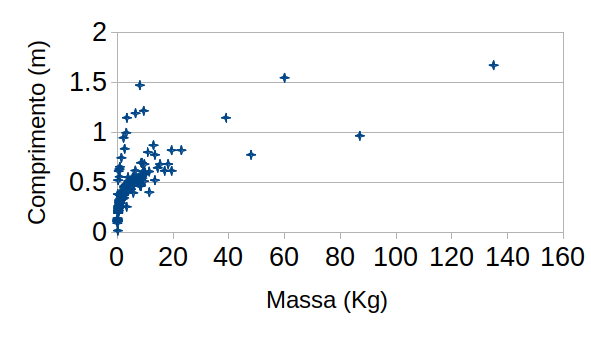
\includegraphics[width=\linewidth]{Primatas_linear.png}

Em escala linear.
\vfill\null
\columnbreak

\null\vfill
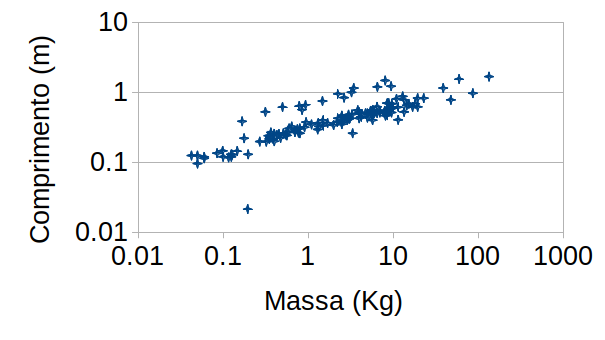
\includegraphics[width=\linewidth]{Primatas_log.png}

Em escala logarítmica.
\vfill\null
\end{multicols}
\caption{Massas e comprimentos de diversos primatas}
\end{figure}

Os dados ficam, assim, mais distribuídos e melhores para análise. Muitos dos primatas têm menos de 1 Kg e menos de 50 cm, contudo um animal  100 g e 10 cm é muito menor do que um animal de 1 Kg e 50 cm.
\end{example}

\arrange{Escala logarítmica}

Ao colocarmos um gráfico em escala logarítmica parece que "espalhamos" mais os dados de menor magnitude, que estavam condensados em uma região muito pequena. Isso ocorre pois os valores nessa escala crescem mais lentamente para valores menores do que para valores maiores. %torna iguais crescimentos relativos iguais e não as magnitudes dos dados per si.


\begin{task}{Três cidades.}
Vamos considerar as populações das cidades de Metrópolis, Smallville e Gotham City. Um censo realizado no ano 2000 verificou que elas tinham 10.000, 1.000 e 5.000 habitantes, respectivamente. Dez anos após verificou-se que elas estavam com 11.000, 2.000 e 10.000 habitantes, respectivamente. A figura da esquerda, em escala linear, apresenta as populações das cidades.


\begin{center}
\begin{minipage}[c]{0.4\linewidth}
\begin{center}
Populações em escala linear.
\begin{tikzpicture}[domain=0:5]
\draw[->] (-1,0) -- (4,0);
\draw[->] (0,-1) -- (0,5);
\draw[step=0.1,gray,thin, dotted] (0,0) grid (4,5);
\draw [fill=session1!80] (0.25,0) rectangle (0.75,4);
\draw [fill=session1!80] (2.25,0) rectangle (2.75,4.4);
\draw [fill=session2!80] (0.75,0) rectangle (1.25,0.4);
\draw [fill=session2!80] (2.75,0) rectangle (3.25,0.8);
\draw [fill=session4!80] (1.25,0) rectangle (1.75,2);
\draw [fill=session4!80] (3.25,0) rectangle (3.75,4);
\draw[dashed] (1,5) -- (1,0)node[below] {$S$};
\draw[dashed] (1.5,5) -- (1.5,0)node[below] {$G$};
\draw[dashed] (0.5,5) -- (0.5,0)node[below] {$M$};
\node at (1,-0.7) {$2000$};
\node at (3,-0.7) {$2010$};
\draw[dashed] (3,5) -- (3,0)node[below] {$S$};
\draw[dashed] (3.5,5) -- (3.5,0)node[below] {$G$};
\draw[dashed] (2.5,5) -- (2.5,0)node[below] {$M$};
\node[left] at (0,0.8) {$2000$};
\node[left] at (0,1.6) {$4000$};
\node[left] at (0,2.4) {$6.000$};
\node[left] at (0,3.2) {$8.000$};
\node[left] at (0,4) {$10.000$};
\end{tikzpicture}
\end{center}
\end{minipage}
\begin{minipage}[c]{0.4\linewidth}
\begin{center}
Populações em escala logarítmica.
\begin{tikzpicture}[domain=0:5]
\draw[->] (-1,0) -- (4,0);
\draw[->] (0,-1) -- (0,5);
\draw[step=0.1,gray,thin, dotted] (0,0) grid (4,5);
\draw[dashed] (1,5) -- (1,0)node[below] {$S$};
\draw[dashed] (1.5,5) -- (1.5,0)node[below] {$G$};
\draw[dashed] (0.5,5) -- (0.5,0)node[below] {$M$};
\node at (1,-0.7) {$2000$};
\node at (3,-0.7) {$2010$};
\draw[dashed] (3,5) -- (3,0)node[below] {$S$};
\draw[dashed] (3.5,5) -- (3.5,0)node[below] {$G$};
\draw[dashed] (2.5,5) -- (2.5,0)node[below] {$M$};
\node[left] at (0,1) {$10$};
\node[left] at (0,2) {$100$};
\node[left] at (0,3) {$1.000$};
\node[left] at (0,4) {$10.000$};
\end{tikzpicture}
\end{center}
\end{minipage}
\end{center}
No gráfico em escala logarítmica, os valores devem ser marcados na altura dos seus respectivos logaritmos. Utilizando as aproximações $\log 2 \approx 0{,}3$, $\log 5 \approx 0{,}7$ e $\log 11 \approx 1{,}04$, esboce os valores das populações na escala logarítmica à direita:
\begin{enumerate}
\item Qual cidade obteve o maior crescimento?
\item Quais cidades tiveram o maior crescimento em relação aos tamanhos de suas populações?
\end{enumerate}
\end{task}


\begin{reflection}
No gráfico de escala logarítmica, quais cidades parecem ter sofrido maior alteração em suas populações?
\end{reflection}



\begin{observation}{Crescimento relativo com logaritmos.}
Se um valor $a$ é acrescido em um percentual $p$ após um determinado período, e outro valor $b$ é acrescido também em $p$ por cento após outro período, então as diferenças entre os logaritmos dos valores (em uma base qualquer $c$, $c\neq 1$) é a mesma:
\begin{align*}
&\log_c (a(1+p))-\log_c a = \log_c ((a(1+p))/a)= \log_c (1+p)\\
&\log_c (b(1+p))-\log_c b = \log_c ((b(1+p))/b)= \log_c (1+p)
\end{align*}

Ou seja, as diferenças (distâncias no gráfico) são as mesmas. Isso significa que \textbf{em um gráfico em escala logarítmica é fácil perceber o crescimento\footnote{Estamos utilizando o termo crescimento relativo mesmo para $c<1$, o que corresponderia a um decrescimento. Todavia o conceito de Taxa de Crescimento Relativo é amplamente utilizado em diversas áreas, mesmo quando o crescimento é negativo (ou seja, há um decrescimento).} proporcional (em relação à magnitude dos valores)}.
\end{observation}



\begin{example}{Criptomoedas.}
Investidores do mercado financeiro fazem os mais variados tipos de investimentos. Uma forma que têm ganhado popularidade é a compra de criptomoedas, como o Bitcoin. Nesse investimento compram-se unidades da moeda para revenda posterior por um preço maior. O gráfico abaixo ilustra o valor da Bitcoin, dia a dia, no período indicado (dados de \url{coindesk.com}).

\begin{figure}[H]
\centering

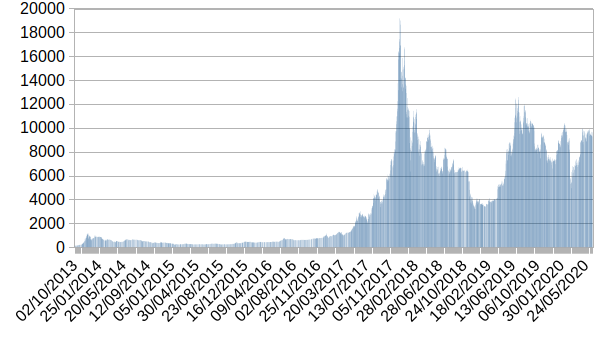
\includegraphics[width=\linewidth]{Bitcoin_linear.png}
\caption{Valor de venda de uma Bitcoin (02/10/2013 - 24/05/2020).}\label{bitcoinlinear}
\end{figure}

Esse gráfico traz informações importantes, mas não é adequado todas as questões. Muitas vezes o investidor está interessado no ganho relativo (crescimento percentual) que a moeda (ou ação) teve e não no valor absoluto da função. Nesse sentido, colocar o gráfico em escala logarítmica ajuda entender os períodos de maior crescimento (ou queda) relativo, devido a observação \textit{Crescimento proporcional com logaritmos}. Vejamos o valor das Bitcoins na escala logarítmica então. 

\begin{figure}[H]
\centering

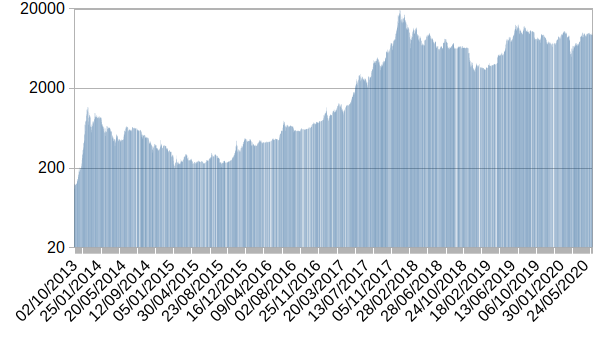
\includegraphics[width=\linewidth]{Bitcoin_log.png}

\caption{Valor de venda de uma Bitcoin (escala logarítmica).}\label{bitcoinlog}
\end{figure}

O gráfico mostra, então, que o crescimento proporcional no início da venda da Bitcoin foi maior do que o crescimento proporcional no pico de valor em dezembro de 2017 / janeiro de 2018, o que não estava aparente no gráfico linear.
\end{example}


\explore{O logaritmo natural}


A função $e^x$, onde $e=2{,}718\cdots$ número de Euler, já foi estudada no capítulo sobre a função exponencial e ela é a função exponencial preferencial nas ciências naturais e na engenharia. Isso ocorre pois ela é a linguagem natural do crescimento. A preferência do logaritmo natural está presente nas próprias calculadoras, que normalmente só calculam logaritmos em base 10, que escrevemos $\log_{10}$ ou $\log$, e a base $e$, que escrevemos $\log_e$ ou $\ln x$.

\begin{observation}{A função logarítmica natural.}
A função logarítmica de base $e$, $\log_e: \mathbb{R}^+_* \to \mathbb{R}$, é chamada de \textbf{função logarítmica natural} e denotada por $\ln$. Assim como para as outras bases, as funções $\ln x$ e $e^x$ são inversas, de modo que, para quaisquer reais $x$ e $y$, com $x>0$, temos:
\begin{align*}
& e^{\ln x} = x;
& \ln e^y = y.
\end{align*}
\end{observation}

Devido a base $e$ expressar o crescimento de forma mais natural, é muito comum que quaisquer exponenciais sejam escritas em termos da função $e^x$ utilizando a seguinte técnica, ilustrada para a função exponencial $5^x$:
$$
5^x = e^{\ln 5^x} = e^{x\ln 5} \approx e^{1{,}609 x},
$$
onde utilizamos a aproximação com três casas decimais para $\ln 5$.

\begin{task}{Na base $e$.}
Escreva as seguintes funções exponenciais utilizando a base $e$, como no exemplo acima, utilizando aproximações com três casas decimais de precisão para os logaritmos naturais.
\begin{enumerate}
\item $f(x)=3^x$;
\item $g(x)=10^x$;
\item $f(x)=75^x$.
\end{enumerate}
\end{task}


\arrange{Decaimento radioativo}

\begin{figure}[H]
\centering

\begin{tikzpicture}
    % Carbono
    \coordinate (dv) at (0,0);
    \coordinate (base) at (50pt,0pt);
    \coordinate (height) at (0pt,50pt);
    \coordinate (diag) at ($(base)+(height)$);
    \fill[rounded corners=2pt, grafite] ($(dv)-.5*(diag)$) rectangle +(diag); 
    \node[white] at (dv) {\sffamily\Huge \textbf{C}};
    \node[white, inner sep=2pt] (dvtext) at ($(dv)-.5*(height)$) [anchor=south] {\sffamily\small Carbono};
    \node[white, inner sep=2pt] (dvnum) at ($(dv)+.5*(height)-.5*(base)$) [anchor=north west] {\sffamily\small 6};
    \node[white, inner sep=2pt] (dvnum) at ($(dv)+.5*(height)+.5*(base)$) [anchor=north east] {\sffamily\small 12};
\end{tikzpicture}
\end{figure}


Os elementos químicos são catalogados na tabela periódica. A figura acima ilustra o \textbf{isótopo mais comum do carbono}, o Carbono-12, que tem número atômico 6 (e, assim, 6 prótons) e número de massa 12, tendo 6 nêutrons. Contudo nem todos os átomos de carbono são iguais, alguns têm nêutrons em excesso ou em falta. Classificamos os átomos em isótopos de acordo com o número de nêutrons que eles têm. Um isótopo importante do carbono é o Carbono-14, que é utilizado na datação de objetos antigos.

O Carbono-14 é um isótopo instável, e pode, espontaneamente, emitir radiação (e transformar-se em um átomo de nitrogênio). Esse processo natural é chamado de decaimento radioativo e diferentes isótopos decaem à taxas (velocidades) diferentes.

\begin{observation}{A meia vida de isótopos radioativos.}
A \textbf{meia vida} de um isótopo radioativo é o tempo necessário para que a metade dos átomos daquele isótopo em uma amostra decaia. Alguns exemplos de meia-vida de isótopos:

\begin{table}[H]
\centering

\begin{tabu} to \textwidth{|l|r|}
\hline
\tcolor{Oxigênio-19} & 26,5 s\\
\hline
\tcolor{Césio-137} & 30 anos\\
\hline
\tcolor{Carbono-14} & 5730 anos \\
\hline
\tcolor{Urânio-235} & 703.800.000 anos\\
\hline
\end{tabu}

\caption{Meias-vidas de alguns isótopos radioativos (aproximações).}
\end{table}

\end{observation}

\begin{example}{Decaimento do Carbono-14.}
O decaimento do Carbono-14 é utilizado para determinar a idade de tecidos orgânicos mortos e, por isso, é muito importante em diversas áreas da ciência. Vamos considerar uma amostra com 100g de Carbono-14 e determinar quanto tempo seria necessário para que sobrasse apenas 10g de Carbono-14 na amostra.

Como perdemos metade da massa a cada meia-vida, teremos as seguintes quantidades de Carbono-14 após determinado número de anos

\begin{table}[H]
\centering

\begin{tabu} to \textwidth{|r|l|}
\hline
\thead
Anos & Carbono-14 \\
\hline 
$0$ & $100$g \\
\hline
$5.730$ & $50$g \\
\hline
$11.460$ & $25$g \\
\hline
$17.190$ & $12{,}5$g \\
\hline
$22.930$ & $6{,}25$g \\
\hline 
$28.650$ & $3{,}125$g \\
\hline
\end{tabu}
\caption{Quantidade de Carbono-14 restante.}
\end{table}

Vemos que a quantidade cai exponencialmente a cada 5.730 anos. Assim, poderíamos escrever uma expressão para a quantidade de Carbono-14 como
$$
Q(t) = 100\times \left(\frac{1}{2}\right)^{t/5730} = 100\times e^{t\frac{\ln 1/2}{5730}} = 100\times e^{-t\frac{0{,}693}{5730}},
$$
onde escrevemos a função exponencial de base $e$ por ser a mais utilizada nesse contexto. Assim o tempo necessário para termos 10g seria
\begin{align*}
& 0{,}1=e^{-t\frac{0{,}693}{5730}}\\
\Longrightarrow& -t\frac{0{,}693}{5730} = \ln 0{,}1\\
\Longrightarrow& t \approx \frac{5730}{0{,}693}2,302 = 19.033{,}852
\end{align*}
\end{example}


\begin{task}{Meia vida biológica.}
A meia vida de um fármaco é o tempo necessário para a concentração plasmática dele cair pela metade em um organismo. Esse conceito serve para estimarmos qual a concentração de determinado medicamento no organismo. O antibiótico Amoxicilina tem meia vida biológica de 61,3 minutos. Vejamos a seguinte situação: um paciente de 75Kg recebe uma dose do medicamento de 500mg. Uma pessoa com esse peso tem cerca de 5 litros de sangue (a quantidade exata pode variar de pessoa para pessoa). Supondo que o medicamento foi completamente dissolvido e distribuído uniformemente no sangue, teríamos a concentração plasmática do medicamento igual a 500/5000 = 0,1 mg/ml. Escreva uma função exponencial de base $e$ para descrever concentração plasmática (em mg/ml) após $t$ minutos. Utilize a função encontrada para determinar quanto tempo levará para a concentração cair abaixo de 0,005 mg/ml. 
\end{task}


\explore{Escalas logarítmicas.}

\section{Escala Richter}

Ocorrem milhares de eventos sísmicos todo o dia no planeta Terra, mas a grande maioria deles é muito fraca para ser percebida pelos seres humanos. A magnitude de um evento sísmico varia muito, por isso tais eventos são classificados em escalas logarítmicas. Uma escala bastante famosa para medir os abalos é a escala Richter (mas que não é tão utilizada hoje em dia).

A escala Richter\footnote{Desenvolvida por Charles Richter e Beno Gutenberg} utiliza as amplitudes da das ondas registradas por sismógrafos para expressar a magnitude local de um evento sísmico, onde está localizado o sismógrafo.
\begin{figure}[!h]
\centering

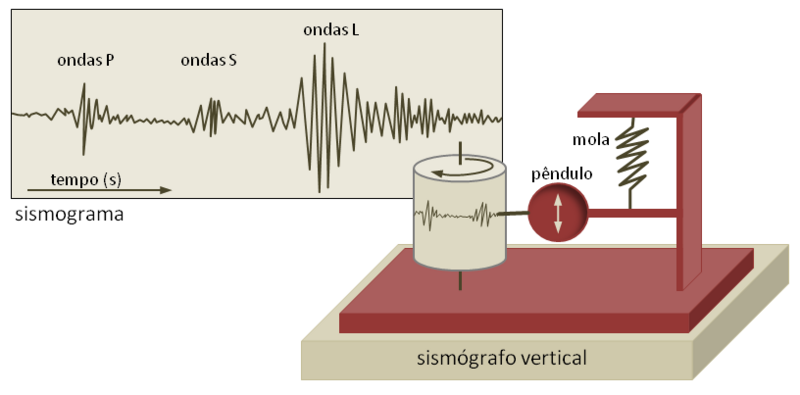
\includegraphics[width=0.8\linewidth]{Sismografo.png}

\caption{Um sismógrafo e o registro de um evento \\ Fonte: Casa das Ciências (\url{https://www.casadasciencias.org/}).}

\end{figure}

A Magnitude Local (ML) determinada pela escala Richter pode ser calculada por
$$
ML = \log_{10} A - \log A_0,
$$
onde $A$ é a maior amplitude de onda detectada pelo sismógrafo e $A_0$ é a magnitude do menor abalo registrável (na época de sua invenção), corrigida por um fator de escala, que depende da distância do sismógrafo à fonte do tremor.


\begin{example}{Comparando eventos (Escala Richter).}
Segundo a Wikipedia, a explosão na central nuclear de Chernobyl, em 1986, apresentou Magnitude Local $ML_{Ch} = 3{,}67$, enquanto o Sismo da Costa Rica, em 2009, apresentou Magnitude Local de $ML_{CR}=6{,}2$. Podemos comparar os eventos calculando a razão entre as amplitudes registradas através da diferença entre as Magnitudes Locais:
\begin{align*}
&6{,}2-3{,}67 = \log_{10} A_{CR} - \log A_0 - (\log_{10} A_{Ch} - \log A_0)\\
\implies & 2{,}53 = \log_{10} A_{CR} - \log_{10} A_{Ch} = \log_{10} \left(\frac{A_{CR}}{A_{Ch}}\right)\\
\implies & \left(\frac{A_{CR}}{A_{Ch}}\right) = 10^{2{,}53} \approx 338{,}84.
\end{align*} 
Assim o Sismo da Costa Rica registrou amplitudes 338 vezes maiores do que a explosão nuclear de Chernobyl.
\end{example}

A escala Richter apresenta distorções para eventos de grande ($>6{,}5$) intensidade e não é utilizada para grandes eventos sísmicos atualmente.

\section{Magnitude de Momento Sísmico}

Uma escala bastante utilizada atualmente é a escala de Magnitude ds Momento Sísmico ($MMS$), que também é uma escala logarítmica e utiliza o Momento Sísmico ($M_0$) para estimar a magnitude de um evento através da equação
$$
M_{\mathrm {w} }={\frac{2}{3}}\log_{10}\left(M_{0}\right)-10,7
$$

\begin{example}{Comparando eventos (MMS).}
Segundo a Wikipedia, a explosão da Tsar Bomba (maior artefato nuclear já detonado), detonada em 1961, atingiu Magnitude de Momento Sísmico $M_{\mathrm w} = 8{,}3$, enquanto o impacto do meteoro que, presumidamente, causou a extinção dos dinossauros, atingiu Magnitude de Momento Sísmico $N_{\mathrm w} = 13{,}0$. Podemos comparar os eventos calculando a razão entre os Momentos Sísmicos $M_T$ e $M_D$, respectivamente, calculando a diferença entre as Magnitudes de Momento Sísmicos:
\begin{align*}
&13{,}0-8{,}3 = {\frac{2}{3}}\log_{10}\left(M_{D}\right)-10,7-\left( {\frac{2}{3}}\log_{10}\left(M_{T}\right)-10,7\right)\\
\implies & 4{,}7 = {\frac{2}{3}}\left(\log_{10}\left(M_{D}\right)-\log_{10}\left(M_{T}\right)\right) =  {\frac{2}{3}}\log_{10}\left(\frac{M_D}{M_T}\right)\\
\implies & \left(\frac{M_D}{M_T}\right) = 10^{7{,}05} \approx 11.220.184{,}54.
\end{align*} 
Assim o impacto do meteoro gerou um Momento Sísmico mais de 11 milhões de vezes maior do que o Momento Sísmico do maior artefato nuclear já detonado pela espécie humana. 
\end{example}

\section{pH}

O pH, às vezes chamado de potencial de Ionização, é uma escala utilizada para medir a acidez ou basicidade de uma solução aquosa. Substâncias ácidas tem o pH menor do que 7 e substâncias básica tem o pH maior do que 7. A água pura tem pH=7 e é considerada neutra. Vejamos alguns exemplos dos valores de pH  para substâncias comuns:


\begin{table}[H]
\centering
\setlength\tabulinesep{2pt}

\begin{tabu} to \textwidth{|l|l|}
\hline
\thead
Substância & pH \\
\hline
Ácido de bateria & < 1,0\\
\hline
Suco gástrico	& 1,0 - 3,0\\
\hline
Sumo de limão	& 2,2 - 2,4\\
\hline
Refrigerante tipo cola	& 2,5\\
\hline
Vinagre	& 2,4-3,4\\
\hline
Sumo de laranja ou maçã	& 3,5\\
\hline
Cervejas	& 4,0 - 5,0\\
\hline
Café	& 5,0\\
\hline
Chá &	5,5\\
\hline
Chuva ácida	& < 5,6\\
\hline
Leite	& 6,3 - 6,6\\
\hline
Água pura	&7,0\\
\hline 
Saliva humana	& 6,5 - 7,5\\
\hline
Sangue humano	& 7,35 - 7,45\\
\hline
Água do mar	& 8,0\\
\hline 
Sabonete de mão	& 9,0 - 10,0\\
\hline
Amoníaco &	11,5\\
\hline
Hidróxido de sódio (soda cáustica)&	13,5\\
\hline
\end{tabu}

\caption{Alguns valores comuns de pH.\\Fonte: Dados da Wikipedia-pH (\url{pt.wikipedia.org/wiki/PH}).}
\end{table}

O pH é definido a partir da atividade dos íons de hidrônio ($a_{H^+}$), medida em mols/L, na solução, que pode ser medida com um aparelho eletrônico. Então o pH é definido como menos o logaritmo da atividade dos íons de hidrônio:
$$
pH = - \log_{10} a_{H^+}
$$


\begin{task}{\,pH no vestibular.}
[UDESC 2009] “Chuva ácida” é um termo que se refere à precipitação, a partir da
atmosfera, de chuva com quantidades de ácidos nítricos e sulfúrico maiores que o
normal. Os precursores da chuva ácida vem tanto de fontes naturais, tais como vulcões
e vegetação em decomposição, quanto de processos industriais, principalmente
emissões de dióxido de enxofre e óxidos de nitrogênio resultantes da queima de
combustíveis fósseis. O pH da água da chuva considerado normal é de 5,5 (devido
à presença de ácido carbônico proveniente da solubilização de dióxido de carbono).
Um químico monitorando uma região altamente industrializada observou que o pH da
água da chuva era igual a 4,5. Considerando que a acidez está relacionada com a
concentração de $H_3O^+$, é correto afirmar que a água com pH 4,5 era:
\begin{itemize}
\item[(A)] duas vezes mais básica que o normal.
\item[(B)] duas vezes mais ácida que o normal.
\item[(C)] dez vezes mais básica que o normal.
\item[(D)] dez vezes mais ácida que o normal.
\item[(E)] cem vezes mais ácida que o normal.
\end{itemize}
\end{task}



\exercise


\begin{enumerate}

\item \label{Exer1} Segundo o gráfico abaixo, quantas vezes a massa corporal de um besouro é maior do que a massa corporal de uma formiga? E qual seria a razão entre as massas de um coelho e de um besouro? E entre as massas da formiga e do coelho?

\begin{figure}[H]
\centering

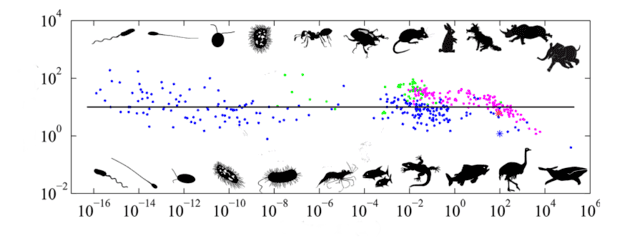
\includegraphics[width=\linewidth]{Massa.png}
\caption{{Distribuição de massas, em quilogramas no eixo horizontal, e velocidades, em comprimentos do ser vivo por segundo no eixo horizontal.} \\ Fonte: Meyer-Verneta (2015)
% \cite{Mayer15}
}
\end{figure}


\item \label{Exer2} Para doenças infecciosas, em seus estágios iniciais, é esperado que o aumento no número de casos seja proporcional ao número de contaminados (em estágios posteriores essa tendência diminuí pois há menos pessoas suscetíveis disponíveis para a contaminação). Os gráficos abaixo mostram o desenvolvimento  do número de casos da Covid-19 no mundo em escala linear e logarítmica. Observando os gráficos, houve maior crescimento relativo no número de casos entre as datas de 22 de janeiro e 10 de fevereiro ou entre as datas de 30 de abril e 20 de maio? Qual dos gráficos identifica melhor a situação?

\begin{figure}[H]
\centering

\includegraphics[width=.9\linewidth]{World_linear.png}
\caption{Total de casos confirmados da Covid-19 no mundo (linear)\\
Fonte: \textit{Our World in Data} (\url{ourworldindata.org}).}
\end{figure}

\begin{figure}[H]
\centering

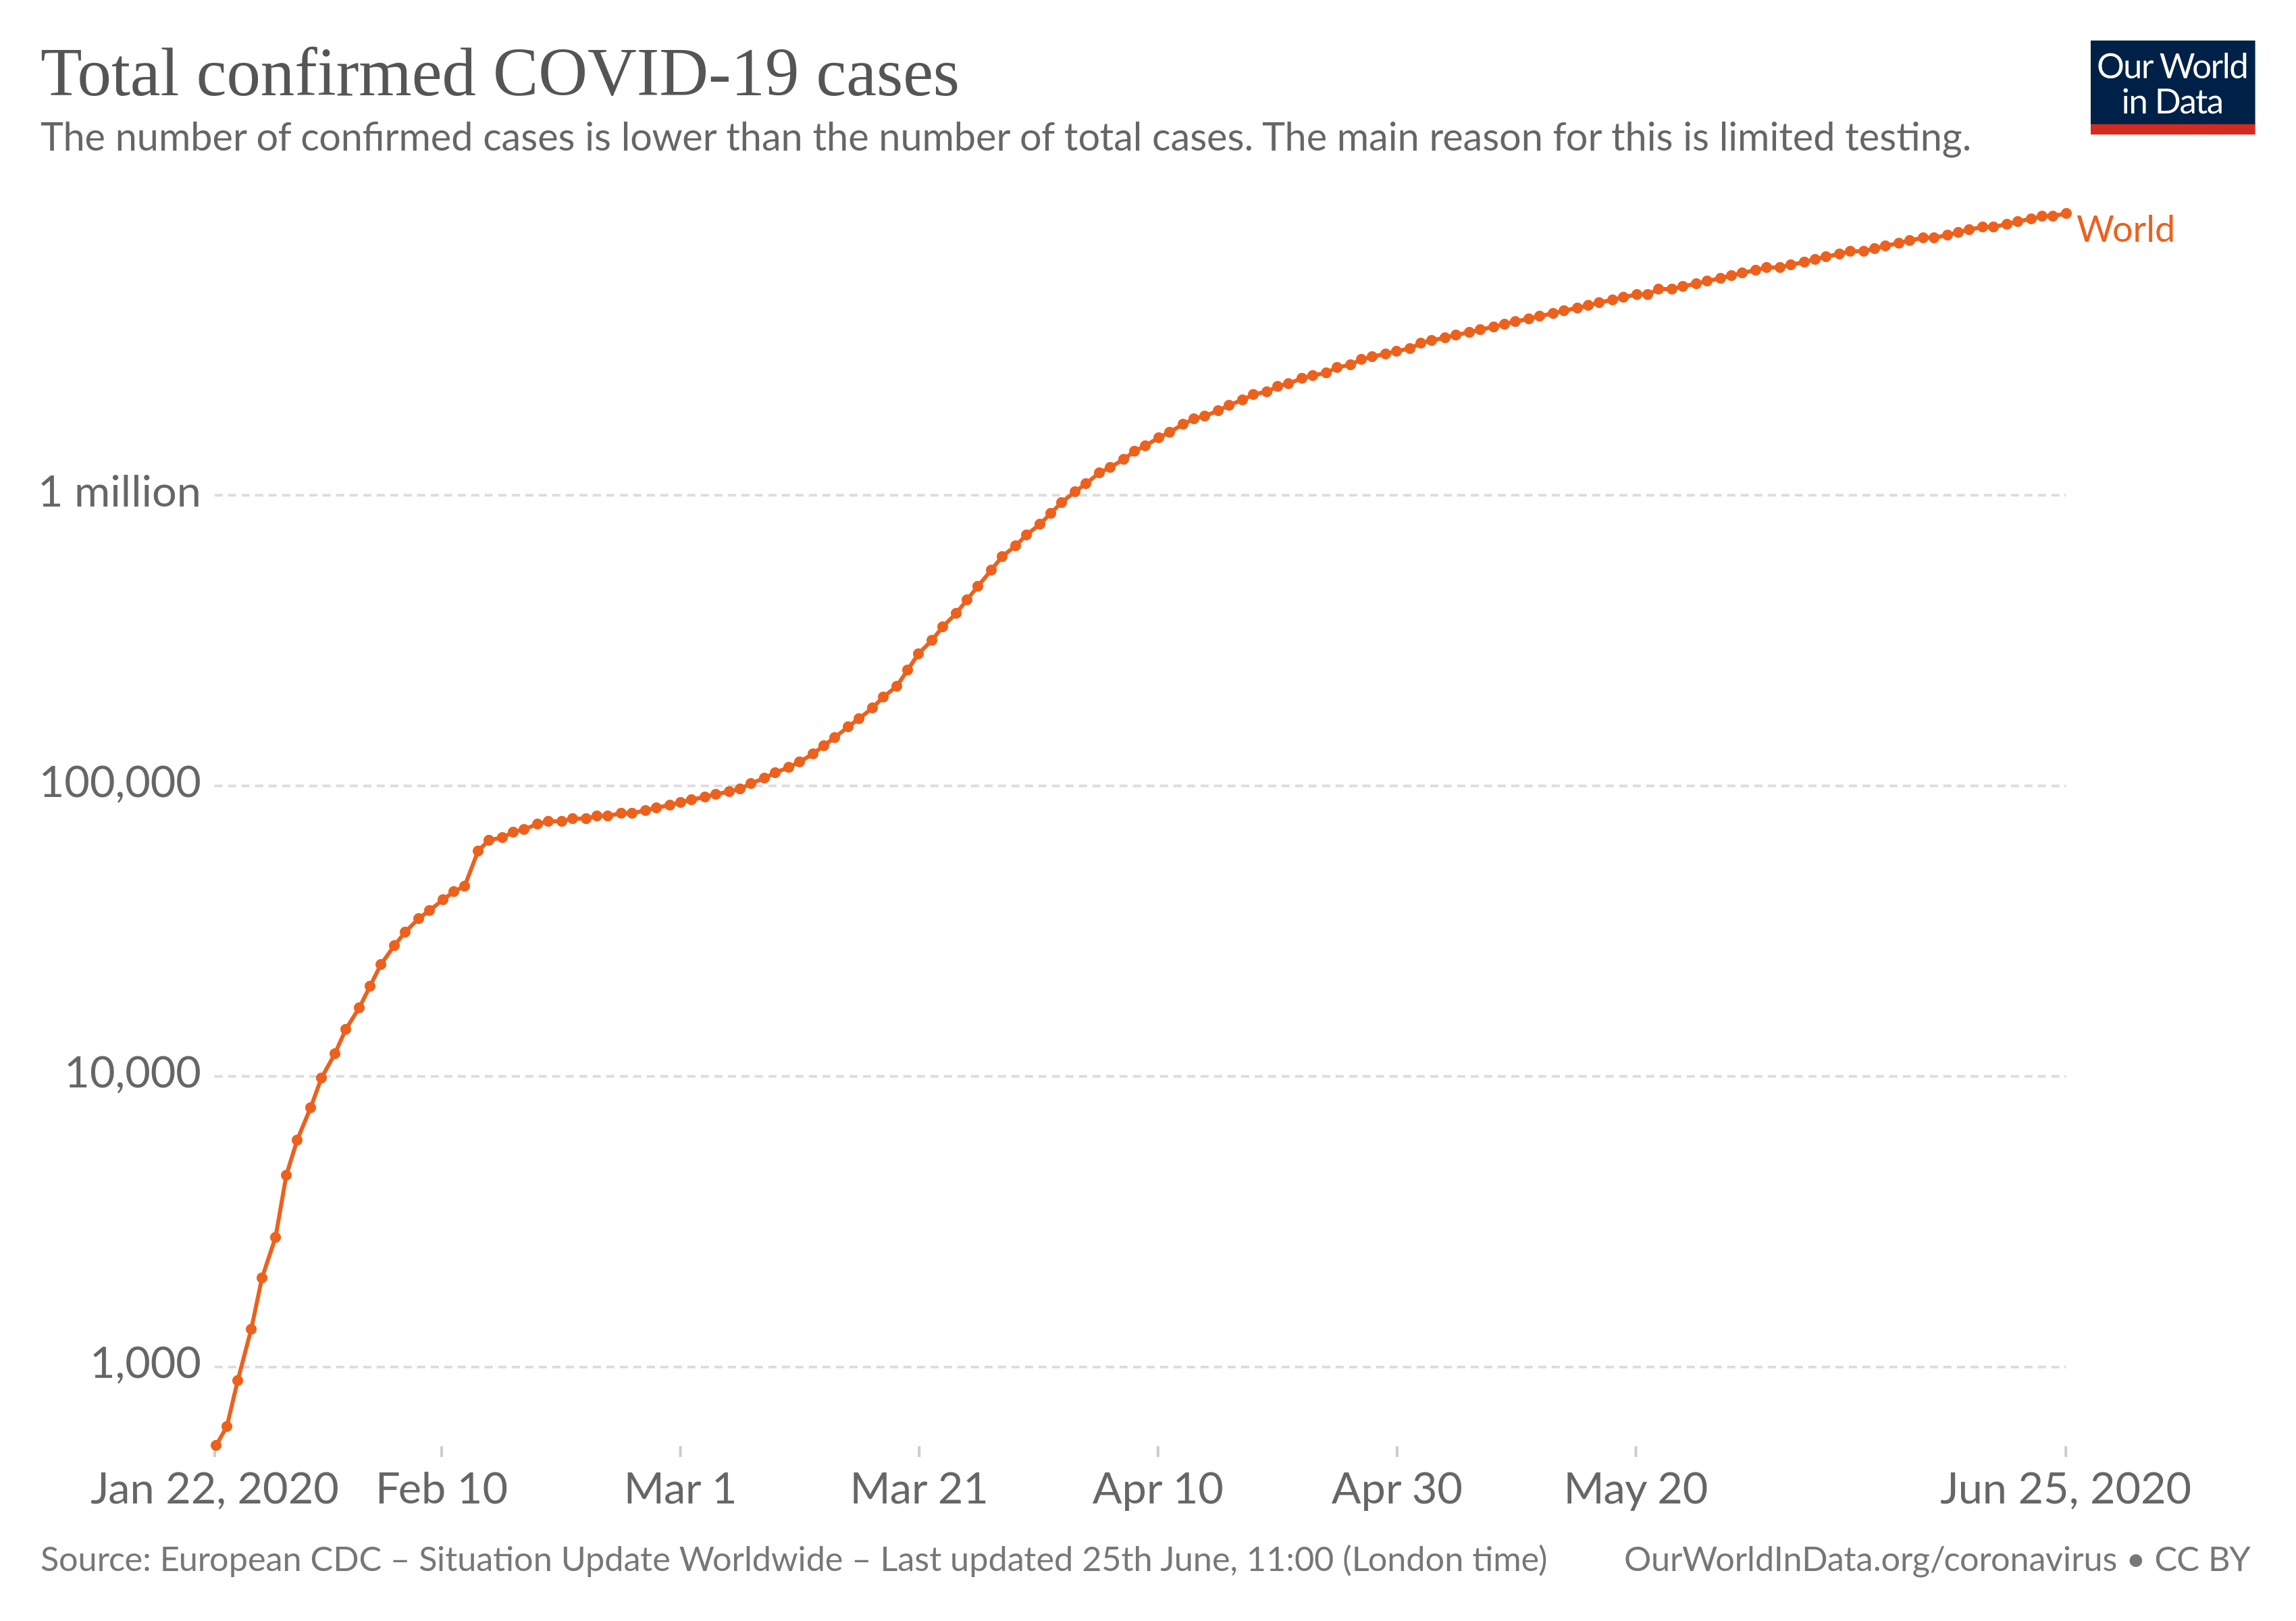
\includegraphics[width=.9\linewidth]{World_log.png}\vspace{3mm}\\
\caption{Total de casos confirmados da Covid-19 no mundo (log)\\
Fonte: \textit{Our World in Data} (\url{ourworldindata.org}).}
\end{figure}


\item \label{Exer3} Observando as figuras \ref{bitcoinlinear} e \ref{bitcoinlog}, o crescimento percentual do valor da Bitcoin foi maior entre as datas de 02/10/2013 e 25/01/2014 ou entre 05/11/2017 e 28/02/2018? Como isso pode ser observado nos gráficos?


\item \label{Exer4} (ENEM 2019) Um jardineiro cultiva plantas ornamentais e as coloca à venda quando estas atingem 30 centímetros de altura. Esse jardineiro estudou o crescimento de suas plantas, em função do tempo, e deduziu uma fórmula que calcula a altura em função do tempo, a partir do momento em que a planta brota do solo até o momento em que ela atinge sua altura máxima de 40 centímetros. A fórmula é $h = 5\log_2 (t + 1)$, em que t é o tempo contado em dia e h, a altura da planta em centímetro. A partir do momento em que uma dessas plantas é colocada à venda, em quanto tempo, em dia, ela alcançará sua altura máxima?
\begin{enumerate}
\item 63
\item 96
\item 128
\item 192
\item 255
\end{enumerate}


\item \label{Exer5} (PEIES/2008) Segundo o IBOPE, o número de internautas no Brasil chegou, em março de 2007, a 16,3 milhões de pessoas. Em 2000, esse número era aproximadamente 5 milhões. Suponha que a função N(t), que representa o número de internautas\footnote{Em uma situação real, só é possível esperar crescimento exponencial enquanto o total de internautas é muito menor do que a população total.} (em milhões) em função do tempo $t$ (em ano), possa ser expressa por $N(t) = 5(1{,}184)^t$, onde $t = 0$ representa o ano de 2000, $t = 1$, o ano de 2001 e assim por diante. Então, de acordo com esse modelo, o número de internautas atingirá 50 milhões: (dado $\log 1{,}184 = 0{,}073$)
\begin{enumerate}
\item entre 2008 e 2009;
\item entre 2009 e 2010;
\item em março de 2010;
\item entre 2013 e 2014;
\item somente a partir de 2015.
\end{enumerate}



\item \label{Exer6}

O pH de uma solução é definido por pH$=-\log_{10}(H^+)$  em que $H^+$ é a concentração de hidrogênio em íons-grama por litro de solução. Determine o pH de uma solução tal que $H^+ = 10^{-5}$.


   
\item \label{Exer7} (USF Geral 2015) Terremoto é o termo popular usado para os grandes sismos, sendo que para os pequenos é comum 
usar 
abalo sísmico ou tremor de terra. A escala Richter, também conhecida como escala de magnitude local (ML), atribui um 
número único para quantificar o nível de energia liberada por um sismo. É uma escala logarítmica de base 10, obtida 
calculando o logaritmo da amplitude horizontal combinada (amplitude sísmica) do maior deslocamento a partir do zero em 
um tipo particular de sismógrafo. 

A fórmula utilizada é $ML = \log(A) - \log (A_0)$, em que: 

A = amplitude máxima medida no sismógrafo. 

$A_0$ = uma amplitude de referência. 

Com base nas informações, analise as proposições: 

I. Para um terremoto de magnitude 7, temos que $A_0 = 7A$. 

II. Para um terremoto de magnitude 4 temos que $\frac{A}{A_0}=10^{-4}$ .
 
III. Um terremoto de magnitude 7 produz efeitos 10 vezes maior do que um terremoto de magnitude 6. 

Assinale a correta.
\begin{enumerate}
    \item Apenas a proposição I é verdadeira.
    \item Apenas as proposições I e II são verdadeiras
	\item Apenas as proposições II e III são verdadeiras.
	\item Apenas a proposição II é verdadeira.
	\item Apenas a proposição III é verdadeira.
\end{enumerate}


\item \label{Exer8} (Enem 2011) A Escala de Magnitude de Momento (abreviada como MMS e denotada como $M_w$), introduzida em 1979 por Thomas 
Haks e Hiroo Kanamori, substituiu a Escala de Richter para medir a magnitude dos terremotos em termos de energia 
liberada. Menos conhecida pelo público, a MMS é, no entanto, a escala usada para estimar as magnitudes de todos os 
grandes terremotos da atualidade. Assim como a escala Richter, a MMS é uma escala logarítmica. 
$M_w$ e $M_0$ se relacionam pela fórmula:
$$
M_w = - 10,7 + \frac{2}{3}\log_{ 10 }(M_0).
$$
Onde $M_0$ é o momento sísmico (usualmente estimado a partir dos registros de movimento da superfície, através dos 
sismogramas), cuja unidade é o dina x cm. O terremoto de Kobe, acontecido no dia 17 de janeiro de 1995, foi um dos 
terremotos que causaram maior impacto no Japão e na comunidade científica internacional. Teve magnitude $M_w = 7,3$.
\footnote{U.S. Geological Survey. Historic Earthquakes.
Disponível em: \url{http://earthquake.usgs.gov}. 
Acesso em: 1º maio 2010 (adaptado).
U.S. Geological Survey.USGS Earthquake Magnitude Policy.
Disponível em: \url{http://earthquake.usgs.gov}. 
Acesso em: 1º maio 2010 (adaptado).}

Mostrando que é possível determinar a medida por meio de conhecimentos matemáticos, qual foi o momento sísmico $M_0$ do 
terremoto de Kobe (em dina$\cdot$cm)?

\begin{enumerate}
    \item $10^{-5,10}$
    \item $10^{-5,73}$
    \item $10^{12,00}$
    \item $10^{21,65}$
    \item $10^{27,00}$
\end{enumerate}


\item \label{Exer9} (UFSCar-SP) A altura média do tronco de certa espécie de árvore, que se destina a produção de madeira, evolui, 
desde que é plantada, segundo o seguinte modelo matemático:
$$
h(t): 1,5 + \log_3 (t+1),
$$ com $h(t)$ em metros e $t$ em anos. 
Se uma dessas árvores foi cortada quando seu tronco atingiu 3,5m de altura, o tempo (em anos) transcorrido da 
plantação 
ao corte foi de:
\begin{enumerate}
    \item 9
    \item 8
    \item 5
    \item 4
    \item 2
\end{enumerate}


\item \label{Exer10} (UnB-DF) Estima-se que 1 350 $m^2$ de terra sejam necessários para fornecer alimento para uma pessoa. Admite-se, 
também, que há $30 \times 1 350$ bilhões de $m^2$ de terra arável no mundo e que, portanto, uma população máxima de 30 
bilhões de pessoas pode ser sustentada, se não forem exploradas outras fontes de alimento. A população mundial, no 
início de 1987, foi estimada em 5 bilhões de habitantes. Considerando que a população continua a crescer, a uma taxa de 
2{\%} ao ano, e usando as aproximações $\ln(1{,}02) = 0{,}02$;  $\ln(2) = 0{,}70$ e  $\ln(3) = 1{,}10$, determine em quantos anos, 
a partir de 1987, a Terra teria a máxima população que poderia ser sustentada.




\item \label{Exer11} (UFMG) O pH de uma solução aquosa é definido pela expressão pH $= -\log [H^+]$, em que $[H^+]$ indica a concentração, em 
mol/L, de íons de hidrogênio na solução e $\log$, o logaritmo na base 10.
Ao analisar uma determinada solução, um pesquisador verificou que, nela, a concentração de íons de hidrogênio era $[H^+] 
= 5,4\cdot 10^{-8} mol/L$. Para calcular o pH dessa solução, ele usou os valores aproximados de $0{,}30$, para $\log 2$, e de $0{,}48$, para  $\log 3$.
Então, o valor que o pesquisador obteve para o pH dessa solução foi:
\begin{enumerate}
    \item  7,26 
    \item 7,32 
    \item  7,58
    \item 7,74
\end{enumerate}

\item \label{Exer12} (ENEM - 2016) Uma liga metálica sai do forno a uma temperatura de $3.000^o C$ e diminui 1{\%} de sua temperatura a 
cada 
30 min. Use 0,477 como aproximação para $\log (3)$ e 1,041 como aproximação para $\log (11)$. O tempo decorrido, em horas, até 
que a liga atinja $30^0 C$ é mais próximo de
\begin{enumerate}
    \item 22.
    \item 50.
    \item 100.
    \item 200.
    \item 400.
\end{enumerate}


\item \label{Exer13} (PUC-SP) A energia nuclear, derivada de isótopos radiativos, pode ser usada em veículos espaciais para fornecer 
potência. Fontes de energia nuclear perdem potência gradualmente, no decorrer do tempo. Isso pode ser descrito pela 
função exponencial
$$
P=P_0 e^{-\frac{t}{250}}
$$
na qual P é a potência instantânea, em watts, de radioisótopos de um veículo espacial; $P_0$ é a 
potência inicial do veículo; t é o intervalo de tempo, em dias, a partir de $t_0 = 0$; e é a base do sistema de 
logaritmos neperianos. Nessas condições, quantos dias são necessários, aproximadamente, para que a potência de um 
veículo espacial se reduza à quarta parte da potência inicial? (Dado: $\ln 2 = 0{,}693$)
 \begin{enumerate}
     \item 336
     \item 338
     \item 340
     \item 342
     \item 346
 \end{enumerate}

\item \label{Exer14} (UNESP-SP) O altímetro dos aviões é um instrumento que mede a pressão atmosférica e transforma esse resultado em 
altitude. Suponha que a altitude $h$ acima do nível do mar, em quilômetros, detectada pelo altímetro de um avião seja 
dada, em função da pressão atmosférica $p$, em atm, por
$$
h(p)=20\log_{10}\left(\frac{1}{p}\right).
$$
Num determinado instante, a pressão atmosférica medida pelo altímetro era $0{,}4$atm. Considerando a aproximação 
$\log_{10} 2 =0{,}3$, a altitude $h$ do avião nesse instante, em quilômetros, era de

\begin{enumerate}
\item 5. 
\item 8. 
\item 9.
\item 11.
\item 12.
\end{enumerate}


%\item (Unicamp - SP) As populações de duas cidades, $A$ e $B$, são dadas em milhares de habitantes pelas funções 
%$A(t)=\log_8 (t+1)^6$ e $B(t) =\log_2 (4t+4)$, em que a variável $t$ representa o tempo em anos.
%
%\begin{enumerate}
%\item Qual é a população de cada uma das cidades nos instantes $t=1$ e $t=7$? 
%\item Após certo instante $t$, a população de uma dessas cidades é sempre maior do que a da outra. Determine esse 
%instante $t$ e especifique a cidade cuja população é maior após esse instante.
%\end{enumerate}

\item \label{Exer15} (UFPR - 2017) A probabilidade de se vencer uma partida de certo jogo é de 10{\%}. Quantas partidas devem ser 
jogadas em sequência para que a probabilidade de que haja vitória em pelo menos uma delas seja superior a 99{\%}? Se 
necessário, use $\log(3) = 0{,}477$.
\begin{enumerate}
\item 10.
\item 20.
\item 22.
\item 30.
\item 44.

\end{enumerate}

\end{enumerate}

\pagebreak
\know{sem ferramentas de cálculo...}


Os logaritmos foram inventados pelo matemático escocês John Napier (1550 - 1617) e desenvolvidos na base 10 pelo matemático inglês Henry Briggs (1561 - 1630). Eles desenvolveram os logaritmos para facilitar as cálculos de multiplicação\footnote{A seção \textit{Para saber +: a régua de cálculo} traz mais detalhes sobre essa utilização dos logaritmos}, que eram muito laboriosos e passíveis de erro em uma época que não haviam computadores. Para isso eles precisavam de tabelas extensas, que enchiam livros inteiros, com os valores aproximados de muitos logaritmos em alguma base.


\begin{figure}[H]
\centering
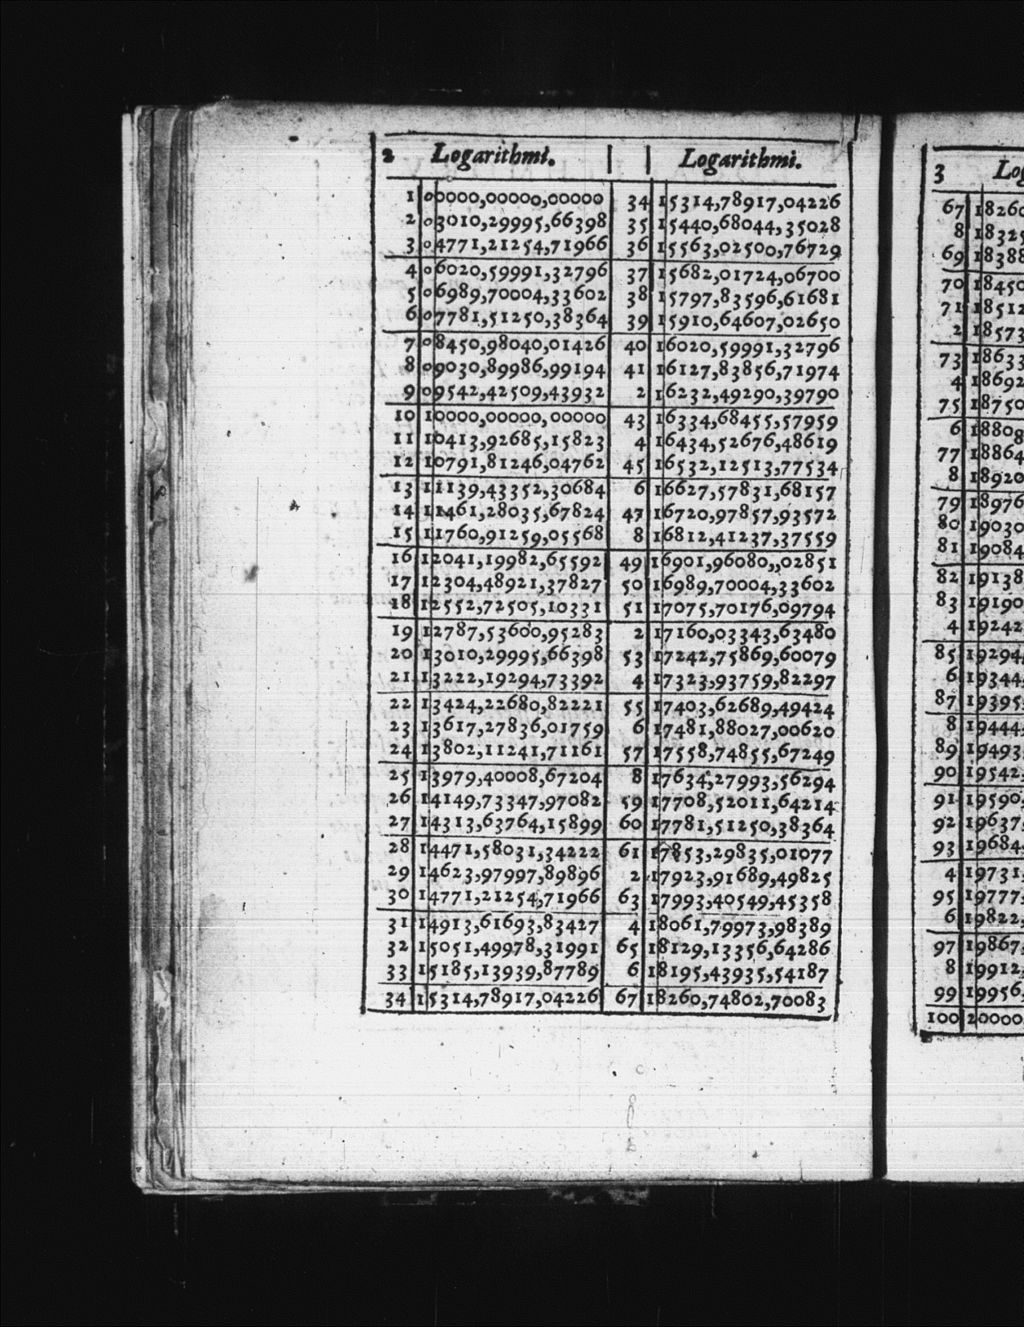
\includegraphics[height=80mm]{Logarithmorum_Chilias_Prima_page_0-67.jpg}%Figura de domínio público
\caption{Uma página do \textit{Logarithmorum Chilias Prima} de Henry Briggs, publicado em 1617, com aproximações dos logarimos em base 10 dos números inteiros de 0 à 67 com precisão de 14 casas decimais.}
\end{figure}


Vamos ilustrar como calcular $\log_2 3$ manualmente utilizando o método da bissecção. Esse método já era utilizado para calcular aproximações\footnote{Outro uso importante é para calcular raízes ou zeros de funções.} antes da invenção dos computadores, mas ainda é bastante utilizado na computação.



\begin{observation}{O método da bissecção}
Para aplicarmos o método da bissecção, tomamos uma aproximação superior e outra inferior para o número buscado, encontrando assim um intervalo no qual temos certeza em que a solução se encontra. Então tomamos o ponto médio desse intervalo como a próxima aproximação e testamos se ele é superior ou inferior ao número buscado, então basta substituirmos o respectivo extremo do intervalo por ele. Repetindo esse processo obtemos aproximações cada vez melhores para o número buscado.
\end{observation}


O $\log_2 3$ é o expoente em que precisamos elevar $2$ para obter $3$, ou seja $2^{\log_2 3} = 3$, assim precisamos encontrar expoentes tais que 2 elevado a esses expoentes se aproxima cada vez mais de 3.  Podemos iniciar nossas tentativas com os expoentes $1$ e $2$. De fato $2^1=2<3$ e $2^2 = 4>3$, junto ao fato que as potências de 2 crescem quando crescem os expoentes, temos que $1<\log_2 3 < 2$. Para aplicar o método, escolhemos então, inicialmente, as aproximações inferior $i=1$ e superior $s=2$.

Tomamos, então a metade do intervalo $(1,2)$ como uma primeira aproximação $x=(1+2)/2 = 3/2$.

\begin{figure}[H]
\centering

\begin{tikzpicture}[scale=1.5]
\draw[black] (1,0) -- (6,0);
\draw[black] (2,-0.1) -- (2,0.1);
\draw[black] (3.5,-0.1) -- (3.5,0.1);
\draw[black] (5,-0.1) -- (5,0.1);
\node[black] at (2,-0.5) {$i=1$};
\node[black] at (5,-0.5) {$s=2$};
\node[black] at (3.5,-0.5) {$x=1{,}5$};
\draw[penvinho,->,thick] (4.5,0.5) .. controls(4.1,0.3) .. (3.9,0.05);
\node[penvinho] at (4.9,0.5) {$\log_2 3$};
\end{tikzpicture}
\end{figure}


Agora precisamos verificar se $x = 3/2$ é uma aproximação superior ou inferior e fazemos isso verificando se $2^{3/2}$ é maior ou menor do que $3$, que é o mesmo que comparar $2^3=8$ com $3^2=9$, pois a raiz quadrada é uma função crescente. Como $2^3 < 3^2$, temos que $2^{3/2}<3$ e $3/2<\log_2 3$, novamente pelo fato das potências de 2 crescerem quando crescem os expoentes. Assim a nova aproximação inferior passa a ser $i=3/2$ e aproximação superior continua sendo $s=2$.

Tomamos, então a metade do intervalo $(3/2, 2)$ como uma segunda aproximação $x=(3/2+2)/2 = 7/4$. 

\begin{figure}[H]
\centering

\begin{tikzpicture}[scale=1.5]
\draw[black] (1,0) -- (6,0);
\draw[black] (2,-0.1) -- (2,0.1);
\draw[black] (3.5,-0.1) -- (3.5,0.1);
\draw[black] (5,-0.1) -- (5,0.1);
\node[black] at (2,-0.5) {$i=1{,}5$};
\node[black] at (5,-0.5) {$s=2$};
\node[black] at (3.5,-0.5) {$x=1{,}75$};
\draw[penvinho,->,thick] (4.5,0.5) .. controls(4.1,0.3) .. (3.9,0.05);
\node[penvinho] at (4.9,0.5) {$\log_2 3$};
\end{tikzpicture}
\end{figure}

Agora precisamos verificar se $2^{7/4}$ é maior ou menor do que $3$, que é o mesmo que comparar $2^7=128$ com $3^4=81$, pois a raiz quarta é uma função crescente. Como $2^7 > 3^4$, temos que $2^{7/4}>\log_2 3$ e $7/4$ é uma aproximação superior. 

Tomamos, então a metade do intervalo $(3/2, 7/4)$ como uma terceira aproximação $x=(3/2+7/4)/2 = 13/8$.

\begin{figure}[H]
\centering

\begin{tikzpicture}[scale=1.5]
\draw[black] (1,0) -- (6,0);
\draw[black] (2,-0.1) -- (2,0.1);
\draw[black] (3.5,-0.1) -- (3.5,0.1);
\draw[black] (5,-0.1) -- (5,0.1);
\node[black] at (2,-0.5) {$i=1{,}5$};
\node[black] at (5,-0.5) {$s=1{,}75$};
\node[black] at (3.5,-0.5) {$x=1{,}625$};
\draw[penvinho,->,thick] (4.5,0.5) .. controls(4.1,0.3) .. (3.9,0.05);
\node[penvinho] at (4.9,0.5) {$\log_2 3$};
\end{tikzpicture}
\end{figure}


Agora precisamos verificar se $2^{13/8}$ é maior ou menor do que $3$. Para fazer isso comparamos $2^{13/8}$ com $3$, que é o mesmo que comparar $2^{13}=8192$ com $3^8=6561$. Como $2^{13} > 3^8$, temos que $2^{13/8}>\log_2 3$ e $13/8$ é uma aproximação superior. 

Podemos continuar esse processo quantas vezes desejarmos, mas vamos parar com o intervalo $(3/2,13/8)$ e tomar o ponto médio dele $x=(3/2+13/8)/2=25/16$ como aproximação.

\begin{figure}[H]
\centering

\begin{tikzpicture}[scale=1.5]
\draw[black] (1,0) -- (6,0);
\draw[black] (2,-0.1) -- (2,0.1);
\draw[black] (3.5,-0.1) -- (3.5,0.1);
\draw[black] (5,-0.1) -- (5,0.1);
\node[black] at (2,-0.5) {$i=1{,}5$};
\node[black] at (5,-0.5) {$s=1{,}625$};
\node[black] at (3.5,-0.5) {$x=1{,}5625$};
\draw[penvinho,->,thick] (4.5,0.5) .. controls(4.1,0.3) .. (3.9,0.05);
\node[penvinho] at (4.9,0.5) {$\log_2 3$};
\draw [decorate,decoration={brace,amplitude=10pt},xshift=0.2,yshift=0pt]
(2,0) -- (3.5,0);
\node [black] at (2.75,0.4) {\footnotesize $0{,}0625$};
\end{tikzpicture}
\end{figure}



A aproximação para o logaritmo está boa? Pelo fato de $3/2 < \log_2 3 < 13/8$, temos certeza que $\log_2 3$ está no intervalo $(3/2,13/8)$. Contudo nossa aproximação está no centro do intervalo e à uma distância menor do que a metade do seu comprimento ($(13/8-3/2)/2= 1/16 = 0,0625$) de qualquer ponto do intervalo, inclusive $\log_2 3$. Assim garantimos que o erro em nossa aproximação é menor do que $0{,}0625$.

\begin{task}{cálculo do $\log_2 5$}
Utilize o método da bissecção para calcular $\log_2 5$ com erro menor do que $0,25$. 
\end{task}


\know{Logaritmos com a régua de cálculo}

Antes do surgimento e popularização das calculadoras digitais, era muito laborioso efetuar todas as operações de multiplicação e divisão necessárias em muitas atividades, como no controle de estoques, na contabilidade, no cálculo de impostos e em cálculos astronômicos (principalmente ligados à navegação). Os logaritmos foram inventados para facilitar esses cálculos. Frequentemente as operações de multiplicação e divisão são consideradas triviais, 
contudo para números razoavelmente longos é fácil cometer erros nos cálculos:

\begin{task}{Multiplicação manual}
Calcule, sem a utilização de equipamentos eletrônicos,
$$
19683 \times 2187.
$$
Verifique, com a ajuda de uma calculadora, se obteve a resposta correta.
\end{task}

Erros são bastante comuns em cálculos de multiplicação e representavam um problema sério quando os cálculos eram necessários e 
não havia nenhum 
meio eletrônico que permitisse a verificação deles. A respeito deste problema, o escocês considerado o inventor dos 
logaritmos: John Nepier \footnote{Também conhecido como John Naper ou  Ioannes Neper na versão latinizada de seu 
nome.}, 
escreveu (tradução livre) em sua obra de 1614:
\begin{quote}
Dado que nada (caros amadores apaixonados pela Matemática) é tão desagradável à prática matemática 
(freando e retardando os especialistas no cálculo) quanto as multiplicações, as divisões e as extrações de raízes 
quadradas ou cúbicas de números grandes que, além do incômodo devido ao seu tamanho, induzem a diversos erros 
perigosos; 
como consequência, eu me dediquei a procurar por que meios seguros e cômodos poderia me livrar destas 
dificuldades.

\raggedleft \textit{John Napier - Mirifici logarithmorum canonis descriptio} 
\end{quote}

O cálculo realizado acima pode ser feito de modo muito mais rápido se tivermos uma tabela com os valores das potências de $3$ e levarmos em conta que:
\begin{itemize}
 \item $3^5=2187$,
  \item $3^7=19683$,
   \item $19683 \times 2187 = 3^5 \times 3^7 = 3^{12} = 43046721$.
\end{itemize}


Assim, podemos utilizar a Tabela \ref{potencias2_log} para fazer cálculos de multiplicação ou divisão, somando ou subtraindo  os logaritmos e localizando o resultado correspondente a soma, ao invés de multiplicar explicitamente:
\begin{itemize}
 \item $5 \times 4 \approx 2^{2{,}32} \times 2^2 = 2^{2{,}32 + 2} = 2^{4{,}32} \approx 20$;
 \item $3 \times 5 \approx 2^{1{,}58} \times 2^{2{,}32} = 2^{1{,}58 + 2{,}32} = 2^{3{,}9} \approx 15$;
 \item $3 \times 9 \approx 2^{1{,}58} \times 2^{3{,}16} = 2^{1{,}58+3{,}16} = 2^{4{,}74} \approx 27$.
  \item $20 \div 4 \approx 2^{4{,}32} \div 2^{2} = 2^{4,32-2} = 2^{2{,}32} \approx 5$.
 \end{itemize}

Apesar dos cálculos da soma dos expoentes não darem, necessariamente, os valores exatos que temos na 
tabela, buscamos o que melhor se aproxima. Fazemos isso pois sabemos que o produto de dois naturais é novamente um 
natural e temos todos os naturais até 30 listados na tabela.


Napier escreveu um livro inteiro de logaritmos tabelados para consulta e utilização em cálculos. Henri Briggs, um dos pais dos logaritmos, publicou um livro\footnote{Há uma foto de uma página do livro no \textit{Para saber +: sem ferramentas de cálculo...}} com todos os logaritmos em base 10 dos números naturais de $1$ à $20000$. Mas, não é muito prático carregarmos uma longa tabela por aí. Para lidar com esse problema, William Oughtred  (1574 – 1660) inventou réguas de cálculo.

\begin{figure}
\centering
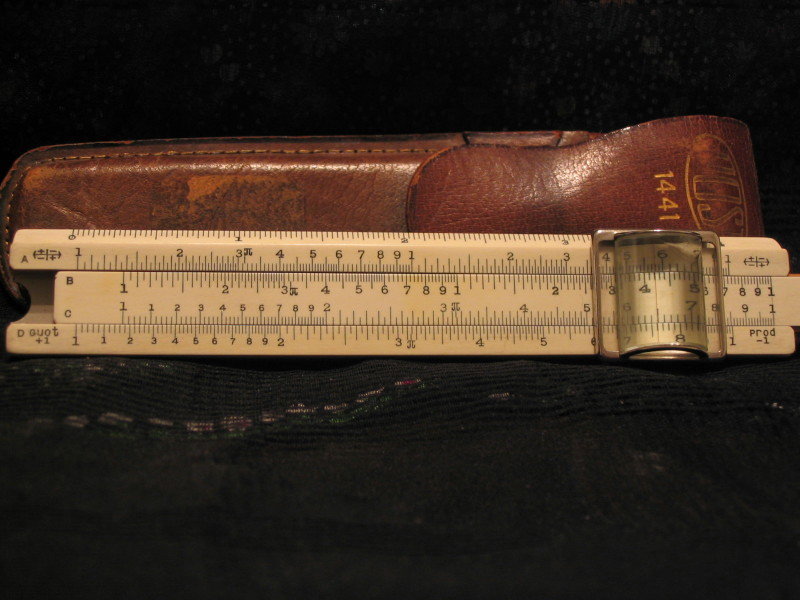
\includegraphics[width=0.5\linewidth]{Figuras/Reguadecalculo}\\

\caption{Uma régua de cálculo \\ Fonte: Slide Rule em Flickr / Usuário: The Last Cookie}
\end{figure}

A régua linear de Oughtred efetuava multiplicações e divisões com duas escalas logarítmicas, fazendo as partes da régua deslizarem uma sobre a outra. A régua de cálculo, com suas variantes, foi, durante mais de 300  anos, uma ferramenta indispensável para engenheiros e cientistas, era um presente dado de pais para filhos ao final do 
ginásio. Ela aprimorada por diversos cientistas e engenheiros até chegar em sua versão atual. Estudaremos uma régua de cálculo simplificada nas atividades seguintes.


\textbf{A Régua de Cálculo}

Na régua aritmética ou linear, o comprimento 1cm corresponde ao número 1, o comprimento 2 cm corresponde ao número 2 e assim sucessivamente. Na régua de cálculo logarítmica de base 2, o número 1 corresponde ao comprimento do logaritmo de 1 em base 2, o número 2 corresponde ao comprimento do logaritmo de 2 e assim por diante. A Figura \ref{Reguas} 
ilustra uma régua de cálculo formada por duas partes, cada uma com uma linha central e uma escala linear, ambas na cor 
cinza, e uma escala logarítmica na cor preta. Note que na escala logarítmica marcamos, por exemplo, o número 3 à distância 1,59 do 
ponto inicial da escala, o número 1, pois $\log_2 3 \approx 1{,}59$.

\begin{figure}[H]
\centering

\begin{tikzpicture}[scale=2]
 \fill [white] (1.7,1.3) rectangle (6.25,2.3);
\draw (1.7,1.3)--(6.25,1.3);
 \draw (1.7,2.3)--(6.25,2.3);
 \draw (1.7,1.3)--(1.7,2.3);
 \draw (6.25,1.3)--(6.25,2.3);
 \draw (2,1.4)--(2,1.3);
 \node at (2,1.55) {1};
  \draw (3,1.4)--(3,1.3);
 \node at (3,1.55) {2};
 \draw[blue,thick] (3,1.55) circle (0.15cm);
  \draw[purple,thick,->] (3,1.25) -- (3,1);
   \draw (3.62,1.4)--(3.62,1.3);
 \node at (3.62,1.55) {3};
 \draw[blue,thick] (3.62,1.55) circle (0.15cm);
   \draw[purple,thick,->] (3.62,1.25) -- (3.62,1);
   \draw (4,1.4)--(4,1.3);
 \node at (4,1.55) {4};
   \draw (4.33,1.4)--(4.33,1.3);
 \node at (4.33,1.55) {5};
   \draw (4.59,1.4)--(4.59,1.3);
 \node at (4.59,1.55) {6};
   \draw (4.82,1.4)--(4.82,1.3);
 \node at (4.82,1.55) {7};
   \draw (5,1.4)--(5,1.3);
 \node at (5,1.55) {8};
   \draw (5.18,1.4)--(5.18,1.3);
 \node at (5.18,1.55) {9};
   \draw (5.33,1.4)--(5.33,1.3);
 \node at (5.33,1.55) {10};
    \draw (5.59,1.4)--(5.59,1.3);
 \node at (5.59,1.55) {12};
    \draw (5.81,1.4)--(5.81,1.3);
 \node at (5.81,1.55) {14};
    \draw (6,1.4)--(6,1.3);
 \node at (6,1.55) {16};
   \draw[gray] (1.7,1.8)--(6.25,1.8);
   \draw[gray] (2,1.9)--(2,1.8);
 \node[gray] at (2,2.05) {0};
    \draw[gray] (3,1.9)--(3,1.8);
 \node[gray] at (3,2.05) {1};
    \draw[gray] (4,1.9)--(4,1.8);
 \node[gray] at (4,2.05) {2};
    \draw[gray] (5,1.9)--(5,1.8);
 \node[gray] at (5,2.05) {3};
    \draw[gray] (6,1.9)--(6,1.8);
 \node[gray] at (6,2.05) {4};
  \fill [white] (-0.3,0) rectangle (4.25,1);
 \draw (-0.3,0)--(4.25,0);
 \draw (-0.3,1)--(4.25,1);
 \draw (-0.3,0)--(-0.3,1);
 \draw (4.25,0)--(4.25,1);
 \draw (0,0.9)--(0,1);
 \node at (0,0.75) {1};
  \draw (1,0.9)--(1,1);
 \node at (1,0.75) {2};
   \draw (1.62,0.9)--(1.62,1);
 \node at (1.62,0.75) {3};
   \draw (2,0.9)--(2,1);
 \node at (2,0.75) {4};
\draw[blue,thick] (2,0.75) circle (0.15cm);
 \draw (2.33,0.9)--(2.33,1);
 \node at (2.33,0.75) {5};
   \draw (2.59,0.9)--(2.59,1);
 \node at (2.59,0.75) {6};
   \draw (2.82,0.9)--(2.82,1);
 \node at (2.82,0.75) {7};
   \draw (3,0.9)--(3,1);
 \node at (3,0.75) {8};
     \draw[purple,thick] (2.88,0.63) rectangle (3.12,0.87);
   \draw (3.18,0.9)--(3.18,1);
 \node at (3.18,0.75) {9};
   \draw (3.33,0.9)--(3.33,1);
 \node at (3.33,0.75) {10};
    \draw (3.59,0.9)--(3.59,1);
 \node at (3.59,0.75) {12};
      \draw[purple,thick] (3.47,0.63) rectangle (3.71,0.87);
    \draw (3.81,0.9)--(3.81,1);
 \node at (3.81,0.75) {14};
    \draw (4,0.9)--(4,1);
 \node at (4,0.75) {16};
  \draw[gray] (-0.3,0.5)--(4.25,0.5);
   \draw[gray] (0,0.4)--(0,0.5);
 \node[gray] at (0,0.25) {0};
    \draw[gray] (1,0.4)--(1,0.5);
 \node[gray] at (1,0.25) {1};
    \draw[gray] (2,0.4)--(2,0.5);
 \node[gray] at (2,0.25) {2};
    \draw[gray] (3,0.4)--(3,0.5);
 \node[gray] at (3,0.25) {3};
    \draw[gray] (4,0.4)--(4,0.5);
 \node[gray] at (4,0.25) {4};
 \end{tikzpicture}

\caption{Uma régua de cálculo e sua utilização calculando 4x2 e 4x3. \\ Fonte: Logaritmos e a régua de cálculo, Pedrosa \& Adames.}
\label{Reguas}
\end{figure}

Podemos utilizar as réguas de cálculo para fazer multiplicações ou divisões.

Para multiplicar $a \times b$, basta colocar as duas metades da régua uma sobre a outra, como na figura, colocando o número 1 da metade 
superior da régua sobre $a$. O resultado estará então abaixo de $b$. Como ilustra a Figura \ref{Reguas} nas 
multiplicações 4x2 e 4x3.


\begin{figure}[H]
\centering

\begin{tikzpicture}[scale=2]
 \fill [white] (0.69,1.3) rectangle (5.24,2.3);
\draw (0.69,1.3)--(5.24,1.3);
 \draw (0.69,2.3)--(5.24,2.3);
 \draw (0.69,1.3)--(0.69,2.3);
 \draw (5.24,1.3)--(5.24,2.3);
 \draw (0.99,1.4)--(0.99,1.3);
 \node at (0.99,1.55) {1};
  \draw (1.99,1.4)--(1.99,1.3);
 \node at (1.99,1.55) {2};
   \draw (2.61,1.4)--(2.61,1.3);
 \node at (2.61,1.55) {3};
   \draw[purple,thick,->] (0.99,1.25) -- (0.99,1);
   \draw (2.99,1.4)--(2.99,1.3);
 \node at (2.99,1.55) {4};
   \draw (3.32,1.4)--(3.32,1.3);
 \node at (3.32,1.55) {5};
   \draw (3.58,1.4)--(3.58,1.3);
 \node at (3.58,1.55) {6};
   \draw (3.81,1.4)--(3.81,1.3);
 \node at (3.81,1.55) {7};
  \draw[blue,thick] (3.81,1.55) circle (0.15cm);
   \draw (3.99,1.4)--(3.99,1.3);
 \node at (3.99,1.55) {8};
   \draw (4.17,1.4)--(4.17,1.3);
 \node at (4.17,1.55) {9};
   \draw (4.32,1.4)--(4.32,1.3);
 \node at (4.32,1.55) {10};
    \draw (4.58,1.4)--(4.58,1.3);
 \node at (4.58,1.55) {12};
    \draw (4.8,1.4)--(4.8,1.3);
 \node at (4.8,1.55) {14};
    \draw (4.99,1.4)--(4.99,1.3);
 \node at (4.99,1.55) {16};
   \draw[gray] (0.69,1.8)--(5.24,1.8);
   \draw[gray] (0.99,1.9)--(0.99,1.8);
 \node[gray] at (0.99,2.05) {0};
    \draw[gray] (1.99,1.9)--(1.99,1.8);
 \node[gray] at (1.99,2.05) {1};
    \draw[gray] (2.99,1.9)--(2.99,1.8);
 \node[gray] at (2.99,2.05) {2};
    \draw[gray] (3.99,1.9)--(3.99,1.8);
 \node[gray] at (3.99,2.05) {3};
    \draw[gray] (4.99,1.9)--(4.99,1.8);
 \node[gray] at (4.99,2.05) {4};
  \fill [white] (-0.3,0) rectangle (4.25,1);
 \draw (-0.3,0)--(4.25,0);
 \draw (-0.3,1)--(4.25,1);
 \draw (-0.3,0)--(-0.3,1);
 \draw (4.25,0)--(4.25,1);
 \draw (0,0.9)--(0,1);
 \node at (0,0.75) {1};
  \draw (1,0.9)--(1,1);
 \node at (1,0.75) {2};
 \draw[purple,thick] (0.88,0.63) rectangle (1.12,0.87);
   \draw (1.62,0.9)--(1.62,1);
 \node at (1.62,0.75) {3};
   \draw (2,0.9)--(2,1);
 \node at (2,0.75) {4};
 \draw (2.33,0.9)--(2.33,1);
 \node at (2.33,0.75) {5};
   \draw (2.59,0.9)--(2.59,1);
 \node at (2.59,0.75) {6};
   \draw (2.82,0.9)--(2.82,1);
 \node at (2.82,0.75) {7};
   \draw (3,0.9)--(3,1);
 \node at (3,0.75) {8};
   \draw (3.18,0.9)--(3.18,1);
 \node at (3.18,0.75) {9};
   \draw (3.33,0.9)--(3.33,1);
 \node at (3.33,0.75) {10};
    \draw (3.59,0.9)--(3.59,1);
 \node at (3.59,0.75) {12};
    \draw (3.81,0.9)--(3.81,1);
 \node at (3.81,0.75) {14};
  \draw[blue,thick] (3.81,0.75) circle (0.15cm);
    \draw (4,0.9)--(4,1);
 \node at (4,0.75) {16};
  \draw[gray] (-0.3,0.5)--(4.25,0.5);
   \draw[gray] (0,0.4)--(0,0.5);
 \node[gray] at (0,0.25) {0};
    \draw[gray] (1,0.4)--(1,0.5);
 \node[gray] at (1,0.25) {1};
    \draw[gray] (2,0.4)--(2,0.5);
 \node[gray] at (2,0.25) {2};
    \draw[gray] (3,0.4)--(3,0.5);
 \node[gray] at (3,0.25) {3};
    \draw[gray] (4,0.4)--(4,0.5);
 \node[gray] at (4,0.25) {4};
 \end{tikzpicture}

\captionof{figure}{Uma régua de cálculo utilizada para calcular $14 \div 7$.}\label{Reguas}
\end{figure}


Para dividir $a / b$, basta colocar as duas metades da régua uma sobre a outra, como na figura, colocando o número $b$ da metade 
superior da régua sobre $a$. O resultado estará então abaixo do número $1$. Como pode ser visto no resultado de $14 \div 7$, que está abaixo do número $1$.

Isso funciona pois ao colocarmos as réguas assim, estamos adicionando ou  subtraindo os comprimentos dos logaritmos dos respectivos números (na escala linear em cinza claro).

Por fim ainda temos o problema que a base dois cresce muito rapidamente. Para resolver isso podemos tomar uma que seja bem próxima de 1 e um pouco maior.

Produzimos réguas de cálculo, que estão no final do capítulo, utilizando a base $x = 10^{1/50}\approx 1{,}04713$, de modo que $\log_{x}100=100$. As graduações na régua correspondem aos logaritmos em base $x$ dos números de 0 a 10 com uma casa decimal de precisão e dos números naturais de 11 até 100. A régua também contém uma escala linear e as posições dos números na escala logarítmica correspondem aos valores dos logaritmos daqueles números na base $x$. A Figura \ref{ReguaCalculo} ilustra a régua.

\begin{figure}[H]
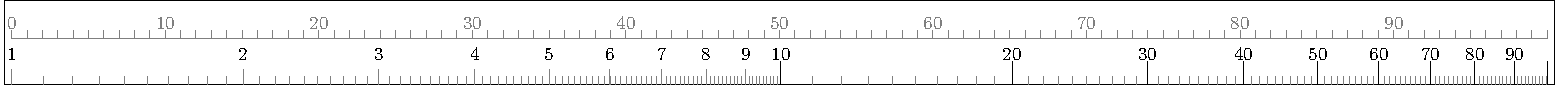
\includegraphics[width=\linewidth]{Figuras/Ruler1.pdf}

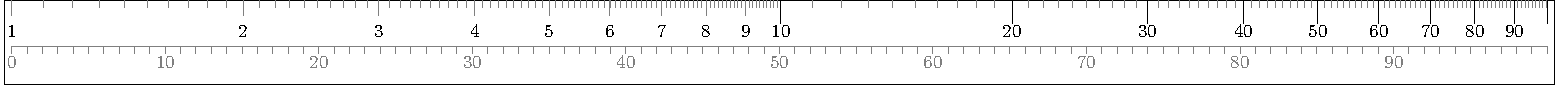
\includegraphics[width=\linewidth]{Figuras/Ruler2.pdf}

\caption{A régua de cálculo que acompanha este material. \\ Fonte: Logaritmos e a régua de cálculo, Pedrosa \& Adames.}\label{ReguaCalculo}
\end{figure}


\begin{task}{Cálculos com a régua}

Em pequenos grupos, vamos utilizar as réguas de cálculo para efetuar os seguintes cálculos:
\begin{enumerate}
 \item 9 x 7. %\textcolor{blue}{Basta colocar deslizar a metade superior de modo que o número 1 esteja sobre o número 9 da régua inferior e observar a resposta 63 abaixo do número 7 da metade superior.}
 \item 3,5 x 4.% \textcolor{blue}{Basta colocar deslizar a metade superior de modo que o número 1 esteja sobre o número 3,5 da régua inferior e observar a resposta 14 abaixo do número 4 da metade superior.}
 \item 2,8 x 2,5.% \textcolor{blue}{Basta colocar deslizar a metade superior de modo que o número 1 esteja sobre o número 2,8 da régua inferior e observar a resposta 7 abaixo do número 2,5 da metade superior.}
 \item 28 x 25.% \textcolor{blue}{Apesar dos números 28 e 25 estarem nas duas metades da régua, a posição onde estaria a reposta fica além do comprimento da régua, mas podemos realizar esse cálculo lembrando que $28 \times 25 = 2,8 \times 2,5 \times 10^2 = 7 \times 10^2 = 700$.}
 \item 3,2 x 3,1.% \textcolor{blue}{Ao aplicarmos o procedimento a resposta parece dar $9,9$. Isso ocorre pois há um limite para a escala de graduações escrita na régua, que tem precisão máxima de uma casa decimal para números menores do que 10 e precisão apenas da parte inteira para números maiores do que 10. A resposta exata seria 9,92 e a resposta 9,9 é uma aproximação para ela.}
\item 5,8 x 9,3.% \textcolor{blue}{A régua mostra a aproximação 54, que está bastante próxima da resposta exata 53,94.}
\item 583 x 93.% \textcolor{blue}{$583 \times 93 = 5,83 \times 9,3 \times 10^3 \approx 54 \times 10^3 = 54000$, que é uma aproximação para a resposta exata 54219.}
\item 78326 x 648.% \textcolor{blue}{$78326 \times 648 = 7,8326 \times 6,48 \times 10^6 \approx 51 \times 10^6 = 51000000$, que é uma aproximação para a resposta exata 50755248.}
\item 56 $\div$ 7.% \textcolor{blue}{Basta colocar deslizar a metade superior de modo que o número 7 esteja sobre o número 56 da régua inferior e observar a resposta 8 abaixo do número 1 da metade superior. Essa operação funciona pois a resposta para $56 \div 7$ é o número que multiplicado por 7 da 56, de modo que, ao colocarmos o número 7 sobre o número 56, o número abaixo do 1 é a resposta para $56 \div 7$.}
\item 58 $\div$ 4. %\textcolor{blue}{A régua mostra um valor entre 14 e 15, nesses casos podemos tomar a média entre eles, 14,5, que, por acaso, acaba coincidindo com a resposta exata.}
\item 93 $\div$ 5.% \textcolor{blue}{A régua mostra um valor entre 18 e 19, nesses casos podemos tomar a média entre eles, 18,5, que aproxima resposta exata 18,6.}
\item 476 $\div$ 93.% \textcolor{blue}{$476 \div 93 = 47,6 \div 9,3 \approx 5,1$, que é uma aproximação para a resposta dada pela calculadora 5,11827957 (que é apenas uma aproximação...).}
\item 7345 $\div$ 57.% \textcolor{blue}{$7345 \div 57 =73,45 \div 5,7 \times 10\approx 12,5 \times 10 = 125$, que é uma aproximação para a resposta dada pela calculadora 128,859649123 (que é apenas uma aproximação...).}
\end{enumerate}
\end{task}


\know{Ajustes de curvas}


Quando buscamos uma função para aproximar dados reais, podemos escolher que tipo de função parece mais adequada (o que pode ser um pouco subjetivo). Contudo, quando escolhemos um tipo de função, que valores escolhemos para os coeficientes dessa função? Por exemplo, se os dados parecem crescer como uma função logarítmica, qual deve ser a base? Para determinarmos essas constantes existem métodos mas que muitos programas de computador podem calcular automaticamente.

A caderneta de saúde abaixo traz as medidas (nas datas especificadas) da idade, do peso, da altura e do perímetro encefálico de uma criança.

\begin{figure}[H]
\centering

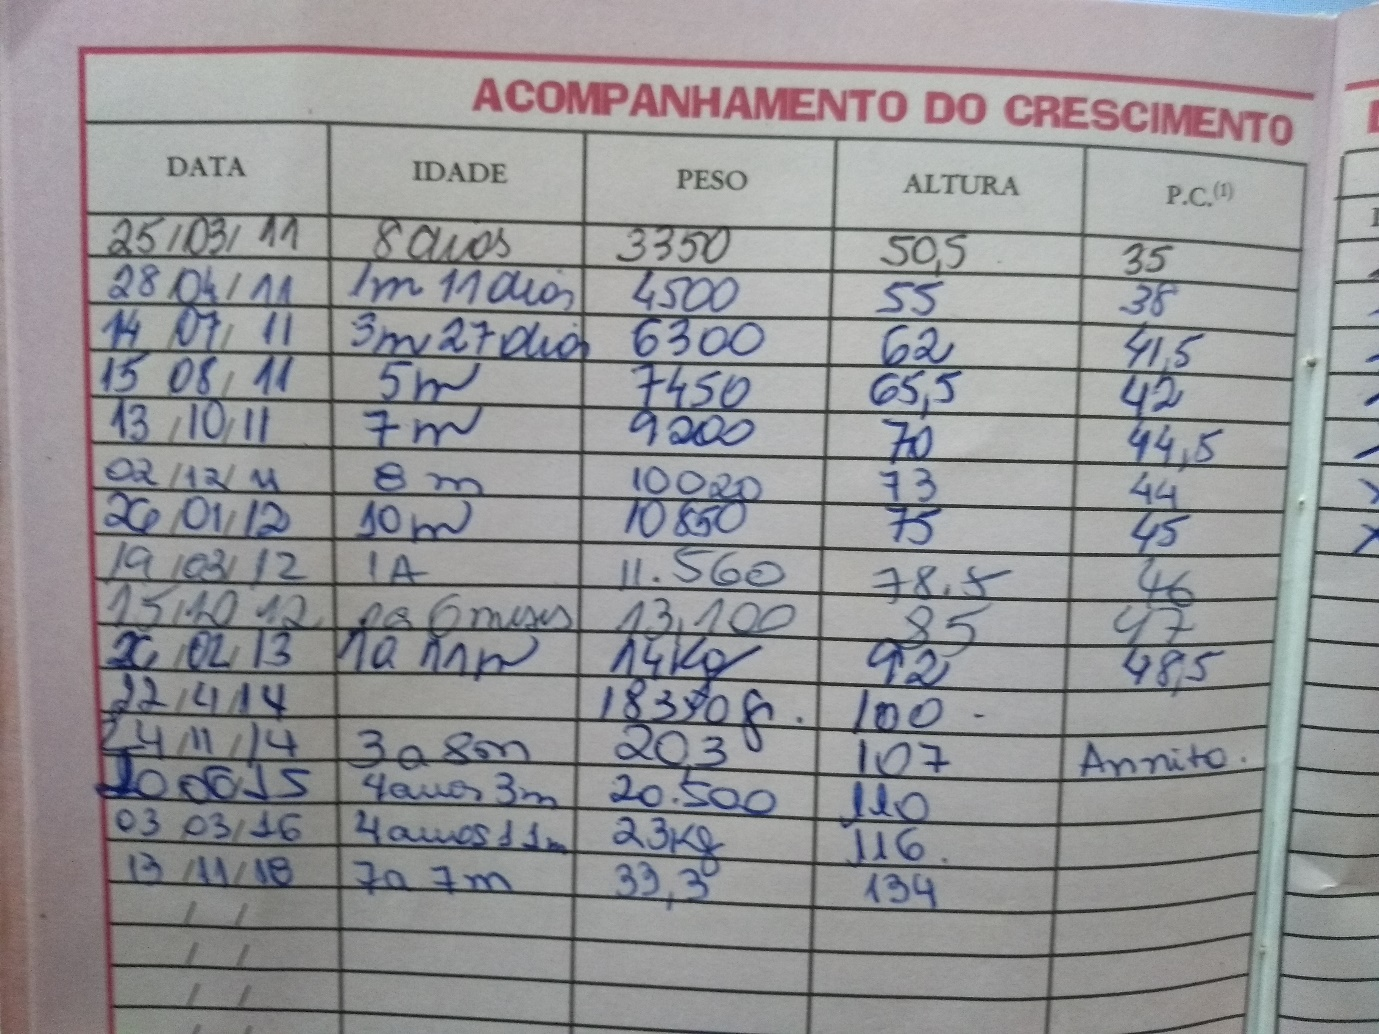
\includegraphics[width=0.8\linewidth]{Figuras/Caderneta.png}
\caption{Dados médicos na carteirinha de uma criança.}
\end{figure}

Anotamos os dados de idade e altura no GeoGebra, no endereço abaixo, e utilizamos as funções do programa para aproximar os dados utilizando curvas do tipo: exponencial, logarítmica, linear, logística, potência e polinomial.

\begin{figure}[H]
\centering


\includegraphics[width=.3\linewidth]{Figuras/QRcode_ajuste_curvas.png}

\url{https://www.geogebra.org/calculator/za7dq64a}
\end{figure}

\begin{reflection}
Vamos observar as funções mostradas pelo \textit{applet}. Quais dos ajustes parecem adequados ao crescimento da altura de uma pessoa? Quais levariam a previsões absurdas? Justifique os motivos que o levaram a realizar essas escolhas.
\end{reflection}


Foge dos objetivos desse material estudar em detalhes os métodos para encontrar as funções que \textit{melhor aproximam} os dados reais de cada um dos tipos. Contudo um dos métodos, chamado de \textit{regressão linear} está relacionado com os logaritmos.

\begin{knowledge}
A \textit{regressão linear} é um método utilizado com frequência para encontrar a função exponencial $y(x) =a \times b^x$ que melhor aproxima dados reais e consiste em aplicar logaritmos dos dois lados da equação, obtendo $\log y = \log a + x \log b$, que é uma equação linear do tipo $v = c + dx$, com $v = \log y$ e constantes $c=\log a$ e $d=\log b$. Essa nova equação pode ser ajustada aos logaritmos dos dados reais por um método chamado de mínimos quadrados, encontrando os melhores valores para $c$ e $d$ e, então, achamos $a= 10^c$ e $b=10^d$.
\end{knowledge}


\begin{task}{Regressão linear}
Utilizando os dados reais do número de casos nos Estados Unidos (fonte: \textit{Our World in Data}) entre 22/01/2020 e 21/03/2020, aplicamos regressão linear com uma ferramenta computacional para estimar o número de casos pela fórmula $f(t) = 0{,}000275279 \times 1{,}36451^t$, onde $t=0$ representa o dia 22/01 e $t= 59$ o dia 21/03. %(Ref: https://towardsdatascience.com/modeling-exponential-growth-49a2b6f22e1f)

Utilizando a fórmula, quantos dias seriam necessários para que a pandemia ultrapassasse 100.000 infectados naquele país?
\end{task}

Vamos comparar os dados obtidos pela fórmula com os dados reais.

\begin{table}[H]
\centering

\begin{tabu} to \textwidth{|*{7}{c|}}
\hline
\thead
& 22/03 & 23/03 & 24/03 & 25/03 & 26/03 & 27/03 \\
\hline
\tcolor{Dados reais} & 33.404 & 44.183 & 54.453 & 68.440 & 85.356 & 103.321\\
\hline
\tcolor{Previsão da função} & 34.544 & 47.136 & 64.317 & 87.762 & 119.752 & 163.403\\
\hline
\end{tabu}

\caption{Total de Casos nos E.U.A.}
\end{table}

Os valores são próximos no começo, mas começam a ficar distintos. Explicamos isso pelo fato da pandemia não se desenvolver livremente, mas há reações da população e das autoridades, como medidas sanitárias, que podem reduzir as taxas de infecção.


\know{Logaritmos e progressões}


Napier pensava nos logaritmos como produzidos por um movimento dinâmico. Traduzimos isso pensando em dois objetos $P$ e $Q$ movendo-se sobre duas semi-retas, um partindo da origem 0 e o outro do número 1, de modo que o  primeiro desloca-se com velocidade constante, mas o segundo tem velocidade proporcional a distância que ele está da origem da semi-reta. Assim, se tomarmos intervalos de tempo igualmente espaçados $T, 2T, 3T, 4T, \ldots$, obtemos posições distintas $P_1,P_2, \ldots$ e $Q_1,Q_2, \ldots$ para os dois objetos, como ilustra a Figura \ref{Movimento}.  

\begin{figure}
\centering

\begin{tikzpicture}[scale=1.5]
% \fill [white] (1.7,1.3) rectangle (6.25,2.3);
\draw [->](0,0)--(8,0);
\draw [->](0,-1)--(8,-1);
\draw (0,-0.05)--(0,0.05);
\node at (0,-0.2) {0};
\draw (0,-1.05)--(0,-0.95);
\node at (0,-1.2) {0};
\draw (1,-1.05)--(1,-0.95);
\node at (1,-1.2) {1};
\fill[purple,thick] (1,0) circle (0.7mm);
\node at (1,-0.2) {$P_1$};
\fill[purple,thick] (1.5,-1) circle (0.7mm);
\node at (1.5,-1.2) {$Q_1$};
\fill[purple,thick] (2,0) circle (0.7mm);
\node at (2,-0.2) {$P_2$};
\fill[purple,thick] (2.25,-1) circle (0.7mm);
\node at (2.25,-1.2) {$Q_2$};
\fill[purple,thick] (3,0) circle (0.7mm);
\node at (3,-0.2) {$P_3$};
\fill[purple,thick] (3.375,-1) circle (0.7mm);
\node at (3.375,-1.2) {$Q_3$};
\fill[purple,thick] (4,0) circle (0.7mm);
\node at (4,-0.2) {$P_4$};
\fill[purple,thick] (5.0625,-1) circle (0.7mm);
\node at (5.0625,-1.2) {$Q_4$};
\fill[purple,thick] (5,0) circle (0.7mm);
\node at (5,-0.2) {$P_5$};
\fill[purple,thick] (7.59375,-1) circle (0.7mm);
\node at (7.59375,-1.2) {$Q_5$};
\end{tikzpicture}

\caption{Objetos movendo-se com velocidades distintas.}
\label{Movimento}
\end{figure}


Podemos, então, associar os pontos das duas semi-retas entendendo que dois pontos $P_t$ e $Q_t$ estão associados se os objetos $P$ e $Q$ estão nessas respectivas posições no mesmo instante $t$. Assim $Q_1$ está associado à 
$P_1$, $Q_2$ está associado à $P_2$ e assim por diante.


\begin{task}{Progressões}
Vamos pensar que o objeto $P$ na primeira reta move-se, a cada segundo, uma unidade para a direita e que inicia na origem. Já o objeto $Q$ inicia a duas unidades da origem e move-se, a cada segundo, uma quantidade de unidades igual à distância que está da origem. Escreva os 10 primeiros termos da sequência de distâncias à origem de cada um dos objetos.
\begin{itemize}
\item Você reconhece as duas sequências que estão se formando? 
\item Quais os valores dos logaritmos em base 2 dos valores encontrados na segunda sequência?
\item Você consegue reconhecer esses logaritmos na primeira sequência?
\end{itemize}
\end{task}

Observamos que a sequência das distâncias do ponto $Q$ à origem forma a P.G. $Q_n=r^n$, de razão $r$, e a sequências das distâncias do ponto $P$ à origem forma uma P.A. $P_n =n$. A interpretação de Napier é que o logaritmo do número $r^n$ da P.G. é o número associado na P.A., $n$. Assim, Napier associava os conceitos de P.A. e P.G. ao conceito de logaritmo.


\know{A Lei de Weber.}


Vamos considerar as seguintes situações:
\begin{enumerate}
\item Uma lanchonete vende um hambúrguer por R$\$$ 30,00 e outra lanchonete vende um hambúrguer similar por R$\$$ 20,00. A diferença de preço parece significativa para você? Seria importante na decisão de qual lanchonete visitar?
\item Uma loja de eletrodomésticos vende uma geladeira por R$\$$1.837,00 e outra loja vende uma geladeira similar por R$\$$1.847,00. A diferença de preço parece significativa para você? Seria importante na decisão de qual geladeira comprar?
\end{enumerate}

Muitas pessoas diriam que a diferença de R$\$$ 10,00 no primeiro caso é significativa, mas que a mesma diferença é irrelevante no segundo caso. Isso ocorre porque nossos sentidos percebem as mudanças de acordo com a magnitude dos valores envolvidos. Vimos exemplos de situações similares no Decibel, no pH e nas escalas Richter e de Magnitude de Momento Sísmico, nas quais são necessárias alterações significativas nos estímulos para percebermos diferença nos eventos.

A Lei de Weber, ou Lei de Weber-Fechner, foi proposta (para a percepção de pesos) por Ernst Heinrich Weber em 1834 e afirma que nossas percepções aos estímulos do mundo real variam de acordo com o tamanho dos estímulos e, deste modo, em escala logarítmica.

Essa lei empírica é utilizada para determinar alterações nos preços e nos tamanhos de embalagens de produtos (como o chocolate, por exemplo, cujas embalagens são frequentemente reduzidas).


\begin{task}{Criando a própria escala.}
Vamos desenvolver a nossa própria escala para compararmos preços distintos? Isso precisará ser feito em etapas:
\begin{enumerate}
\item escolha uma categoria de produto, como automóveis, televisores, motocicletas, videogames, $\ldots$;
\item escolha dois produtos dentro da categoria, A e B, com preços $a$ e $b$, significativamente distintos, que tenham o mesmo custo-benefício para você;
\item determine um percentual $0 < p <1$, que o produto mais caro é melhor do que o produto mais barato para você (o que é subjetivo e não precisa estar diretamente ligado aos preços dos produtos);
\item escreva a sua própria função de valor relativo percentual através da expressão
$$
v(x)=p\log_{b/a} \left( \frac{x}{a} \right),
$$
de modo que $v(b) = p$ e $v(a)=a$, ou seja, $v(x)$ tenta estimar a diferença percentual no valor relativo do produto B com o produto A (para você);
\item encontre três produtos $C$, $D$ e $E$, na mesma categoria dos anteriores, anote os preços deles $c$, $d$ e $e$, e determine os percentuais $p_c$, $p_d$ e $p_e$ que eles são melhores ou piores do que o produto A (o que é subjetivo);
\item calcule $v(c)$, $v(d)$ e $v(e)$ e observe se os valores concordam com os percentuais que você estimou;
\item  $p_c, p_d, p_e$ são maiores, menores ou iguais a $v(c), v(d), v(e)$, respectivamente? o que essa informação diz sobre o custo benefício dos produtos?  
\item você acha que os resultados obtidos condizem com as suas percepções ou a fórmula apresentou grandes distorções?
\end{enumerate}
\end{task}

\begin{project}
Um banco tem 4 opções de investimento (A : sem risco, B: baixo risco, C: médio risco e D: alto risco), com taxas de juros mensais de $1\%$, $2\%$, $5\%$ e $7\%$ respectivamente. Você investirá R$\$ 10.000,00$ em um desses investimentos e quer obter R$\$15.000,00$.

\begin{enumerate}
\item Quantos meses você levará para atingir seu objetivo em cada um dos Planos?

\begin{table}[H]
\centering
\setlength\tabulinesep{2.5pt}
\begin{tabu} to \textwidth{|*{5}{>{\centering}m{4em}|}}
\hline
\thead
Plano & A & B & C & D \tabularnewline
\hline
\tcolor{Taxa} & 1\% & 2\% & 5\% & 7\% \tabularnewline
\hline
\tcolor{Tempo} & & & & \tabularnewline
\hline
\end{tabu}
\end{table}


\item Nesse item propomos um jogo. “JOGO DE RISCO” depois que os alunos calcularem o tempo (em meses) para acumular o valor desejado eles devem escolher um dos planos possíveis para investir seu capital. Cada aluno escolhe, então, 0, 1, 2 ou 3 “números do azar” de 0 a 9. Quem escolheu o plano A escolhe 0 números de azar e quem escolheu D deve escolher 3 números. A cada mês o professor sorteará um número de 0 a 9 e aqueles que tiverem o número sorteado perdem tudo e saem do jogo. O primeiro a atingir o montante desejado vence.
\end{enumerate}
\end{project}


